\documentclass[11pt,twoside, french]{StyleThese}



%%%%%%%%%%%%%%%%%%%%%%%%%%%%%%%%%%%%%%%%%%
% The Legrand Orange Book
% Structural Definitions File
% Version 2.0 (9/2/15)
%
% Original author:
% Mathias Legrand (legrand.mathias@gmail.com) with modifications by:
% Vel (vel@latextemplates.com)
% 
% This file has been downloaded from:
% http://www.LaTeXTemplates.com
%
% License:
% CC BY-NC-SA 3.0 (http://creativecommons.org/licenses/by-nc-sa/3.0/)
%
%%%%%%%%%%%%%%%%%%%%%%%%%%%%%%%%%%%%%%%%%

%----------------------------------------------------------------------------------------
%	VARIOUS REQUIRED PACKAGES AND CONFIGURATIONS
%----------------------------------------------------------------------------------------


\usepackage[top=7cm,bottom=3cm,left=3cm,right=3cm,headsep=10pt,a4paper]{geometry} % Page margins

\usepackage{graphicx} % Required for including pictures
\graphicspath{{Pictures/}} % Specifies the directory where pictures are stored

\usepackage{lipsum} % Inserts dummy text

\usepackage{tikz} % Required for drawing custom shapes

\usepackage[french]{babel} % English language/hyphenation

\usepackage{enumitem} % Customize lists
\setlist{nolistsep} % Reduce spacing between bullet points and numbered lists

\usepackage{booktabs} % Required for nicer horizontal rules in tables

\usepackage{xcolor} % Required for specifying colors by name
\definecolor{ocre}{RGB}{243,102,25} % Define the orange color used for highlighting throughout the book

%----------------------------------------------------------------------------------------
%	FONTS
%----------------------------------------------------------------------------------------

\usepackage{avant} % Use the Avantgarde font for headings
%\usepackage{times} % Use the Times font for headings
\usepackage{mathptmx} % Use the Adobe Times Roman as the default text font together with math symbols from the Sym­bol, Chancery and Com­puter Modern fonts

\usepackage{microtype} % Slightly tweak font spacing for aesthetics
\usepackage[utf8]{inputenc} % Required for including letters with accents
\usepackage[T1]{fontenc} % Use 8-bit encoding that has 256 glyphs

%----------------------------------------------------------------------------------------
%	BIBLIOGRAPHY AND INDEX
%----------------------------------------------------------------------------------------

\usepackage{csquotes}
\usepackage[backref=true,refsection=chapter,sorting=none, style=alphabetic,citestyle=numeric,sorting=nyt,sortcites=true,autopunct=true,autolang=hyphen,hyperref=true,abbreviate=false,backref=true,backend=biber,defernumbers=true]{biblatex}
\addbibresource{These.bib} % BibTeX bibliography file
\defbibheading{bibempty}{}

\usepackage{calc} % For simpler calculation - used for spacing the index letter headings correctly
\usepackage{makeidx} % Required to make an index
\makeindex % Tells LaTeX to create the files required for indexing

%----------------------------------------------------------------------------------------
%	MAIN TABLE OF CONTENTS
%----------------------------------------------------------------------------------------

\usepackage{titletoc} % Required for manipulating the table of contents

\contentsmargin{0cm} % Removes the default margin

% Part text styling
\titlecontents{part}[0cm]
{\addvspace{20pt}\centering\large\bfseries}
{}
{}
{}

% Chapter text styling
\titlecontents{chapter}[1.25cm] % Indentation
{\addvspace{12pt}\large\sffamily\bfseries} % Spacing and font options for chapters
{\color{ocre!60}\contentslabel[\Large\thecontentslabel]{1.25cm}\color{ocre}} % Chapter number
{\color{ocre}}  
{\color{ocre!60}\normalsize\;\titlerule*[.5pc]{.}\;\thecontentspage} % Page number

% Section text styling
\titlecontents{section}[1.25cm] % Indentation
{\addvspace{3pt}\sffamily\bfseries} % Spacing and font options for sections
{\contentslabel[\thecontentslabel]{1.25cm}} % Section number
{}
{\hfill\color{black}\thecontentspage} % Page number
[]

% Subsection text styling
\titlecontents{subsection}[1.25cm] % Indentation
{\addvspace{1pt}\sffamily\small} % Spacing and font options for subsections
{\contentslabel[\thecontentslabel]{1.25cm}} % Subsection number
{}
{\ \titlerule*[.5pc]{.}\;\thecontentspage} % Page number
[]

% List of figures
\titlecontents{figure}[0em]
{\addvspace{-5pt}\sffamily}
{\thecontentslabel\hspace*{1em}}
{}
{\ \titlerule*[.5pc]{.}\;\thecontentspage}
[]

% List of tables
\titlecontents{table}[0em]
{\addvspace{-5pt}\sffamily}
{\thecontentslabel\hspace*{1em}}
{}
{\ \titlerule*[.5pc]{.}\;\thecontentspage}
[]

%----------------------------------------------------------------------------------------
%	MINI TABLE OF CONTENTS IN PART HEADS
%----------------------------------------------------------------------------------------

% Chapter text styling
\titlecontents{lchapter}[0em] % Indenting
{\addvspace{15pt}\large\sffamily\bfseries} % Spacing and font options for chapters
{\color{ocre}\contentslabel[\Large\thecontentslabel]{1.25cm}\color{ocre}} % Chapter number
{}  
{\color{ocre}\normalsize\sffamily\bfseries\;\titlerule*[.5pc]{.}\;\thecontentspage} % Page number

% Section text styling
\titlecontents{lsection}[0em] % Indenting
{\sffamily\small} % Spacing and font options for sections
{\contentslabel[\thecontentslabel]{1.25cm}} % Section number
{}
{}

% Subsection text styling
\titlecontents{lsubsection}[.5em] % Indentation
{\normalfont\footnotesize\sffamily} % Font settings
{}
{}
{}

%----------------------------------------------------------------------------------------
%	PAGE HEADERS
%----------------------------------------------------------------------------------------

\usepackage{fancyhdr} % Required for header and footer configuration

\pagestyle{fancy}
\renewcommand{\chaptermark}[1]{\markboth{\sffamily\normalsize\bfseries\chaptername\ \thechapter.\ #1}{}} % Chapter text font settings
\renewcommand{\sectionmark}[1]{\markright{\sffamily\normalsize\thesection\hspace{5pt}#1}{}} % Section text font settings
\fancyhf{} \fancyhead[LE,RO]{\sffamily\normalsize\thepage} % Font setting for the page number in the header
\fancyhead[LO]{\rightmark} % Print the nearest section name on the left side of odd pages
\fancyhead[RE]{\leftmark} % Print the current chapter name on the right side of even pages
\renewcommand{\headrulewidth}{0.5pt} % Width of the rule under the header
\addtolength{\headheight}{2.5pt} % Increase the spacing around the header slightly
\renewcommand{\footrulewidth}{0pt} % Removes the rule in the footer
\fancypagestyle{plain}{\fancyhead{}\renewcommand{\headrulewidth}{0pt}} % Style for when a plain pagestyle is specified

% Removes the header from odd empty pages at the end of chapters
\makeatletter
\renewcommand{\cleardoublepage}{
\clearpage\ifodd\c@page\else
\hbox{}
\vspace*{\fill}
\thispagestyle{empty}
\newpage
\fi}

%----------------------------------------------------------------------------------------
%	THEOREM STYLES
%----------------------------------------------------------------------------------------

\usepackage{amsmath,amsfonts,amssymb,amsthm} % For math equations, theorems, symbols, etc

\newcommand{\intoo}[2]{\mathopen{]}#1\,;#2\mathclose{[}}
\newcommand{\ud}{\mathop{\mathrm{{}d}}\mathopen{}}
\newcommand{\intff}[2]{\mathopen{[}#1\,;#2\mathclose{]}}
\newtheorem{notation}{Notation}[chapter]

% Boxed/framed environments
\newtheoremstyle{ocrenumbox}% % Theorem style name
{0pt}% Space above
{0pt}% Space below
{\normalfont}% % Body font
{}% Indent amount
{\small\bf\sffamily\color{ocre}}% % Theorem head font
{\;}% Punctuation after theorem head
{0.25em}% Space after theorem head
{\small\sffamily\color{ocre}\thmname{#1}\nobreakspace\thmnumber{\@ifnotempty{#1}{}\@upn{#2}}% Theorem text (e.g. Theorem 2.1)
\thmnote{\nobreakspace\the\thm@notefont\sffamily\bfseries\color{black}---\nobreakspace#3.}} % Optional theorem note
\renewcommand{\qedsymbol}{$\blacksquare$}% Optional qed square

\newtheoremstyle{blacknumex}% Theorem style name
{5pt}% Space above
{5pt}% Space below
{\normalfont}% Body font
{} % Indent amount
{\small\bf\sffamily}% Theorem head font
{\;}% Punctuation after theorem head
{0.25em}% Space after theorem head
{\small\sffamily{\tiny\ensuremath{\blacksquare}}\nobreakspace\thmname{#1}\nobreakspace\thmnumber{\@ifnotempty{#1}{}\@upn{#2}}% Theorem text (e.g. Theorem 2.1)
\thmnote{\nobreakspace\the\thm@notefont\sffamily\bfseries---\nobreakspace#3.}}% Optional theorem note

\newtheoremstyle{blacknumbox} % Theorem style name
{0pt}% Space above
{0pt}% Space below
{\normalfont}% Body font
{}% Indent amount
{\small\bf\sffamily}% Theorem head font
{\;}% Punctuation after theorem head
{0.25em}% Space after theorem head
{\small\sffamily\thmname{#1}\nobreakspace\thmnumber{\@ifnotempty{#1}{}\@upn{#2}}% Theorem text (e.g. Theorem 2.1)
\thmnote{\nobreakspace\the\thm@notefont\sffamily\bfseries---\nobreakspace#3.}}% Optional theorem note

% Non-boxed/non-framed environments
\newtheoremstyle{ocrenum}% % Theorem style name
{5pt}% Space above
{5pt}% Space below
{\normalfont}% % Body font
{}% Indent amount
{\small\bf\sffamily\color{ocre}}% % Theorem head font
{\;}% Punctuation after theorem head
{0.25em}% Space after theorem head
{\small\sffamily\color{ocre}\thmname{#1}\nobreakspace\thmnumber{\@ifnotempty{#1}{}\@upn{#2}}% Theorem text (e.g. Theorem 2.1)
\thmnote{\nobreakspace\the\thm@notefont\sffamily\bfseries\color{black}---\nobreakspace#3.}} % Optional theorem note
\renewcommand{\qedsymbol}{$\blacksquare$}% Optional qed square
\makeatother

% Defines the theorem text style for each type of theorem to one of the three styles above
\newcounter{dummy} 
\numberwithin{dummy}{section}
\theoremstyle{ocrenumbox}
\newtheorem{theoremeT}[dummy]{Theorem}
\newtheorem{problem}{Problem}[chapter]
\newtheorem{exerciseT}{Exercise}[chapter]
\theoremstyle{blacknumex}
\newtheorem{exampleT}{Example}[chapter]
\theoremstyle{blacknumbox}
\newtheorem{vocabulary}{Vocabulary}[chapter]
\newtheorem{definitionT}{Definition}[section]
\newtheorem{corollaryT}[dummy]{Corollary}
\theoremstyle{ocrenum}
\newtheorem{proposition}[dummy]{Proposition}

%----------------------------------------------------------------------------------------
%	DEFINITION OF COLORED BOXES
%----------------------------------------------------------------------------------------

\RequirePackage[framemethod=default]{mdframed} % Required for creating the theorem, definition, exercise and corollary boxes

% Theorem box
\newmdenv[skipabove=7pt,
skipbelow=7pt,
backgroundcolor=black!5,
linecolor=ocre,
innerleftmargin=5pt,
innerrightmargin=5pt,
innertopmargin=5pt,
leftmargin=0cm,
rightmargin=0cm,
innerbottommargin=5pt]{tBox}

% Exercise box	  
\newmdenv[skipabove=7pt,
skipbelow=7pt,
rightline=false,
leftline=true,
topline=false,
bottomline=false,
backgroundcolor=ocre!10,
linecolor=ocre,
innerleftmargin=5pt,
innerrightmargin=5pt,
innertopmargin=5pt,
innerbottommargin=5pt,
leftmargin=0cm,
rightmargin=0cm,
linewidth=4pt]{eBox}	

% Definition box
\newmdenv[skipabove=7pt,
skipbelow=7pt,
rightline=false,
leftline=true,
topline=false,
bottomline=false,
linecolor=ocre,
innerleftmargin=5pt,
innerrightmargin=5pt,
innertopmargin=0pt,
leftmargin=0cm,
rightmargin=0cm,
linewidth=4pt,
innerbottommargin=0pt]{dBox}	

% Corollary box
\newmdenv[skipabove=7pt,
skipbelow=7pt,
rightline=false,
leftline=true,
topline=false,
bottomline=false,
linecolor=gray,
backgroundcolor=black!5,
innerleftmargin=5pt,
innerrightmargin=5pt,
innertopmargin=5pt,
leftmargin=0cm,
rightmargin=0cm,
linewidth=4pt,
innerbottommargin=5pt]{cBox}

% Creates an environment for each type of theorem and assigns it a theorem text style from the "Theorem Styles" section above and a colored box from above
\newenvironment{theorem}{\begin{tBox}\begin{theoremeT}}{\end{theoremeT}\end{tBox}}
\newenvironment{exercise}{\begin{eBox}\begin{exerciseT}}{\hfill{\color{ocre}\tiny\ensuremath{\blacksquare}}\end{exerciseT}\end{eBox}}				  
\newenvironment{definition}{\begin{dBox}\begin{definitionT}}{\end{definitionT}\end{dBox}}	
\newenvironment{example}{\begin{exampleT}}{\hfill{\tiny\ensuremath{\blacksquare}}\end{exampleT}}		
\newenvironment{corollary}{\begin{cBox}\begin{corollaryT}}{\end{corollaryT}\end{cBox}}	

%----------------------------------------------------------------------------------------
%	REMARK ENVIRONMENT
%----------------------------------------------------------------------------------------

\newenvironment{remark}{\par\vspace{10pt}\small % Vertical white space above the remark and smaller font size
\begin{list}{}{
\leftmargin=35pt % Indentation on the left
\rightmargin=25pt}\item\ignorespaces % Indentation on the right
\makebox[-2.5pt]{\begin{tikzpicture}[overlay]
\node[draw=ocre!60,line width=1pt,circle,fill=ocre!25,font=\sffamily\bfseries,inner sep=2pt,outer sep=0pt] at (-15pt,0pt){\textcolor{ocre}{R}};\end{tikzpicture}} % Orange R in a circle
\advance\baselineskip -1pt}{\end{list}\vskip5pt} % Tighter line spacing and white space after remark

%----------------------------------------------------------------------------------------
%	SECTION NUMBERING IN THE MARGIN
%----------------------------------------------------------------------------------------

\makeatletter
\renewcommand{\@seccntformat}[1]{\llap{\textcolor{ocre}{\csname the#1\endcsname}\hspace{1em}}}                    
\renewcommand{\section}{\@startsection{section}{1}{\z@}
{-4ex \@plus -1ex \@minus -.4ex}
{1ex \@plus.2ex }
{\normalfont\large\sffamily\bfseries}}
\renewcommand{\subsection}{\@startsection {subsection}{2}{\z@}
{-3ex \@plus -0.1ex \@minus -.4ex}
{0.5ex \@plus.2ex }
{\normalfont\sffamily\bfseries}}
\renewcommand{\subsubsection}{\@startsection {subsubsection}{3}{\z@}
{-2ex \@plus -0.1ex \@minus -.2ex}
{.2ex \@plus.2ex }
{\normalfont\small\sffamily\bfseries}}                        
\renewcommand\paragraph{\@startsection{paragraph}{4}{\z@}
{-2ex \@plus-.2ex \@minus .2ex}
{.1ex}
{\normalfont\small\sffamily\bfseries}}

%----------------------------------------------------------------------------------------
%	PART HEADINGS
%----------------------------------------------------------------------------------------

% numbered part in the table of contents
\newcommand{\@mypartnumtocformat}[2]{%
\setlength\fboxsep{0pt}%
\noindent\colorbox{ocre!20}{\strut\parbox[c][.7cm]{\ecart}{\color{ocre!70}\Large\sffamily\bfseries\centering#1}}\hskip\esp\colorbox{ocre!40}{\strut\parbox[c][.7cm]{\linewidth-\ecart-\esp}{\Large\sffamily\centering#2}}}%
%%%%%%%%%%%%%%%%%%%%%%%%%%%%%%%%%%
% unnumbered part in the table of contents
\newcommand{\@myparttocformat}[1]{%
\setlength\fboxsep{0pt}%
\noindent\colorbox{ocre!40}{\strut\parbox[c][.7cm]{\linewidth}{\Large\sffamily\centering#1}}}%
%%%%%%%%%%%%%%%%%%%%%%%%%%%%%%%%%%
\newlength\esp
\setlength\esp{4pt}
\newlength\ecart
\setlength\ecart{1.2cm-\esp}
\newcommand{\thepartimage}{}%
\newcommand{\partimage}[1]{\renewcommand{\thepartimage}{#1}}%
\def\@part[#1]#2{%
\ifnum \c@secnumdepth >-2\relax%
\refstepcounter{part}%
\addcontentsline{toc}{part}{\texorpdfstring{\protect\@mypartnumtocformat{\thepart}{#1}}{\partname~\thepart\ ---\ #1}}
\else%
\addcontentsline{toc}{part}{\texorpdfstring{\protect\@myparttocformat{#1}}{#1}}%
\fi%
\startcontents%
\markboth{}{}%
{\thispagestyle{empty}%
\begin{tikzpicture}[remember picture,overlay]%
\node at (current page.north west){\begin{tikzpicture}[remember picture,overlay]%	
\fill[ocre!20](0cm,0cm) rectangle (\paperwidth,-\paperheight);
\node[anchor=north] at (4cm,-3.25cm){\color{ocre!40}\fontsize{220}{100}\sffamily\bfseries\@Roman\c@part}; 
\node[anchor=south east] at (\paperwidth-1cm,-\paperheight+1cm){\parbox[t][][t]{8.5cm}{
\printcontents{l}{0}{\setcounter{tocdepth}{1}}%
}};
\node[anchor=north east] at (\paperwidth-1.5cm,-3.25cm){\parbox[t][][t]{15cm}{\strut\raggedleft\color{white}\fontsize{30}{30}\sffamily\bfseries#2}};
\end{tikzpicture}};
\end{tikzpicture}}%
\@endpart}
\def\@spart#1{%
\startcontents%
\phantomsection
{\thispagestyle{empty}%
\begin{tikzpicture}[remember picture,overlay]%
\node at (current page.north west){\begin{tikzpicture}[remember picture,overlay]%	
\fill[ocre!20](0cm,0cm) rectangle (\paperwidth,-\paperheight);
\node[anchor=north east] at (\paperwidth-1.5cm,-3.25cm){\parbox[t][][t]{15cm}{\strut\raggedleft\color{white}\fontsize{30}{30}\sffamily\bfseries#1}};
\end{tikzpicture}};
\end{tikzpicture}}
\addcontentsline{toc}{part}{\texorpdfstring{%
\setlength\fboxsep{0pt}%
\noindent\protect\colorbox{ocre!40}{\strut\protect\parbox[c][.7cm]{\linewidth}{\Large\sffamily\protect\centering #1\quad\mbox{}}}}{#1}}%
\@endpart}
\def\@endpart{\vfil\newpage
\if@twoside
\if@openright
\null
\thispagestyle{empty}%
\newpage
\fi
\fi
\if@tempswa
\twocolumn
\fi}

%----------------------------------------------------------------------------------------
%	CHAPTER HEADINGS
%----------------------------------------------------------------------------------------

% A switch to conditionally include a picture, implemented by  Christian Hupfer
\newif\ifusechapterimage
\usechapterimagetrue
\newcommand{\thechapterimage}{}%
\newcommand{\chapterimage}[1]{\ifusechapterimage\renewcommand{\thechapterimage}{#1}\fi}%
\def\@makechapterhead#1{%
{\parindent \z@ \raggedright \normalfont
\ifnum \c@secnumdepth >\m@ne
\if@mainmatter
\begin{tikzpicture}[remember picture,overlay]
\node at (current page.north west)
{\begin{tikzpicture}[remember picture,overlay]
\node[anchor=north west,inner sep=0pt] at (0,0) {\ifusechapterimage\includegraphics[width=\paperwidth]{\thechapterimage}\fi};
\draw[anchor=west] (\Gm@lmargin,-9cm) node [line width=2pt,rounded corners=15pt,draw=ocre,fill=white,fill opacity=0.5,inner sep=15pt]{\strut\makebox[22cm]{}};
\draw[anchor=west] (\Gm@lmargin+.3cm,-9cm) node {\huge\sffamily\bfseries\color{black}\thechapter. #1\strut};
\end{tikzpicture}};
\end{tikzpicture}
\else
\begin{tikzpicture}[remember picture,overlay]
\node at (current page.north west)
{\begin{tikzpicture}[remember picture,overlay]
\node[anchor=north west,inner sep=0pt] at (0,0) {\ifusechapterimage\includegraphics[width=\paperwidth]{\thechapterimage}\fi};
\draw[anchor=west] (\Gm@lmargin,-9cm) node [line width=2pt,rounded corners=15pt,draw=ocre,fill=white,fill opacity=0.5,inner sep=15pt]{\strut\makebox[22cm]{}};
\draw[anchor=west] (\Gm@lmargin+.3cm,-9cm) node {\huge\sffamily\bfseries\color{black}#1\strut};
\end{tikzpicture}};
\end{tikzpicture}
\fi\fi\par\vspace*{270\p@}}}

%-------------------------------------------

\def\@makeschapterhead#1{%
\begin{tikzpicture}[remember picture,overlay]
\node at (current page.north west)
{\begin{tikzpicture}[remember picture,overlay]
\node[anchor=north west,inner sep=0pt] at (0,0) {\ifusechapterimage\includegraphics[width=\paperwidth]{\thechapterimage}\fi};
\draw[anchor=west] (\Gm@lmargin,-9cm) node [line width=2pt,rounded corners=15pt,draw=ocre,fill=white,fill opacity=0.5,inner sep=15pt]{\strut\makebox[22cm]{}};
\draw[anchor=west] (\Gm@lmargin+.3cm,-9cm) node {\huge\sffamily\bfseries\color{black}#1\strut};
\end{tikzpicture}};
\end{tikzpicture}
\par\vspace*{270\p@}}
\makeatother

%----------------------------------------------------------------------------------------
%	HYPERLINKS IN THE DOCUMENTS
%----------------------------------------------------------------------------------------

\usepackage{hyperref}
\hypersetup{hidelinks,colorlinks=false,breaklinks=true,urlcolor= ocre,bookmarksopen=false,pdftitle={Title},pdfauthor={Author}}
\usepackage{bookmark}
\bookmarksetup{
open,
numbered,
addtohook={%
\ifnum\bookmarkget{level}=0 % chapter
\bookmarksetup{bold}%
\fi
\ifnum\bookmarkget{level}=-1 % part
\bookmarksetup{color=ocre,bold}%
\fi
}
}


\usepackage{amsmath,amssymb}             % AMS Math
\usepackage[french]{babel}
%\usepackage[latin1]{inputenc}
%\usepackage[T1]{fontenc}
\usepackage[utf8]{inputenc}

\usepackage[T1]{fontenc}

\usepackage[left=1.5in,right=1.3in,top=1.1in,bottom=1.1in,includefoot,includehead,headheight=13.6pt]{geometry}
\renewcommand{\baselinestretch}{1.05}

% Table of contents for each chapter

\usepackage[nottoc, notlof, notlot]{tocbibind}
\usepackage[french]{minitoc}
\setcounter{minitocdepth}{2}
\mtcindent=15pt
% Use \minitoc where to put a table of contents

\usepackage{aecompl}

% Jean j'ai commenté ca pour le mettre dans these.tex
% Glossary / list of abbreviations
%\usepackage[intoc]{nomencl}
%\renewcommand{\nomname}{Liste des Abréviations}
%\makenomenclature



%\usepackage{glossaries}
%\makeglossaries

%\newglossaryentry{computer}
%{
%  name=computer,
%  description={is a programmable machine that receives input,
%               output in a useful format}
%}

%%%%%% GLOSSAIRE %%%%%%%%%






% My pdf code

\usepackage{ifpdf}

\ifpdf
  \usepackage[pdftex]{graphicx}
  \DeclareGraphicsExtensions{.jpg}
  \usepackage[pagebackref,hyperindex=true]{hyperref}
\else
  \usepackage{graphicx}
  \DeclareGraphicsExtensions{.ps,.eps}
  \usepackage[dvipdfm,pagebackref,hyperindex=true]{hyperref}
\fi

\graphicspath{{.}{images/}}

%nicer backref links
\renewcommand*{\backref}[1]{}
\renewcommand*{\backrefalt}[4]{%
\ifcase #1 %
(Non cité.)%
\or
(Cité en page~#2.)%
\else
(Cité en pages~#2.)%
\fi}
\renewcommand*{\backrefsep}{, }
\renewcommand*{\backreftwosep}{ et~}
\renewcommand*{\backreflastsep}{ et~}

% Links in pdf
\usepackage{color}
\definecolor{linkcol}{rgb}{0,0,0.4} 
\definecolor{citecol}{rgb}{0.5,0,0} 

% Change this to change the informations included in the pdf file

\hypersetup
{
bookmarksopen=true,
pdftitle="Création et utilisation d'atlas anatomiques numériques pour la radiothérapie",
pdfauthor="Jean POURROY", %auteur du document
pdfsubject="Segmentation d'images par atlas et création d'atlas", %sujet du document
%pdftoolbar=false, %barre d'outils non visible
pdfmenubar=true, %barre de menu visible
pdfhighlight=/O, %effet d'un clic sur un lien hypertexte
colorlinks=true, %couleurs sur les liens hypertextes
pdfpagemode=None, %aucun mode de page
pdfpagelayout=SinglePage, %ouverture en simple page
pdffitwindow=true, %pages ouvertes entierement dans toute la fenetre
linkcolor=linkcol, %couleur des liens hypertextes internes
citecolor=citecol, %couleur des liens pour les citations
urlcolor=linkcol%couleur des liens pour les url
}

% definitions.
% -------------------

\setcounter{secnumdepth}{3}
\setcounter{tocdepth}{2}

% Some useful commands and shortcut for maths:  partial derivative and stuff

\newcommand{\pd}[2]{\frac{\partial #1}{\partial #2}}
\def\abs{\operatorname{abs}}
\def\argmax{\operatornamewithlimits{arg\,max}}
\def\argmin{\operatornamewithlimits{arg\,min}}
\def\diag{\operatorname{Diag}}
\newcommand{\eqRef}[1]{(\ref{#1})}

\usepackage{rotating}                    % Sideways of figures & tables
%\usepackage{bibunits}
%\usepackage[sectionbib]{chapterbib}          % Cross-reference package (Natural BiB)
%\usepackage{natbib}                  % Put References at the end of each chapter
                                         % Do not put 'sectionbib' option here.
                                         % Sectionbib option in 'natbib' will do.
\usepackage{fancyhdr}                    % Fancy Header and Footer

% \usepackage{txfonts}                     % Public Times New Roman text & math font
  
%%% Fancy Header %%%%%%%%%%%%%%%%%%%%%%%%%%%%%%%%%%%%%%%%%%%%%%%%%%%%%%%%%%%%%%%%%%
% Fancy Header Style Options

\pagestyle{fancy}                       % Sets fancy header and footer
\fancyfoot{}                            % Delete current footer settings

%\renewcommand{\chaptermark}[1]{         % Lower Case Chapter marker style
%  \markboth{\chaptername\ \thechapter.\ #1}}{}} %

%\renewcommand{\sectionmark}[1]{         % Lower case Section marker style
%  \markright{\thesection.\ #1}}         %

\fancyhead[LE,RO]{\bfseries\thepage}    % Page number (boldface) in left on even
% pages and right on odd pages
\fancyhead[RE]{\bfseries\nouppercase{\leftmark}}      % Chapter in the right on even pages
\fancyhead[LO]{\bfseries\nouppercase{\rightmark}}     % Section in the left on odd pages

\let\headruleORIG\headrule
\renewcommand{\headrule}{\color{black} \headruleORIG}
\renewcommand{\headrulewidth}{1.0pt}
\usepackage{colortbl}
\arrayrulecolor{black}

\fancypagestyle{plain}{
  \fancyhead{}
  \fancyfoot{}
  \renewcommand{\headrulewidth}{0pt}
}

\usepackage{MyAlgorithm}
\usepackage[noend]{MyAlgorithmic}

%%% Clear Header %%%%%%%%%%%%%%%%%%%%%%%%%%%%%%%%%%%%%%%%%%%%%%%%%%%%%%%%%%%%%%%%%%
% Clear Header Style on the Last Empty Odd pages
\makeatletter

\def\cleardoublepage{\clearpage\if@twoside \ifodd\c@page\else%
  \hbox{}%
  \thispagestyle{empty}%              % Empty header styles
  \newpage%
  \if@twocolumn\hbox{}\newpage\fi\fi\fi}

\makeatother
 
%%%%%%%%%%%%%%%%%%%%%%%%%%%%%%%%%%%%%%%%%%%%%%%%%%%%%%%%%%%%%%%%%%%%%%%%%%%%%%% 
% Prints your review date and 'Draft Version' (From Josullvn, CS, CMU)
\newcommand{\reviewtimetoday}[2]{\special{!userdict begin
    /bop-hook{gsave 20 710 translate 45 rotate 0.8 setgray
      /Times-Roman findfont 12 scalefont setfont 0 0   moveto (#1) show
      0 -12 moveto (#2) show grestore}def end}}
% You can turn on or off this option.
% \reviewtimetoday{\today}{Draft Version}
%%%%%%%%%%%%%%%%%%%%%%%%%%%%%%%%%%%%%%%%%%%%%%%%%%%%%%%%%%%%%%%%%%%%%%%%%%%%%%% 

\newenvironment{maxime}[1]
{
\vspace*{0cm}
\hfill
\begin{minipage}{0.5\textwidth}%
%\rule[0.5ex]{\textwidth}{0.1mm}\\%
\hrulefill $\:$ {\bf #1}\\
%\vspace*{-0.25cm}
\it 
}%
{%

\hrulefill
\vspace*{0.5cm}%
\end{minipage}
}

\let\minitocORIG\minitoc
\renewcommand{\minitoc}{\minitocORIG \vspace{1.5em}}

\usepackage{multirow}

\newenvironment{bulletList}%
{ \begin{list}%
	{$\bullet$}%
	{\setlength{\labelwidth}{25pt}%
	 \setlength{\leftmargin}{30pt}%
	 \setlength{\itemsep}{\parsep}}}%
{ \end{list} }

\newtheorem{definition}{Définition}
\renewcommand{\epsilon}{\varepsilon}

% centered page environment

\newenvironment{vcenterpage}
{\newpage\vspace*{\fill}\thispagestyle{empty}\renewcommand{\headrulewidth}{0pt}}
{\vspace*{\fill}}



\usepackage[semicolon,sort&compress,sectionbib, numbers,square]{natbib}  %
%\usepackage[semicolon,square,sort,comma,numbers,sectionbib]{natbib}

\usepackage{chapterbib} 
\usepackage{hyperref}


%%% TEMPLATE POUR PARTIE EN BLEU
\iffalse
\usepackage{fourier}% change to lmodern if fourier is no available
\usepackage{tikz}
\usepackage[explicit]{titlesec}

\definecolor{mybluei}{RGB}{0,173,239}
\definecolor{myblueii}{RGB}{63,200,244}
\definecolor{myblueiii}{RGB}{199,234,253}

\renewcommand\thepart{\arabic{part}}

\newcommand\partnumfont{% font specification for the number
  \fontsize{380}{130}\color{myblueii}\selectfont%
}

\newcommand\partnamefont{% font specification for the name "PART"
  \normalfont\color{white}\scshape\small\bfseries 
}

\titleformat{\part}
  {\normalfont\huge\filleft}
  {}
  {20pt}
  {\begin{tikzpicture}[remember picture,overlay]
  \fill[myblueiii] 
    (current page.north west) rectangle ([yshift=-13cm]current page.north east);   
  \node[
      fill=mybluei,
      text width=2\paperwidth,
      rounded corners=6cm,
      text depth=18cm,
      anchor=center,
      inner sep=0pt] at (current page.north east) (parttop)
    {\thepart};%
  \node[
      anchor=south east,
      inner sep=0pt,
      outer sep=0pt] (partnum) at ([xshift=-20pt]parttop.south) 
    {\partnumfont\thepart};
  \node[
      anchor=south,
      inner sep=0pt] (partname) at ([yshift=2pt]partnum.south)   
  {\partnamefont PART};
  \node[
      anchor=north east,
      align=right,
      inner xsep=0pt] at ([yshift=-0.5cm]partname.east|-partnum.south) 
  {\parbox{.7\textwidth}{\raggedleft#1}};
  \end{tikzpicture}%
  }
  \fi

%WORK
\iffalse
% standard incantations
\usepackage[T1]{fontenc}
\usepackage[utf8]{inputenc}
\usepackage{lmodern}
% glossary
\usepackage[xindy]{glossaries} 
\usepackage[index]{glossaries}
%%%%%%%%%%%%%%%%%%%%%%%%%%%%%%%%%%%%%%%%%%%%%%%%%%
% GLOSSAIRE AVEC DEFINITION
% Si Glossaire + Accronyme:
% - Linker avec gls
% - Dans le texte utiliser \gls{accronyme}
%%%%%%%%%%%%%%%%%%%%%%%%%%%%%%%%%%%%%%%%%%%%%%%%%%


    \newglossaryentry{benchmark}{
        name={benchmark},
        description={ Code, ou un ensemble de codes, permettant de mesurer la performance d'une solution et d'en vérifier ses fonctionnalités.},
        plural={benchmarks},
    }
    
    \newglossaryentry{bottleneck}{
        name={goulot d'étranglement},
        description={ },
        plural={un goulots d'étranglement (\textit{bottleneck}) désigne la partie matérielle d'une architecture responsable de la limitation des performances d'un code.},
        first={goulot d'étranglement (bottleneck)},
        plural={bottlenecks}
    }
    
           
    \newglossaryentry{compteur}{
        name={compteur matériel},
        description={Les compteurs matériels de performance (ou \textit{hardware counters}) désignent les registres matériels du processeur utilisé pour enregistrés et compter les évènements matériels et logiciels arrivant sur la microarchitecture (voir PMU).},
        plural={compteurs matériels},
        first={compteurs matériels (\textit{hardware counters})}
    }
    
    
    
    \newglossaryentry{computebound}{
        name={compute bound},
        description={Le terme "limité par le calcul" (\textit{compute bound}) fait référence à une application (ou fonction) dont le temps d'exécution est principalement déterminé par la performance de calcul du processeur. Lorsqu'un code n'est pas \textit{compute bound} il est généralement \gls{memorybound}.}
    }
    
    \newglossaryentry{exascale}{
        name={exascale},
        description={désigne la nouvelle génération de plateforme capable d'exécuter un \gls{exaFLOPS} ($10^{18}$ opérations à virgule flottante par seconde)},
        plural={exascales}
    }
    
    \newglossaryentry{FLOPSG}{
      name={FLOPS},
      description={Unité de mesure du nombre d'opérations à virgule flottante par seconde. Cette mesure est couramment utilisée pour quantifier la performance d'un système informatique.},
    }    
    
    \newglossaryentry{FMAG}{
      name={FMA},
      description={instruction processeur réalisant une addition et une multiplication entre trois valeurs a, b et c tel que $a = a + b * c$. L'unité matérielle responsable de l'exécution d'une telle instruction s'appelle un multiplicateur-accumulateur (MAC)},
    }
    
    \newglossaryentry{FPUG}{
      name={FPU},
      description={Une unité de calcul à virgule flottante Floating Point Unit) est une partie d'un processeur, spécialement conçue pour effectuer des opérations sur des nombres à virgule flottante.}
    }
     
     \newglossaryentry{framework}{
        name={framework},
        description={ infrastructure logicielle désignant un ensemble de composants logiciels établissant les fondations d'un logiciel.},
        plural={frameworks},
    }
       
    \newglossaryentry{hotspot}{
        name={hot spot},
        description={ Désigne une région d'un programme où une grande proportion d'instructions sont exécutées pendant l'exécution d'une application.},
        plural={hot spots},
        first={points chauds (hot spots)}
    }
    
    \newglossaryentry{HPCG}{
        name={HPC},
        description={Le but du HPC est de paralléliser des applications scientifiques à destination de ressources informatiques telles que les supercalculateurs},
        first={Calcul Haute Performance (HPC)}
    }
    
    \newglossaryentry{kernel}{
        name={kernel},
        description={Un noyau de calcul (\textit{kernel}) est une partie de code restreinte d'une application, qui remplit une fonction clairement définie. En \gls{HPC}, les \textit{kernels} sont des zones de codes de calculs intensifs responsables de la majorité du temps d'exécution d'une application.},
        first={noyaux de calcul (kernels)},
        plural={kernels}
    }
    
    
    \newglossaryentry{memorybound}{
        name={memory bound},
        description={Le terme "limité par la mémoire" (\textit{memory bound}) fait référence à une application (ou fonction) dont le temps d'exécution est principalement déterminé par la performance du système mémoire. Lorsqu'un code n'est pas \textit{memory bound} il est généralement \gls{computebound}.}
    }
    
    
    \newglossaryentry{memorygap}{
        name={memory gap},
        description={Traduit l'écart de performance entre la performance des processeurs et celle du système mémoire.},
    }
    
    \newglossaryentry{miss}{
        name={miss},
        description={Un défaut de cache (ou \textit{miss}) est un événement se produisant lorsqu'une donnée à accéder n'est pas présente dans la mémoire cache du processeur. Celle-ci doit alors être chargée depuis la mémoire principale.},
        first={défaut de cache (miss)}
    }
    
    \newglossaryentry{MPIG}{
        name={MPI},
        description={Standard de communication pour des programmes parallèles sur des systèmes à mémoire distribuée}
    }
    
    
    \newglossaryentry{PMUG}{
        name={PMU},
        description={La PMU est un matériel du processeur responsable de mesurer la performance de celui-ci à l'aide de compteurs matériels spécialisés (\textit{hardware counters}).},
        %first={Calcul Haute Performance (HPC)}
    }
    
    \newglossaryentry{prelecteur}{
        name={prélecteur mémoire},
        description={Dispositif matériel du processeur permettant d'anticiper les accès mémoire en chargeant les données (ou les instructions) depuis la mémoire vers le processeur (en mémoire cache) avec qu'elles ne soient réellement utilisées. Ce mécanisme, aussi appelé \textit{memory prefetcher}, permet de réduire la latence d'accès.},
        plural={prélecteurs},
    }
    
    \newglossaryentry{stride}{
        name={stride},
        description={Certains algorithmes réalisent des accès mémoires en accédant aux données par des sauts, de taille régulière, en entre deux adresses mémoire. Ces sauts sont appelés des strides.},
        plural={strides},
    }
    

       \newglossaryentry{thread}{
        name={thread},
        description={ou processus léger ou tâche est similaire à un processus. Les threads d'un même processus se partagent le même espace mémoire.},
        plural={threads},
        first={processus léger (thread)},
        firstplural={processus légers (threads)}
    }
    
  
  
    





%%%%%%%%%%%%%%%%%%%%%%%%%%%%%%%%%%%%%%%%%%%%%%%%%%
% ACCRONYME
%%%%%%%%%%%%%%%%%%%%%%%%%%%%%%%%%%%%%%%%%%%%%%%%%%

    \newglossaryentry{ALU}{
        type=\acronymtype, 
        name={ALU}, 
        description={\textit{Arithmetic Logic Unit} ou unité arithmétique et logique}, 
        first={unité arithmétique et logique (ALU)}
    }

    \newglossaryentry{ASIC}{
        type=\acronymtype, 
        name={ASIC}, 
        description={\textit{Application-Specific Integrated Circuit} ou circuit intégré propre à une application}, 
        first={circuit intégré propre à une application (ASIC)}
    }

    \newglossaryentry{DSP}{
        type=\acronymtype, 
        name={DSP}, 
        description={\textit{Digital Signal Processor} ou processeur de signal numérique}, 
        first={processeur de signal numérique (DSP)}
    }
  
    \newglossaryentry{exaFLOPS}{
        type=\acronymtype, 
        name={exaFLOPS}, 
        description={$10^{18}$ FLOPS}, 
        first={$10^{18}$ FLOPS (un exaFLOPS)}
    }
    
  
    
    \newglossaryentry{IPC}{
        type=\acronymtype, 
        name={IPC}, 
        description={Instructions Par Cycle}, 
        first={instructions réalisées par cycle d'horloge (IPC)}
    }
    
    \newglossaryentry{FLOP}{
        type=\acronymtype, 
        name={FLOP}, 
        description={\textit{Floating Point Operation} ou opération à virgule flottante}, 
        first={opérations à virgule flottante (FLOP)}
    }
    
    \newglossaryentry{FLOPS}{
        type=\acronymtype, 
        name={FLOPS}, 
        description={\textit{Floating Point Operation per Second} ou nombre d'opérations à virgule flottante par seconde (FLOP/s)}, first={opérations à virgule flottante par seconde (FLOPS)}
    }
    
    \newglossaryentry{FMA}{
        type=\acronymtype, 
        name={FMA}, 
        description={\textit{Fused Multiply-Add} ou multiplication-addition fusionnées (\textit{voir glossaire}:\gls{FMAG})}, first={une multiplication et une addition fusionnées (FMA)}
    }
    
    \newglossaryentry{FPU}{
      type=\acronymtype,
      name={FPU},
      description={\textit{Floating Point Unit} ou unité de calcul à virgule flottante (\textit{voir glossaire}:\gls{FPUG})},
      first={unité de calcul à virgule flottante (FPU)}
    }
    
    \newglossaryentry{FPGA}{
        type=\acronymtype, 
        name={FPGA}, 
        description={\textit{Field Programmable Gate Arrays} ou réseaux logiques programmables}, 
        first={réseaux logiques programmables (FPGA)}
    }
    
    \newglossaryentry{GPU}{
        type=\acronymtype, 
        name={GPU}, 
        description={\textit{Graphics Processing Unit} ou processeur graphique}, 
        first={processeurs graphiques (GPU)}
    }
    
    \newglossaryentry{HPC}{
        type=\acronymtype, 
        name={HPC}, 
        description={\textit{High Performance Computing} ou Calcul Haute Performance (\textit{voir glossaire}:\gls{HPCG})}, 
        first={Calcul Haute Performance (HPC)}
    }

    \newglossaryentry{MPI}{
        type=\acronymtype, 
        name={MPI}, 
        description={\textit{Message Passing Interface} ou interface de passage de message (\textit{voir glossaire}:\gls{MPIG})}, 
        first={interface de passage de messages (MPI)}
    }
    
    \newglossaryentry{PMU}{
        type=\acronymtype, 
        name={PMU}, 
        description={\textit{Performance Monitoring Unit} ou unité de suivi de performance (\textit{voir glossaire}:\gls{PMUG})}, 
        first={Performance Monitoring Unit (PMU)}
    }
    
    
    
    
    
    %%%%%%%%%%%% SYMBOLE %%%%%%%%%%%
 
 \glsxtrnewsymbol[description={nombre d’opérations à virgule flottante (FLOP) exécuté par cycle}]
    {flopcycle}
    {\texttt{FLOP}$_\texttt{cycle}$}

    
 \glsxtrnewsymbol[description={performance de calcul maximale mesurée d'une unité de calcul, mesurée en FLOPS}]
    {flopsmax}
    {\texttt{FLOPS}$_\texttt{max}$}
   
    
\glsxtrnewsymbol[description={performance de calcul théorique d'une unité de calcul, mesurée en FLOPS}]
    {flopspeak}
    {\texttt{FLOPS}$_\texttt{peak}$}

  

 \glsxtrnewsymbol[description={débit mémoire maximale mesuré du bus mémoire, mesuré en GB/s}]
    {memorymax}
    {\texttt{MEMORY}$_\texttt{max}$}
      
 \glsxtrnewsymbol[description={débit mémoire théorique du bus mémoire, mesuré en GB/s}]
    {memorypeak}
    {\texttt{MEMORY}$_\texttt{peak}$}
       
\glsxtrnewsymbol[
    description={ l'intensité opérationnelle d'un kernel correspond au ratio entre le nombre d'opérations exécutées et la quantité de données transférées nécessaire.}]
    {oikernel}
    {\texttt{OI}$_\texttt{kernel}$}
   
\glsxtrnewsymbol[
    description={ L'équilibre arithmétique d'une architecture}]
    {equilibrearchi}
    {\texttt{EQUILIBRE}$_\texttt{architecture}$}
   

\glsxtrnewsymbol[
    description={Temps optimal calculé pour exécuter un kernel}]
    {tempsoptimal}
    {\texttt{TEMPS}$_\texttt{optimal}$}
   


 

%\newabbreviation[category=common]{debs}{DEBS}{Distributed Event-Based System}

%\newabbreviation[category=common]{p2p}{P2P}{Peer-to-Peer}

%\newabbreviation[category=common]{http}{HTTP}{Hypertext Transfer Protocol}
\makeglossaries
\fi

%WORK 2
\iffalse
\usepackage{imakeidx}
\usepackage{hyperref}
\usepackage[abbreviations, xindy,acronym]{glossaries-extra}
\makeglossaries
%%%%%%%%%%%%%%%%%%%%%%%%%%%%%%%%%%%%%%%%%%%%%%%%%%
% GLOSSAIRE AVEC DEFINITION
% Si Glossaire + Accronyme:
% - Linker avec gls
% - Dans le texte utiliser \gls{accronyme}
%%%%%%%%%%%%%%%%%%%%%%%%%%%%%%%%%%%%%%%%%%%%%%%%%%


    \newglossaryentry{benchmark}{
        name={benchmark},
        description={ Code, ou un ensemble de codes, permettant de mesurer la performance d'une solution et d'en vérifier ses fonctionnalités.},
        plural={benchmarks},
    }
    
    \newglossaryentry{bottleneck}{
        name={goulot d'étranglement},
        description={ },
        plural={un goulots d'étranglement (\textit{bottleneck}) désigne la partie matérielle d'une architecture responsable de la limitation des performances d'un code.},
        first={goulot d'étranglement (bottleneck)},
        plural={bottlenecks}
    }
    
           
    \newglossaryentry{compteur}{
        name={compteur matériel},
        description={Les compteurs matériels de performance (ou \textit{hardware counters}) désignent les registres matériels du processeur utilisé pour enregistrés et compter les évènements matériels et logiciels arrivant sur la microarchitecture (voir PMU).},
        plural={compteurs matériels},
        first={compteurs matériels (\textit{hardware counters})}
    }
    
    
    
    \newglossaryentry{computebound}{
        name={compute bound},
        description={Le terme "limité par le calcul" (\textit{compute bound}) fait référence à une application (ou fonction) dont le temps d'exécution est principalement déterminé par la performance de calcul du processeur. Lorsqu'un code n'est pas \textit{compute bound} il est généralement \gls{memorybound}.}
    }
    
    \newglossaryentry{exascale}{
        name={exascale},
        description={désigne la nouvelle génération de plateforme capable d'exécuter un \gls{exaFLOPS} ($10^{18}$ opérations à virgule flottante par seconde)},
        plural={exascales}
    }
    
    \newglossaryentry{FLOPSG}{
      name={FLOPS},
      description={Unité de mesure du nombre d'opérations à virgule flottante par seconde. Cette mesure est couramment utilisée pour quantifier la performance d'un système informatique.},
    }    
    
    \newglossaryentry{FMAG}{
      name={FMA},
      description={instruction processeur réalisant une addition et une multiplication entre trois valeurs a, b et c tel que $a = a + b * c$. L'unité matérielle responsable de l'exécution d'une telle instruction s'appelle un multiplicateur-accumulateur (MAC)},
    }
    
    \newglossaryentry{FPUG}{
      name={FPU},
      description={Une unité de calcul à virgule flottante Floating Point Unit) est une partie d'un processeur, spécialement conçue pour effectuer des opérations sur des nombres à virgule flottante.}
    }
     
     \newglossaryentry{framework}{
        name={framework},
        description={ infrastructure logicielle désignant un ensemble de composants logiciels établissant les fondations d'un logiciel.},
        plural={frameworks},
    }
       
    \newglossaryentry{hotspot}{
        name={hot spot},
        description={ Désigne une région d'un programme où une grande proportion d'instructions sont exécutées pendant l'exécution d'une application.},
        plural={hot spots},
        first={points chauds (hot spots)}
    }
    
    \newglossaryentry{HPCG}{
        name={HPC},
        description={Le but du HPC est de paralléliser des applications scientifiques à destination de ressources informatiques telles que les supercalculateurs},
        first={Calcul Haute Performance (HPC)}
    }
    
    \newglossaryentry{kernel}{
        name={kernel},
        description={Un noyau de calcul (\textit{kernel}) est une partie de code restreinte d'une application, qui remplit une fonction clairement définie. En \gls{HPC}, les \textit{kernels} sont des zones de codes de calculs intensifs responsables de la majorité du temps d'exécution d'une application.},
        first={noyaux de calcul (kernels)},
        plural={kernels}
    }
    
    
    \newglossaryentry{memorybound}{
        name={memory bound},
        description={Le terme "limité par la mémoire" (\textit{memory bound}) fait référence à une application (ou fonction) dont le temps d'exécution est principalement déterminé par la performance du système mémoire. Lorsqu'un code n'est pas \textit{memory bound} il est généralement \gls{computebound}.}
    }
    
    
    \newglossaryentry{memorygap}{
        name={memory gap},
        description={Traduit l'écart de performance entre la performance des processeurs et celle du système mémoire.},
    }
    
    \newglossaryentry{miss}{
        name={miss},
        description={Un défaut de cache (ou \textit{miss}) est un événement se produisant lorsqu'une donnée à accéder n'est pas présente dans la mémoire cache du processeur. Celle-ci doit alors être chargée depuis la mémoire principale.},
        first={défaut de cache (miss)}
    }
    
    \newglossaryentry{MPIG}{
        name={MPI},
        description={Standard de communication pour des programmes parallèles sur des systèmes à mémoire distribuée}
    }
    
    
    \newglossaryentry{PMUG}{
        name={PMU},
        description={La PMU est un matériel du processeur responsable de mesurer la performance de celui-ci à l'aide de compteurs matériels spécialisés (\textit{hardware counters}).},
        %first={Calcul Haute Performance (HPC)}
    }
    
    \newglossaryentry{prelecteur}{
        name={prélecteur mémoire},
        description={Dispositif matériel du processeur permettant d'anticiper les accès mémoire en chargeant les données (ou les instructions) depuis la mémoire vers le processeur (en mémoire cache) avec qu'elles ne soient réellement utilisées. Ce mécanisme, aussi appelé \textit{memory prefetcher}, permet de réduire la latence d'accès.},
        plural={prélecteurs},
    }
    
    \newglossaryentry{stride}{
        name={stride},
        description={Certains algorithmes réalisent des accès mémoires en accédant aux données par des sauts, de taille régulière, en entre deux adresses mémoire. Ces sauts sont appelés des strides.},
        plural={strides},
    }
    

       \newglossaryentry{thread}{
        name={thread},
        description={ou processus léger ou tâche est similaire à un processus. Les threads d'un même processus se partagent le même espace mémoire.},
        plural={threads},
        first={processus léger (thread)},
        firstplural={processus légers (threads)}
    }
    
  
  
    





%%%%%%%%%%%%%%%%%%%%%%%%%%%%%%%%%%%%%%%%%%%%%%%%%%
% ACCRONYME
%%%%%%%%%%%%%%%%%%%%%%%%%%%%%%%%%%%%%%%%%%%%%%%%%%

    \newglossaryentry{ALU}{
        type=\acronymtype, 
        name={ALU}, 
        description={\textit{Arithmetic Logic Unit} ou unité arithmétique et logique}, 
        first={unité arithmétique et logique (ALU)}
    }

    \newglossaryentry{ASIC}{
        type=\acronymtype, 
        name={ASIC}, 
        description={\textit{Application-Specific Integrated Circuit} ou circuit intégré propre à une application}, 
        first={circuit intégré propre à une application (ASIC)}
    }

    \newglossaryentry{DSP}{
        type=\acronymtype, 
        name={DSP}, 
        description={\textit{Digital Signal Processor} ou processeur de signal numérique}, 
        first={processeur de signal numérique (DSP)}
    }
  
    \newglossaryentry{exaFLOPS}{
        type=\acronymtype, 
        name={exaFLOPS}, 
        description={$10^{18}$ FLOPS}, 
        first={$10^{18}$ FLOPS (un exaFLOPS)}
    }
    
  
    
    \newglossaryentry{IPC}{
        type=\acronymtype, 
        name={IPC}, 
        description={Instructions Par Cycle}, 
        first={instructions réalisées par cycle d'horloge (IPC)}
    }
    
    \newglossaryentry{FLOP}{
        type=\acronymtype, 
        name={FLOP}, 
        description={\textit{Floating Point Operation} ou opération à virgule flottante}, 
        first={opérations à virgule flottante (FLOP)}
    }
    
    \newglossaryentry{FLOPS}{
        type=\acronymtype, 
        name={FLOPS}, 
        description={\textit{Floating Point Operation per Second} ou nombre d'opérations à virgule flottante par seconde (FLOP/s)}, first={opérations à virgule flottante par seconde (FLOPS)}
    }
    
    \newglossaryentry{FMA}{
        type=\acronymtype, 
        name={FMA}, 
        description={\textit{Fused Multiply-Add} ou multiplication-addition fusionnées (\textit{voir glossaire}:\gls{FMAG})}, first={une multiplication et une addition fusionnées (FMA)}
    }
    
    \newglossaryentry{FPU}{
      type=\acronymtype,
      name={FPU},
      description={\textit{Floating Point Unit} ou unité de calcul à virgule flottante (\textit{voir glossaire}:\gls{FPUG})},
      first={unité de calcul à virgule flottante (FPU)}
    }
    
    \newglossaryentry{FPGA}{
        type=\acronymtype, 
        name={FPGA}, 
        description={\textit{Field Programmable Gate Arrays} ou réseaux logiques programmables}, 
        first={réseaux logiques programmables (FPGA)}
    }
    
    \newglossaryentry{GPU}{
        type=\acronymtype, 
        name={GPU}, 
        description={\textit{Graphics Processing Unit} ou processeur graphique}, 
        first={processeurs graphiques (GPU)}
    }
    
    \newglossaryentry{HPC}{
        type=\acronymtype, 
        name={HPC}, 
        description={\textit{High Performance Computing} ou Calcul Haute Performance (\textit{voir glossaire}:\gls{HPCG})}, 
        first={Calcul Haute Performance (HPC)}
    }

    \newglossaryentry{MPI}{
        type=\acronymtype, 
        name={MPI}, 
        description={\textit{Message Passing Interface} ou interface de passage de message (\textit{voir glossaire}:\gls{MPIG})}, 
        first={interface de passage de messages (MPI)}
    }
    
    \newglossaryentry{PMU}{
        type=\acronymtype, 
        name={PMU}, 
        description={\textit{Performance Monitoring Unit} ou unité de suivi de performance (\textit{voir glossaire}:\gls{PMUG})}, 
        first={Performance Monitoring Unit (PMU)}
    }
    
    
    
    
    
    %%%%%%%%%%%% SYMBOLE %%%%%%%%%%%
 
 \glsxtrnewsymbol[description={nombre d’opérations à virgule flottante (FLOP) exécuté par cycle}]
    {flopcycle}
    {\texttt{FLOP}$_\texttt{cycle}$}

    
 \glsxtrnewsymbol[description={performance de calcul maximale mesurée d'une unité de calcul, mesurée en FLOPS}]
    {flopsmax}
    {\texttt{FLOPS}$_\texttt{max}$}
   
    
\glsxtrnewsymbol[description={performance de calcul théorique d'une unité de calcul, mesurée en FLOPS}]
    {flopspeak}
    {\texttt{FLOPS}$_\texttt{peak}$}

  

 \glsxtrnewsymbol[description={débit mémoire maximale mesuré du bus mémoire, mesuré en GB/s}]
    {memorymax}
    {\texttt{MEMORY}$_\texttt{max}$}
      
 \glsxtrnewsymbol[description={débit mémoire théorique du bus mémoire, mesuré en GB/s}]
    {memorypeak}
    {\texttt{MEMORY}$_\texttt{peak}$}
       
\glsxtrnewsymbol[
    description={ l'intensité opérationnelle d'un kernel correspond au ratio entre le nombre d'opérations exécutées et la quantité de données transférées nécessaire.}]
    {oikernel}
    {\texttt{OI}$_\texttt{kernel}$}
   
\glsxtrnewsymbol[
    description={ L'équilibre arithmétique d'une architecture}]
    {equilibrearchi}
    {\texttt{EQUILIBRE}$_\texttt{architecture}$}
   

\glsxtrnewsymbol[
    description={Temps optimal calculé pour exécuter un kernel}]
    {tempsoptimal}
    {\texttt{TEMPS}$_\texttt{optimal}$}
   


 

%\newabbreviation[category=common]{debs}{DEBS}{Distributed Event-Based System}

%\newabbreviation[category=common]{p2p}{P2P}{Peer-to-Peer}

%\newabbreviation[category=common]{http}{HTTP}{Hypertext Transfer Protocol}
\newacronym{gcd}{GCD}{Greatest Common Divisor}
\newacronym{lcm}{LCM}{Least Common Multiple}

\glssetcategoryattribute{common}{dualindex}{true}
\setabbreviationstyle[common]{long-short-desc}
\makeglossaries
\makeindex
\fi


\usepackage{hyperref}  %pour autoref

%%%%% GLOSSAIRE %%%%%%%
\usepackage[acronym]{glossaries}
\makeglossaries
%%%%%%%%%%%%%%%%%%%%%%%%%%%%%%%%%%%%%%%%%%%%%%%%%%
% GLOSSAIRE AVEC DEFINITION
% Si Glossaire + Accronyme:
% - Linker avec gls
% - Dans le texte utiliser \gls{accronyme}
%%%%%%%%%%%%%%%%%%%%%%%%%%%%%%%%%%%%%%%%%%%%%%%%%%


    \newglossaryentry{benchmark}{
        name={benchmark},
        description={ Code, ou un ensemble de codes, permettant de mesurer la performance d'une solution et d'en vérifier ses fonctionnalités.},
        plural={benchmarks},
    }
    
    \newglossaryentry{bottleneck}{
        name={goulot d'étranglement},
        description={ },
        plural={un goulots d'étranglement (\textit{bottleneck}) désigne la partie matérielle d'une architecture responsable de la limitation des performances d'un code.},
        first={goulot d'étranglement (bottleneck)},
        plural={bottlenecks}
    }
    
           
    \newglossaryentry{compteur}{
        name={compteur matériel},
        description={Les compteurs matériels de performance (ou \textit{hardware counters}) désignent les registres matériels du processeur utilisé pour enregistrés et compter les évènements matériels et logiciels arrivant sur la microarchitecture (voir PMU).},
        plural={compteurs matériels},
        first={compteurs matériels (\textit{hardware counters})}
    }
    
    
    
    \newglossaryentry{computebound}{
        name={compute bound},
        description={Le terme "limité par le calcul" (\textit{compute bound}) fait référence à une application (ou fonction) dont le temps d'exécution est principalement déterminé par la performance de calcul du processeur. Lorsqu'un code n'est pas \textit{compute bound} il est généralement \gls{memorybound}.}
    }
    
    \newglossaryentry{exascale}{
        name={exascale},
        description={désigne la nouvelle génération de plateforme capable d'exécuter un \gls{exaFLOPS} ($10^{18}$ opérations à virgule flottante par seconde)},
        plural={exascales}
    }
    
    \newglossaryentry{FLOPSG}{
      name={FLOPS},
      description={Unité de mesure du nombre d'opérations à virgule flottante par seconde. Cette mesure est couramment utilisée pour quantifier la performance d'un système informatique.},
    }    
    
    \newglossaryentry{FMAG}{
      name={FMA},
      description={instruction processeur réalisant une addition et une multiplication entre trois valeurs a, b et c tel que $a = a + b * c$. L'unité matérielle responsable de l'exécution d'une telle instruction s'appelle un multiplicateur-accumulateur (MAC)},
    }
    
    \newglossaryentry{FPUG}{
      name={FPU},
      description={Une unité de calcul à virgule flottante Floating Point Unit) est une partie d'un processeur, spécialement conçue pour effectuer des opérations sur des nombres à virgule flottante.}
    }
     
     \newglossaryentry{framework}{
        name={framework},
        description={ infrastructure logicielle désignant un ensemble de composants logiciels établissant les fondations d'un logiciel.},
        plural={frameworks},
    }
       
    \newglossaryentry{hotspot}{
        name={hot spot},
        description={ Désigne une région d'un programme où une grande proportion d'instructions sont exécutées pendant l'exécution d'une application.},
        plural={hot spots},
        first={points chauds (hot spots)}
    }
    
    \newglossaryentry{HPCG}{
        name={HPC},
        description={Le but du HPC est de paralléliser des applications scientifiques à destination de ressources informatiques telles que les supercalculateurs},
        first={Calcul Haute Performance (HPC)}
    }
    
    \newglossaryentry{kernel}{
        name={kernel},
        description={Un noyau de calcul (\textit{kernel}) est une partie de code restreinte d'une application, qui remplit une fonction clairement définie. En \gls{HPC}, les \textit{kernels} sont des zones de codes de calculs intensifs responsables de la majorité du temps d'exécution d'une application.},
        first={noyaux de calcul (kernels)},
        plural={kernels}
    }
    
    
    \newglossaryentry{memorybound}{
        name={memory bound},
        description={Le terme "limité par la mémoire" (\textit{memory bound}) fait référence à une application (ou fonction) dont le temps d'exécution est principalement déterminé par la performance du système mémoire. Lorsqu'un code n'est pas \textit{memory bound} il est généralement \gls{computebound}.}
    }
    
    
    \newglossaryentry{memorygap}{
        name={memory gap},
        description={Traduit l'écart de performance entre la performance des processeurs et celle du système mémoire.},
    }
    
    \newglossaryentry{miss}{
        name={miss},
        description={Un défaut de cache (ou \textit{miss}) est un événement se produisant lorsqu'une donnée à accéder n'est pas présente dans la mémoire cache du processeur. Celle-ci doit alors être chargée depuis la mémoire principale.},
        first={défaut de cache (miss)}
    }
    
    \newglossaryentry{MPIG}{
        name={MPI},
        description={Standard de communication pour des programmes parallèles sur des systèmes à mémoire distribuée}
    }
    
    
    \newglossaryentry{PMUG}{
        name={PMU},
        description={La PMU est un matériel du processeur responsable de mesurer la performance de celui-ci à l'aide de compteurs matériels spécialisés (\textit{hardware counters}).},
        %first={Calcul Haute Performance (HPC)}
    }
    
    \newglossaryentry{prelecteur}{
        name={prélecteur mémoire},
        description={Dispositif matériel du processeur permettant d'anticiper les accès mémoire en chargeant les données (ou les instructions) depuis la mémoire vers le processeur (en mémoire cache) avec qu'elles ne soient réellement utilisées. Ce mécanisme, aussi appelé \textit{memory prefetcher}, permet de réduire la latence d'accès.},
        plural={prélecteurs},
    }
    
    \newglossaryentry{stride}{
        name={stride},
        description={Certains algorithmes réalisent des accès mémoires en accédant aux données par des sauts, de taille régulière, en entre deux adresses mémoire. Ces sauts sont appelés des strides.},
        plural={strides},
    }
    

       \newglossaryentry{thread}{
        name={thread},
        description={ou processus léger ou tâche est similaire à un processus. Les threads d'un même processus se partagent le même espace mémoire.},
        plural={threads},
        first={processus léger (thread)},
        firstplural={processus légers (threads)}
    }
    
  
  
    





%%%%%%%%%%%%%%%%%%%%%%%%%%%%%%%%%%%%%%%%%%%%%%%%%%
% ACCRONYME
%%%%%%%%%%%%%%%%%%%%%%%%%%%%%%%%%%%%%%%%%%%%%%%%%%

    \newglossaryentry{ALU}{
        type=\acronymtype, 
        name={ALU}, 
        description={\textit{Arithmetic Logic Unit} ou unité arithmétique et logique}, 
        first={unité arithmétique et logique (ALU)}
    }

    \newglossaryentry{ASIC}{
        type=\acronymtype, 
        name={ASIC}, 
        description={\textit{Application-Specific Integrated Circuit} ou circuit intégré propre à une application}, 
        first={circuit intégré propre à une application (ASIC)}
    }

    \newglossaryentry{DSP}{
        type=\acronymtype, 
        name={DSP}, 
        description={\textit{Digital Signal Processor} ou processeur de signal numérique}, 
        first={processeur de signal numérique (DSP)}
    }
  
    \newglossaryentry{exaFLOPS}{
        type=\acronymtype, 
        name={exaFLOPS}, 
        description={$10^{18}$ FLOPS}, 
        first={$10^{18}$ FLOPS (un exaFLOPS)}
    }
    
  
    
    \newglossaryentry{IPC}{
        type=\acronymtype, 
        name={IPC}, 
        description={Instructions Par Cycle}, 
        first={instructions réalisées par cycle d'horloge (IPC)}
    }
    
    \newglossaryentry{FLOP}{
        type=\acronymtype, 
        name={FLOP}, 
        description={\textit{Floating Point Operation} ou opération à virgule flottante}, 
        first={opérations à virgule flottante (FLOP)}
    }
    
    \newglossaryentry{FLOPS}{
        type=\acronymtype, 
        name={FLOPS}, 
        description={\textit{Floating Point Operation per Second} ou nombre d'opérations à virgule flottante par seconde (FLOP/s)}, first={opérations à virgule flottante par seconde (FLOPS)}
    }
    
    \newglossaryentry{FMA}{
        type=\acronymtype, 
        name={FMA}, 
        description={\textit{Fused Multiply-Add} ou multiplication-addition fusionnées (\textit{voir glossaire}:\gls{FMAG})}, first={une multiplication et une addition fusionnées (FMA)}
    }
    
    \newglossaryentry{FPU}{
      type=\acronymtype,
      name={FPU},
      description={\textit{Floating Point Unit} ou unité de calcul à virgule flottante (\textit{voir glossaire}:\gls{FPUG})},
      first={unité de calcul à virgule flottante (FPU)}
    }
    
    \newglossaryentry{FPGA}{
        type=\acronymtype, 
        name={FPGA}, 
        description={\textit{Field Programmable Gate Arrays} ou réseaux logiques programmables}, 
        first={réseaux logiques programmables (FPGA)}
    }
    
    \newglossaryentry{GPU}{
        type=\acronymtype, 
        name={GPU}, 
        description={\textit{Graphics Processing Unit} ou processeur graphique}, 
        first={processeurs graphiques (GPU)}
    }
    
    \newglossaryentry{HPC}{
        type=\acronymtype, 
        name={HPC}, 
        description={\textit{High Performance Computing} ou Calcul Haute Performance (\textit{voir glossaire}:\gls{HPCG})}, 
        first={Calcul Haute Performance (HPC)}
    }

    \newglossaryentry{MPI}{
        type=\acronymtype, 
        name={MPI}, 
        description={\textit{Message Passing Interface} ou interface de passage de message (\textit{voir glossaire}:\gls{MPIG})}, 
        first={interface de passage de messages (MPI)}
    }
    
    \newglossaryentry{PMU}{
        type=\acronymtype, 
        name={PMU}, 
        description={\textit{Performance Monitoring Unit} ou unité de suivi de performance (\textit{voir glossaire}:\gls{PMUG})}, 
        first={Performance Monitoring Unit (PMU)}
    }
    
    
    
    
    
    %%%%%%%%%%%% SYMBOLE %%%%%%%%%%%
 
 \glsxtrnewsymbol[description={nombre d’opérations à virgule flottante (FLOP) exécuté par cycle}]
    {flopcycle}
    {\texttt{FLOP}$_\texttt{cycle}$}

    
 \glsxtrnewsymbol[description={performance de calcul maximale mesurée d'une unité de calcul, mesurée en FLOPS}]
    {flopsmax}
    {\texttt{FLOPS}$_\texttt{max}$}
   
    
\glsxtrnewsymbol[description={performance de calcul théorique d'une unité de calcul, mesurée en FLOPS}]
    {flopspeak}
    {\texttt{FLOPS}$_\texttt{peak}$}

  

 \glsxtrnewsymbol[description={débit mémoire maximale mesuré du bus mémoire, mesuré en GB/s}]
    {memorymax}
    {\texttt{MEMORY}$_\texttt{max}$}
      
 \glsxtrnewsymbol[description={débit mémoire théorique du bus mémoire, mesuré en GB/s}]
    {memorypeak}
    {\texttt{MEMORY}$_\texttt{peak}$}
       
\glsxtrnewsymbol[
    description={ l'intensité opérationnelle d'un kernel correspond au ratio entre le nombre d'opérations exécutées et la quantité de données transférées nécessaire.}]
    {oikernel}
    {\texttt{OI}$_\texttt{kernel}$}
   
\glsxtrnewsymbol[
    description={ L'équilibre arithmétique d'une architecture}]
    {equilibrearchi}
    {\texttt{EQUILIBRE}$_\texttt{architecture}$}
   

\glsxtrnewsymbol[
    description={Temps optimal calculé pour exécuter un kernel}]
    {tempsoptimal}
    {\texttt{TEMPS}$_\texttt{optimal}$}
   


 

%\newabbreviation[category=common]{debs}{DEBS}{Distributed Event-Based System}

%\newabbreviation[category=common]{p2p}{P2P}{Peer-to-Peer}

%\newabbreviation[category=common]{http}{HTTP}{Hypertext Transfer Protocol}
\newacronym{gcd}{GCD}{Greatest Common Divisor}
\newacronym{lcm}{LCM}{Least Common Multiple}


%%%%% INDEX %%%%%%%%%%%
\usepackage{imakeidx}%Index compris par overleaf
\makeindex


%A chaque lien d'un mot avec sa référence dans le glosssaire
%On veut aussi mettre à jour l'index
%\iffalse
 \let\oldGls\gls
 \renewcommand{\gls}[1]{%
    \ifglsused{#1}{ %
        \oldGls{#1}%
    }{%
        \oldGls{#1}%
        \index{\glsentryfirst{#1}}%
    }%
 }
%\fi


\usepackage[many]{tcolorbox}

\usepackage{tikz}
\usetikzlibrary{arrows,automata}

\setcounter{tocdepth}{4}
\setcounter{secnumdepth}{4}

\usepackage{subcaption} %subfigure


\newcommand{\CD}[1]{\emph{\color{red} #1}}





\addto\extrasfrench{%
  \renewcommand{\equationautorefname}{équation} %Pour avoir une lettre minuscule a Équation
  %\renewcommand{\lstlistingautorefname}{extrait} %Pour les extrait de code
  \renewcommand{\lstlistingname}{Extrait} %Pour les extrait de code dans la figure
}


\usepackage{listings} %citer du code

\lstset{
    escapeinside={(*}{*)}
} %pour mettre en gras un ligne (*\bfseries coucou *)




%%%%%%%%%% MATH%%%%%%%%%%%%%%%%%%%
\usepackage{empheq} %eq centrée



%%%%%%%%%%%%%%%%%%%%% POUR LE CODE %%%%%%%%%%%
\usepackage{listings}
\usepackage{color}
\usepackage{float}

%New colors defined below
\definecolor{codegreen}{rgb}{0,0.6,0}
\definecolor{codegray}{rgb}{0.5,0.5,0.5}
\definecolor{codepurple}{rgb}{0.58,0,0.82}
\definecolor{backcolour}{rgb}{0.95,0.95,0.95}

%Code listing style named "mystyle"
\lstdefinestyle{mystyle}{
  backgroundcolor=\color{backcolour},   commentstyle=\color{codegreen},
  keywordstyle=\color{blue},
  numberstyle=\tiny\color{codegray},
  stringstyle=\color{codepurple},
  basicstyle=\footnotesize,
  breakatwhitespace=false,         
  breaklines=true,                 
  captionpos=b,                    
  keepspaces=true,                 
  numbers=left,                    
  numbersep=5pt,                  
  showspaces=false,                
  showstringspaces=false,
  showtabs=false,                  
  tabsize=2
}

%"mystyle" code listing set
\lstset{style=mystyle}

%%%%%%%%%%%%%%%%%%%%%%%%%%%%%%%%%%%%%%%%%%%%%%%%%%%%%%%





\newtcolorbox{fancyquotes}{%
    enhanced jigsaw, 
    breakable,      % allow page breaks
    frame hidden,   % hide the default frame
    left=0cm,       % left margin
    right=0cm,      % right margin
    overlay={%
        \node [scale=8,
            text=black,
            inner sep=0pt,] at ([xshift=-1cm,yshift=-1cm]frame.north west){``}; 
        \node [scale=8,
            text=black,
            inner sep=0pt,] at ([xshift=1cm]frame.south east){''};  
            },
        % paragraph skips obeyed within tcolorbox
                parbox=false,
}


%%% ENS PARIS SACLAY %%%
%
%\documentclass[a4paper]{article}
%\usepackage[utf8]{inputenc}
%\usepackage{helvet}
%\renewcommand{\familydefault}{\sfdefault}
\usepackage{geometry}
\geometry{
	left=30mm,
	top=30mm,
	right=30mm,
	bottom=30mm
}
\usepackage{xcolor}
\definecolor{bordeau}{rgb}{0.3515625,0,0.234375}
\usepackage[absolute,overlay]{textpos}
\usepackage{graphicx}
\usepackage{lipsum}


\label{form}
%%%%%%%%%%%%%%%%%%%%%%%%%%%%%%%%%%%%%%%%%%%%%%%%%%%%%%%%%%%%%%%%%%%%%%%%%%%%%%%%%%%%%%%%%%%%%%%%%%%%%%%%%%%%%%%%%%%%%%%%%%%%%%%%%%%%%%%%%%%%%%%%%%%%%%%%%%%%%%%%%%%%%%%
%%%%%%%%%%%%%%%%%%%%%%%%%%%%%%%%%%%%%%%%%%%%%%%%%%%%%%%%%%%%%%%%%%%%%%%%%%%%%%%%%%%%%%%%%%%%%%%%%%%%%%%%%%%%%%%%%%%%%%%%%%%%%%%%%%%%%%%%%%%%%%%%%%%%%%%%%%%%%%%%%%%%%%%
%%% Formulaire / Form
%%% Remplacer les paramètres des \newcommand par les informations demandées / Replace \newcommand parameters by asked informations
%%%%%%%%%%%%%%%%%%%%%%%%%%%%%%%%%%%%%%%%%%%%%%%%%%%%%%%%%%%%%%%%%%%%%%%%%%%%%%%%%%%%%%%%%%%%%%%%%%%%%%%%%%%%%%%%%%%%%%%%%%%%%%%%%%%%%%%%%%%%%%%%%%%%%%%%%%%%%%%%%%%%%%%
%%%%%%%%%%%%%%%%%%%%%%%%%%%%%%%%%%%%%%%%%%%%%%%%%%%%%%%%%%%%%%%%%%%%%%%%%%%%%%%%%%%%%%%%%%%%%%%%%%%%%%%%%%%%%%%%%%%%%%%%%%%%%%%%%%%%%%%%%%%%%%%%%%%%%%%%%%%%%%%%%%%%%%%


\newcommand{\PhDTitle}{\textbf{Titre de la thèse (sur plusieurs lignes si nécessaire, 4 voire 5)}} 	%% Titre de la thèse / Thesis title
\newcommand{\PhDname}{\textbf{Jean Pourroy}} 															%% Civilité, nom et prénom /  Civility, first name and name 
\newcommand{\NNT}{20XXSACLXXXX} 															%% Numéro National de Thèse (donnée par la bibliothèque à la suite du 1er dépôt)/ National Thesis Number (given by the Library after the first deposit)

\newcommand{\ecodoctitle}{Mathématiques Hadamard} 													%% Nom de l'ED. Voir site de l'Université Paris-Saclay / Full name of Doctoral School. See Université Paris-Saclay website
\newcommand{\ecodocacro}{EDMH}																%% Sigle de l'ED. Voir site de l'Université Paris-Saclay / Acronym of the Doctoral School. See Université Paris-Saclay website
\newcommand{\ecodocnum}{574} 																%% Numéro de l'école doctorale / Doctoral School number
\newcommand{\PhDspeciality}{Mathématiques appliquées} 										%% Spécialité de doctorat / Speciality 
\newcommand{\PhDworkingplace}{l'École normale supérieure de Cachan} 										%% Établissement de préparation / PhD working place : l'Université Paris-Sud, l'Université de Versailles-Saint-Quentin-en-Yvelines, l'Université d'Evry-Val-d'Essonne, l'Institut des sciences et industries du vivant et de l'environnement (AgroParisTech), CentraleSupélec,l'Ecole normale supérieure de Cachan, l'Ecole Polytechnique, l'Ecole nationale supérieure de techniques avancées, l'Ecole nationale de la statistique et de l’administration économique, HEC Paris, l'Institut d'optique théorique et appliquée, Télécom ParisTech, Télécom SudParis   
\newcommand{\defenseplace}{Cachan} 											%% Ville de soutenance / Place of defense
\newcommand{\defensedate}{DATE} 															%% Date de soutenance / Date of defense

%%% Établissement / Institution
%%% Si la thèse a été produite dans le cadre d'une co-tutelle, commenter la partie "Pas de co-tutelle" et décommenter la partie "Co-tutelle" / If the thesis has been prepared in guardianship, comment the part "Pas de co-tutelle" and uncomment the part "Co-tutelle"

	%%%%%%%%%%%%%%%%%%%%%%%%%
	%%% Pas de co-tutelle %%%
	%%%%%%%%%%%%%%%%%%%%%%%%%

%\newcommand{\logoEtt}{blank}																%% NE PAS MODIFIER / DO NOT MODIFY
%\newcommand{\vpostt}{0.1} 																	%% NE PAS MODIFIER / DO NOT MODIFY
%\newcommand{\hpostt}{6}																		%% NE PAS MODIFIER / DO NOT MODIFY
%\newcommand{\logoEt}{etab} 																	%% Logo de l'établissement de soutenance. Indiquer le sigle / Institution logo. Indicate the acronym : AGRO, CENTSUP, ENS, ENSAE, ENSTA, HEC, IOGS, TPT, TSP, UEVE, UPSUD, UVSQ, X 
%\newcommand{\vpos}{0.1}																		%% À modifier au besoin pour aligner le logo verticalement / If needed, modify to align logo vertilcally
%\newcommand{\hpos}{11}																		%% À modifier au besoin pour aligner le logo horizontalement / If needed, modify to align logo horizontaly

		%%%%%%%%%%%%%%%%%%
		%%% Co-tutelle %%%
		%%%%%%%%%%%%%%%%%%

\newcommand{\logoEt}{HPE} 																%% Logo de l'université partenaire. Placer le fichier .png dans le répertoire '/media/etab' et indiquer le nom du fichier sans l'extension / Logo of partner university. Place the .png file in the directory '/media/etab' and point the file name without the extension
\newcommand{\vpos}{0.8}																	%% À modifier au besoin pour aligner les logos verticalement / If needed, modify to align logos vertilcally
\newcommand{\hpos}{10.6}																		%% À modifier au besoin pour aligner les logos horizontalement / If needed, modify to align logos horizontaly
\newcommand{\logoEtt}{ENS}  																%% Logo de l'établissement de soutenance. Le nom du fichier correspond au sigle de l'établissement /  Institution logo. Filename correspond to institution acronym : AGRO, CENTSUP, ENS, ENSAE, ENSTA, HEC, IOGS, TPT, TSP, UEVE, UPSUD, UVSQ, X 
\newcommand{\vpostt}{0.8} 																	%% À modifier au besoin pour aligner les logos verticalement / If needed, modify to align logos vertilcally
\newcommand{\hpostt}{5.5}																	%% À modifier au besoin pour aligner les logos horizontalement / If needed, modify to align logos horizontaly


%%% JURY

% Lors du premier dépôt de la thèse le nom du président n’est pas connu, le choix du président se fait par les membres du Jury juste avant la soutenance. La précision est apportée sur la couverture lors du second dépôt / Choice of the jury's president is made during the defense. Thus, it must be specified only for the second file deposition in ADUM.
% Tous les membres du juty listés doivent avoir été présents lors de la soutenance / All the jury members listed here must have been present during the defense.

%%% Membre n°1 (Président) / Member n°1 (President)
\newcommand{\jurynameA}{Prénom Nom}
\newcommand{\juryadressA}{Statut, Établissement (Unité de recherche)}
\newcommand{\juryroleA}{Président}

%%% Membre n°2 (Rapporteur) / Member n°2 (President)
\newcommand{\jurynameB}{Prénom Nom}
\newcommand{\juryadressB}{Statut, Établissement (Unité de recherche)}
\newcommand{\juryroleB}{Rapporteur}

%%% Membre n°3 (Rapporteur) / Member n°3 (President)
\newcommand{\jurynameC}{Prénom Nom}
\newcommand{\juryadressC}{Statut, Établissement (Unité de recherche)}
\newcommand{\juryroleC}{Rapporteur}

%%% Membre n°4 (Examinateur) / Member n°4 (President)
\newcommand{\jurynameD}{Prénom Nom}
\newcommand{\juryadressD}{Statut, Établissement (Unité de recherche)}
\newcommand{\juryroleD}{Examinateur}

%%% Membre n°5 (Directeur de thèse) / Member n°5 (Thesis supervisor)
\newcommand{\jurynameE}{Prénom Nom}
\newcommand{\juryadressE}{Statut, Établissement (Unité de recherche)}
\newcommand{\juryroleE}{Directeur de thèse}

%%% Membre n°6 (Co-directeur de thèse) / Member n°6 (Thesis co-supervisor)
\newcommand{\jurynameF}{Prénom Nom}
\newcommand{\juryadressF}{Statut, Établissement (Unité de recherche)}
\newcommand{\juryroleF}{Co-directeur de thèse}

%%% Membre n°7 (Invité) / Member n°7 (Guest)
\newcommand{\jurynameG}{Prénom Nom}
\newcommand{\juryadressG}{Statut, Établissement (Unité de recherche)}
\newcommand{\juryroleG}{Invité}

%%% Membre n°8 (Invité) / Member n°8 (Guest)
\newcommand{\jurynameH}{Prénom Nom}
\newcommand{\juryadressH}{Statut, Établissement (Unité de recherche)}
\newcommand{\juryroleH}{Invité}

%% Il est possible d'ajouter des membres supplémentaires selon le même modèle / More jury members can be added according to the same model


% 4E DE COUVERTURE

%%%%%%%%%%%%%%%%%%%%%%%%%%%%%%%%%%%%%%%%%%%%%%%%%%%%%%%%%%%%%%%%%%%%%%%%%%%%%%%%%%%%%%%%%%%%%%%%%%%%%%%%%%%%%%%%%%%%%%%%%%%%%%%%%%%%%%%%%%%%%%%%%%%%%%%%%%%%%%%%%%%%%%%
%%%%%%%%%%%%%%%%%%%%%%%%%%%%%%%%%%%%%%%%%%%%%%%%%%%%%%%%%%%%%%%%%%%%%%%%%%%%%%%%%%%%%%%%%%%%%%%%%%%%%%%%%%%%%%%%%%%%%%%%%%%%%%%%%%%%%%%%%%%%%%%%%%%%%%%%%%%%%%%%%%%%%%%
%%% Formulaire / Form
%%% Remplacer les paramètres des \newcommand par les informations demandées / Replace \newcommand parameters by asked informations
%%%%%%%%%%%%%%%%%%%%%%%%%%%%%%%%%%%%%%%%%%%%%%%%%%%%%%%%%%%%%%%%%%%%%%%%%%%%%%%%%%%%%%%%%%%%%%%%%%%%%%%%%%%%%%%%%%%%%%%%%%%%%%%%%%%%%%%%%%%%%%%%%%%%%%%%%%%%%%%%%%%%%%%
%%%%%%%%%%%%%%%%%%%%%%%%%%%%%%%%%%%%%%%%%%%%%%%%%%%%%%%%%%%%%%%%%%%%%%%%%%%%%%%%%%%%%%%%%%%%%%%%%%%%%%%%%%%%%%%%%%%%%%%%%%%%%%%%%%%%%%%%%%%%%%%%%%%%%%%%%%%%%%%%%%%%%%%

\newcommand{\logoEd}{EDMH}																		%% Logo de l'école doctorale. Indiquer le sigle / Doctoral school logo. Indicate the acronym : 2MIB; AAIF; ABIES; BIOSIGNE; CBMS; EDMH; EDOM; EDPIF; EDSP; EOBE; INTERFACES; ITFA; PHENIICS; SDSV; SDV; SHS; SMEMAG; SSMMH; STIC
\newcommand{\PhDTitleFR}{titre (en français)}													%% Titre de la thèse en français / Thesis title in french
\newcommand{\keywordsFR}{3 à 6 mots clés}														%% Mots clés en français, séprarés par des , / Keywords in french, separated by ,
\newcommand{\abstractFR}{\lipsum[1-3]}															%% Résumé en français / abstract in french

\newcommand{\PhDTitleEN}{titre (en anglais)}													%% Titre de la thèse en anglais / Thesis title in english
\newcommand{\keywordsEN}{3 à 6 mots clés}														%% Mots clés en anglais, séprarés par des , / Keywords in english, separated by ,
\newcommand{\abstractEN}{\lipsum[1-3]}															%% Résumé en anglais / abstract in english




\label{layout}
%%%%%%%%%%%%%%%%%%%%%%%%%%%%%%%%%%%%%%%%%%%%%%%%%%%%%%%%%%%%%%%%%%%%%%%%%%%%%%%%%%%%%%%%%%%%%%%%%%%%%%%%%%%%%%%%%%%%%%%%%%%%%%%%%%%%%%%%%%%%%%%%%%%%%%%%%%%%%%%%%%%%%%%
%%%%%%%%%%%%%%%%%%%%%%%%%%%%%%%%%%%%%%%%%%%%%%%%%%%%%%%%%%%%%%%%%%%%%%%%%%%%%%%%%%%%%%%%%%%%%%%%%%%%%%%%%%%%%%%%%%%%%%%%%%%%%%%%%%%%%%%%%%%%%%%%%%%%%%%%%%%%%%%%%%%%%%%
%%% Mise en page / Page layout      
%%% NE RIEN MODIFIER EXCEPTÉ LA PARTIE CONCERNANT LE JURY (voir \label{jury}) SI BESOIN / DO NOT MODIFY EXCEPT SECTION CONCERNING JURY (see \label{jury}) IF NEEDED
%%%%%%%%%%%%%%%%%%%%%%%%%%%%%%%%%%%%%%%%%%%%%%%%%%%%%%%%%%%%%%%%%%%%%%%%%%%%%%%%%%%%%%%%%%%%%%%%%%%%%%%%%%%%%%%%%%%%%%%%%%%%%%%%%%%%%%%%%%%%%%%%%%%%%%%%%%%%%%%%%%%%%%%
%%%%%%%%%%%%%%%%%%%%%%%%%%%%%%%%%%%%%%%%%%%%%%%%%%%%%%%%%%%%%%%%%%%%%%%%%%%%%%%%%%%%%%%%%%%%%%%%%%%%%%%%%%%%%%%%%%%%%%%%%%%%%%%%%%%%%%%%%%%%%%%%%%%%%%%%%%%%%%%%%%%%%%%

% Méta-données du PDF / PDF meta-datas
\hypersetup{
	pdfauthor={\PhDname},
	pdfsubject={Manuscrit de thèse de doctorat},
	pdftitle={\PhDTitle},
}

\begin{document}



\begin{titlepage}

%%%%%%%%%%%%%%%%%%%%%%%%%%%%%%%%%%%%%%%%%%%%%%%%%%%%%%%%%%%%%%%%%%%%%%%%%%%%%%%%%%%%%%%%%%%%%%%%%%%%%%%%%%%%%%%%%%%%%%%%%%%%%%%%%%%%%%%%%%%%%%%%%%%%%%%%%%%%%%%%%%%%%%%
%%%%%%%%%%%%%%%%%%%%%%%%%%%%%%%%%%%%%%%%%%%%%%%%%%%%%%%%%%%%%%%%%%%%%%%%%%%%%%%%%%%%%%%%%%%%%%%%%%%%%%%%%%%%%%%%%%%%%%%%%%%%%%%%%%%%%%%%%%%%%%%%%%%%%%%%%%%%%%%%%%%%%%%
%%% Modèle pour la 1ère de couverture des thèses préparées à l'Université Paris-Saclay, basé sur le modèle produit par Guillaume BRIGOT / Template for back cover of thesis made at Université Paris-Saclay, based on the template made by Guillaume BRIGOT
%%% Mis à jour par Aurélien ARNOUX (École polytechnique)/ Updated by Aurélien ARNOUX (École polytechnique)
%%% Les instructions concernant chaque donnée à remplir sont données en bloc de commentaire / Rules to fill this file are given in comment blocks
%%% ATTENTION Ces informations doivent tenir sur une seule page une fois compilées / WARNING These informations must contain in no more than one page once compiled
%%%%%%%%%%%%%%%%%%%%%%%%%%%%%%%%%%%%%%%%%%%%%%%%%%%%%%%%%%%%%%%%%%%%%%%%%%%%%%%%%%%%%%%%%%%%%%%%%%%%%%%%%%%%%%%%%%%%%%%%%%%%%%%%%%%%%%%%%%%%%%%%%%%%%%%%%%%%%%%%%%%%%%%
%%% Version du 19 juillet 2018 (Merci à Hadrien VROYLANDT (Univ. Paris-Sud) pour ses suggestions et corrections)
%%%%%%%%%%%%%%%%%%%%%%%%%%%%%%%%%%%%%%%%%%%%%%%%%%%%%%%%%%%%%%%%%%%%%%%%%%%%%%%%%%%%%%%%%%%%%%%%%%%%%%%%%%%%%%%%%%%%%%%%%%%%%%%%%%%%%%%%%%%%%%%%%%%%%%%%%%%%%%%%%%%%%%%



%\begin{document}


%\thispagestyle{empty}

%\color{bordeau} \hfill \vfill \tiny \ecodocnum


\begin{textblock}{5}(0,0)
	\textblockcolour{bordeau}
	%\vspace{10mm}
	
\includegraphics [scale=1]{media/bande.png}
	\vspace{300mm}
\end{textblock}

\begin{textblock}{1}(0.6,9.5)
	
	{\rotatebox{90}{\color{white}{\fontsize{50}{60}\selectfont \textbf{Thèse de doctorat}}}}
\end{textblock}

\begin{textblock}{1}(0.6,3)
	\Large{\rotatebox{90}{\color{white}{NNT : \NNT}}}
\end{textblock}


                            

\begin{textblock}{1}(\hpostt,\vpostt)
	\textblockcolour{white}
	\includegraphics[scale=0.10]{media/etab/\logoEtt.png}
\end{textblock}

\begin{textblock}{1}(\hpos,\vpos)
	\textblockcolour{white}
		\includegraphics[scale=0.28]{media/etab/\logoEt.png}	
\end{textblock}

%\vspace{6cm}
%% Texte
\begin{textblock}{10.3}(5.4,3)
	\textblockcolour{white}
	
	\color{bordeau}
	%\begin{center}  
	\begin{flushright}
		    \huge{\PhDTitle} \bigskip %% Titre de la thèse 
		\vskip 0.2in
		\color{black} %% Couleur noire du reste du texte
		    \Large {Thèse de doctorat de l'Université Paris-Saclay} \\
		            préparée à \PhDworkingplace \\ \bigskip
		\vskip 0.15in
		    Ecole doctorale n$^{\circ}$\ecodocnum ~\ecodoctitle ~(\ecodocacro)  \\
		    \Large{Spécialité de doctorat: \PhDspeciality} \bigskip %% Spécialité 
		\vskip 0.15in
		    \normalsize{Thèse présentée et soutenue à \defenseplace, le \defensedate, par} \bigskip
		\vskip 0.15in
		    \huge{\textbf{\textsc{\PhDname}}} %% Nom du docteur
		\vskip 0.2in
		\bigskip
	\end{flushright}
	
	%\end{center}
	\color{black}
	%% Jury
	\begin{flushleft}
		
		\small Composition du Jury :
	\end{flushleft}
	%% Members of the jury

	\small
	%\begin{center}
	\newcolumntype{L}[1]{>{\raggedright\let\newline\\\arraybackslash\hspace{0pt}}m{#1}}
	\newcolumntype{R}[1]{>{\raggedleft\let\newline\\\arraybackslash\hspace{0pt}}lm{#1}}
	
	\label{jury} 																				%% Mettre à jour si des membres ont été ajoutés ou retirés / Update if members have been added or removed
	\begin{flushleft}
	\begin{tabular}{@{} L{9.5cm} R{4.5cm}}
		\jurynameA  \\ \juryadressA & \juryroleA \\[5pt]
		\jurynameB  \\ \juryadressB & \juryroleB \\[5pt]
		\jurynameC  \\ \juryadressC & \juryroleC \\[5pt]
		\jurynameD  \\ \juryadressD & \juryroleD \\[5pt]
		\jurynameE  \\ \juryadressE & \juryroleE \\[5pt]
		\jurynameF  \\ \juryadressF & \juryroleF \\[5pt]
		\jurynameG  \\ \juryadressG & \juryroleG \\[5pt]
		\jurynameH  \\ \juryadressH & \juryroleH \\[5pt]
	\end{tabular} 
	\end{flushleft}   
	%\end{center}
\end{textblock}

\end{titlepage}
\sloppy

\titlepage


%\end{document}

\dominitoc
\pagenumbering{roman}

\phantom {} 

\cleardoublepage



% .______       _______     _______. __    __  .___  ___.  _______  %
% |   _  \     |   ____|   /       ||  |  |  | |   \/   | |   ____| %
% |  |_)  |    |  |__     |   (----`|  |  |  | |  \  /  | |  |__    %
% |      /     |   __|     \   \    |  |  |  | |  |\/|  | |   __|   %
% |  |\  \----.|  |____.----)   |   |  `--'  | |  |  |  | |  |____  %
% | _| `._____||_______|_______/     \______/  |__|  |__| |_______| %

%\pagestyle{empty}

%%% Logo de l'école doctorale. Le nom du fichier correspond au sigle de l'ED / Doctoral school logo. Filename correspond to doctoral school acronym
%%% Les noms valides sont / Valid names are : 2MIB; AAIF; ABIES; BIOSIGNE; CBMS; EDMH; EDOM; EDPIF; EDSP; EOBE; INTERFACES; ITFA; PHENIICS; SDSV; SDV; SHS; SMEMAG; SSMMH; STIC
\begin{textblock*}{0mm}(16mm,3mm)
	\noindent\includegraphics[height=24mm]{media/ed/\logoEd.jpeg}
\end{textblock*}



%%%Titre de la thèse en français / Thesis title in french
\section*{Résumé}
\hfill \break
\begin{center}
\fcolorbox{bordeau}{white}{\parbox{0.95\textwidth}{
{\bf Titre:} \PhDTitleFR 
\medskip

%%%Mots clés en français, séprarés par des ; / Keywords in french, separated by ;
{\bf Mots clés:} \keywordsFR 
\vspace{-2mm}

%%% Résumé en français / abstract in french
\begin{multicols}{2}
{\bf Résumé:} 
\abstractFR 
\end{multicols}
}}
\end{center}

\vspace*{0mm}

%%%Titre de la thèse en anglais / Thesis title in english
\clearpage
\section*{Abstract}
\hfill \break
\begin{center}
\fcolorbox{bordeau}{white}{\parbox{0.95\textwidth}{
{\bf Title:} \PhDTitleEN 

\medskip

%%%Mots clés en anglais, séprarés par des ; / Keywords in english, separated by ;
{\bf Keywords:}  \keywordsEN %%3 à 6 mots clés%%
\vspace{-2mm}
\begin{multicols}{2}
	
%%% Résumé en anglais / abstract in english
{\bf Abstract:} 
\abstractEN
\end{multicols}
}}
\end{center}


%\begin{textblock*}{161mm}(10mm,270mm)
%\color{bordeau}
%{\bf\noindent Université Paris-Saclay	         }
%
%\noindent Espace Technologique / Immeuble Discovery 
%
%\noindent Route de l’Orme aux Merisiers RD 128 / 91190 Saint-Aubin, France 
%\end{textblock*}
%
%\begin{textblock*}{20mm}(182mm,255mm)
%
\includegraphics[width=20mm]{media/UPSACLAY-petit.png}
%\end{textblock*}





%.___  ___.  _______ .______        ______  __  
%|   \/   | |   ____||   _  \      /      ||  | %
%|  \  /  | |  |__   |  |_)  |    |  ,----'|  | %
%|  |\/|  | |   __|  |      /     |  |     |  | %
%|  |  |  | |  |____ |  |\  \----.|  `----.|  | %
%|__|  |__| |_______|| _| `._____| \______||__| %

\clearpage
\section*{Remerciements}
\hfill \break


A faire en dernier :-)




% .___________.  ______     ______  %
% |           | /  __  \   /      | %
% `---|  |----`|  |  |  | |  ,----' %
%     |  |     |  |  |  | |  |      %
%     |  |     |  `--'  | |  `----. %
%     |__|      \______/   \______| %

\tableofcontents


%   _______  __        ______        _______.     _______.  % 
%  /  _____||  |      /  __  \      /       |    /       |  % 
% |  |  __  |  |     |  |  |  |    |   (----`   |   (----`  % 
% |  | |_ | |  |     |  |  |  |     \   \        \   \      % 
% |  |__| | |  `----.|  `--'  | .----)   |   .----)   |     % 
%  \______| |_______| \______/  |_______/    |_______/      % 
\printglossary[type=main]           % Glossaire
\printglossary[type=\acronymtype]   % Acronymes



%  ______  __    __       ___      .______   .___________. _______ .______       % 
% /      ||  |  |  |     /   \     |   _  \  |           ||   ____||   _  \      % 
%   ,----'|  |__|  |    /  ^  \    |  |_)  | `---|  |----`|  |__   |  |_)  |     % 
%   |     |   __   |   /  /_\  \   |   ___/      |  |     |   __|  |      /      % 
%   `----.|  |  |  |  /  _____  \  |  |          |  |     |  |____ |  |\  \----. % 
% \______||__|  |__| /__/     \__\ | _|          |__|     |_______|| _| `._____| % 

\mainmatter

%% PART 1 %%
\part{Introduction au contexte du Calcul Haute Performance}
\chapter{Introduction}
\label{chap:intro}
\minitoc

\nomenclature{DTI}{Diffusion Tensor Imaging}

 \cite{Commowick_MICCAI_2007}
 
 \section{Le calcul scientifique et la simulation numérique}
Un des principaux objectifs de la communauté du calcul haute performance est de produire des applications de simulation numeérique efficientes. En raison des importants besoins en puissance de calcul que requiert une simulation de phénomènes physiques.
\chapter{État de l'art}
\label{chap:sota}

\minitoc


\iffalse
\subsubsection{Multi-coeur} 
Dans notre vision, la majorité des lignes de codes continueront d'être exécutées sur des architectures semblables à celles d'aujourd'hui (x86 et PowerPC). Seulement les kernels de calculs seront déportés sur les accélérateurs adéquats. Il est donc nécessaire de continuer à s'y interesser et à les caractériser. Les processeurs présent dans les architectures de demain pourraient alors être bien différent de ce d'aujourd'hui car si les kernels des applications n'y sont plus exécutés, les caractéristiques recherchés seront différentes. 


\subsubsection{Many-coeurs}

%ZettaScaler, Japanese PEZY Computing 2048-core modules
%Xeon Phi coprocessor, referred to as MIC (Many Integrated Cores) 
%The SW26010 is a 260-core manycore processor designed by the National High Performance Integrated Circuit Design Center in Shanghai.

\subsubsection{Processeurs vectoriels}
The first successful implementation of vector processing appears to be the Control Data Corporation STAR-100 and the Texas Instruments Advanced Scientific Computer (ASC).

\subsubsection{Manycore Vector Processors} == GPU

\fi






 
%%%%%%%%%%%%%%%%%%%%%%%%%%%%%%%%%%%%%%%%%%%%%%%%%%%%%%%%%%%%%%%%%%%%%%%%%%%%%%%%%%%%%%%%%%%%%%%%%%%%%%%%%%%%%%%%%%%%%%%%%%%%%%%%%%%%%%%%%%%%%%%%%%%%%%%%%%%%%%%%%%%%%%%%%%%%%%%%%%%%%%%%%%%%%%%%%%%%%%%%%
\section{Analyse de performances}
%%%%%%%%%%%%%%%%%%%%%%%%%%%%%%%%%%%%%%%%%%%%%%%%%%%%%%%%%%%%%%%%%%%%%%%%%%%%%%%%%%%%%%%%%%%%%%%%%%%%%%%%%%%%%%%%%%%%%%%%%%%%%%%%%%%%%%%%%%%%%%%%%%%%%%%%%%%%%%%%%%%%%%%%%%%%%%%%%%%%%%%%%%%%%%%%%%%%%%%%%



\iffalse
%%%%%%%%%%%%%%%%%%%%%%%%%%%%%%%%%%%%%%%%%%%%%%%%%%%%%%%%%%%%%%%%%%%%%%%%%%%%%%%%%%%%%%%%
%%% |   _  \      /  __  \   /  __  \  |   ____|   |  |     |  | |  \ |  | |   ____| %%%
%%% |  |_)  |    |  |  |  | |  |  |  | |  |__      |  |     |  | |   \|  | |  |__    %%%
%%% |      /     |  |  |  | |  |  |  | |   __|     |  |     |  | |  . `  | |   __|   %%%
%%% |  |\  \----.|  `--'  | |  `--'  | |  |        |  `----.|  | |  |\   | |  |____  %%%
%%% | _| `._____| \______/   \______/  |__|        |_______||__| |__| \__| |_______| %%%
%%%%%%%%%%%%%%%%%%%%%%%%%%%%%%%%%%%%%%%%%%%%%%%%%%%%%%%%%%%%%%%%%%%%%%%%%%%%%%%%%%%%%%%%
\fi

\subsection{Modèle du Roofine} \label{sec:roofline}
%%%%%%%%%%%%%%%%%%%%%%%%%%%%%%%%%%%%%%%%%%%%%%%%%%%%%%%%%%%%%%%%%%%

%%%%%%%%%%%%%%%%%
\subsubsection{Motivation et objectifs}
%%%%%%%%%%%%%%%%%

Présenté par William et al. en 2009 \cite{Williams2008}, le modèle du \textit{roofine} est un modèle de performance simple qui représente graphiquement les performances d’un code en situant sa performance par rapport au performances maximales de l’architecture. L’objectif principale de ce modèle est de donner le pourcentage de la performance disponible atteinte par un code. L’intérêt de ce model est de restreindre l’analyse de performance aux deux ressources importantes pour les applications HPC: la performance calculatoire (GFLOP/s) et la performance du bus mémoire (GB/s).
Le modèle est utilisé pour représenter les différentes fonctions clefs d’une application. Ainsi, le programmeur pourra commencer son travail d’optimisation sur les fonctions avec le plus de potentiel.

\begin{figure}
    \center
    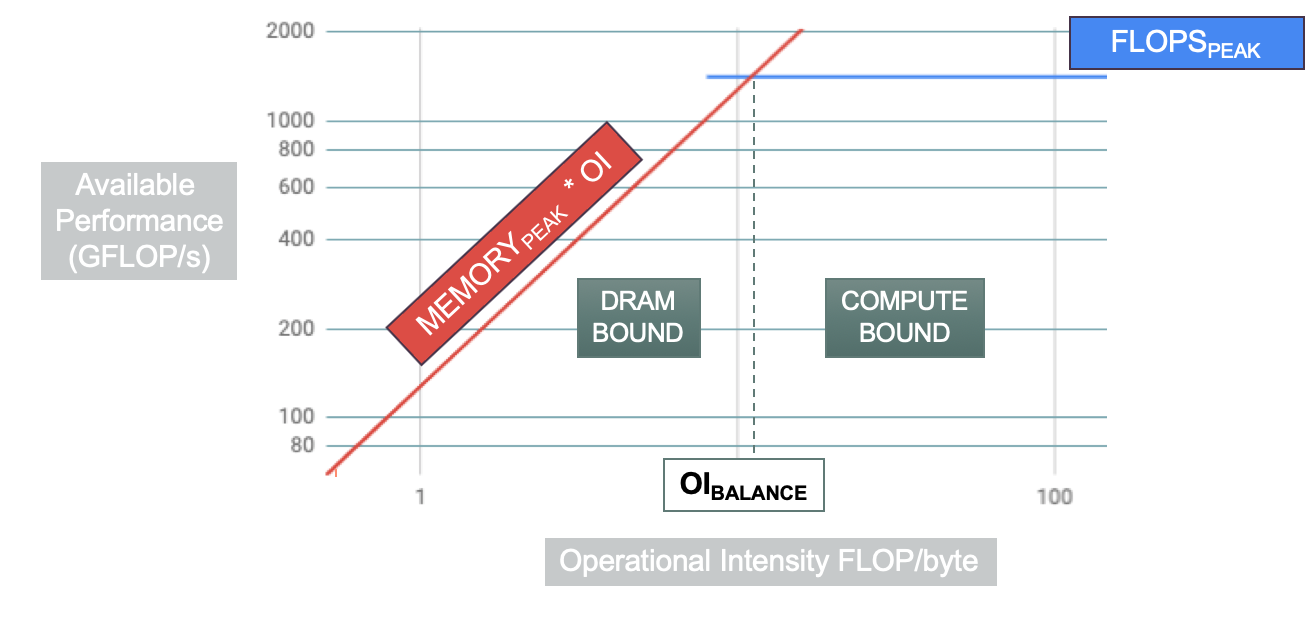
\includegraphics[width=10cm]{images/roofline.png}
    \caption{\label{fig:roofline} Représentation graphique du modèle du \textit{roofline}. En fonction de son l'intensité opérationnelle, la performance d'un code sera limitée par la bande passante ou par le processeur.}
\end{figure}


La \autoref{fig:roofline} montre une représentation du modèle du \textit{roofine}. Sur l’axe des abscisse est représentée l’intensité opérationnelle de l’algorithme (en flops/byte) qui correspond nombre d’opération flottante appliqué à chaque byte de donnée amené depuis la mémoire. Sur l’axe des ordonnées est représentée la performance de calcul mesurée en GFLOP/s.
Chaque hot spot sont placés en fonction de leur intensité opérationnelle, calculée à partir de la lecture du code, et de sa performance, mesurée lors de l’exécution.

%%%%%%%%%%%%%%%%%
\subsubsection{Preuve et construction}
%%%%%%%%%%%%%%%%%

L’objectif du modèle est de déterminer si la performance du code pour une architecture donnée est structurellement limité par la performance du processeur ($FLOPS_{peak}$ en $GFLOP/s$) ou bien par la performance du bus mémoire ($MEMORY_{peak}$ en $GB/s$). Une application réalisant la lecture de deux nombres pour y réaliser des centaines d’opérations verra ses performances limitées par la capacité de calcul $FLOPS_{peak}$ du processeur. Inversement, une application devant lire un grand jeu de données pour ne réaliser qu'une opération sur chaque valeur, verra ses performance limitées par celle du bus mémoire $MEMORY_{peak}$. On peut estimer la quantité de calculs à réaliser sur chaque donnée en calculant son Intensité Opérationnelle  ($\text{OI}$ en $flop/byte$). Pour cela il faut lire le code source pour compter manuellement le nombre d’opérations réalisées ($\text{\#FLOP}$) et le nombre de données nécessaires chargées depuis la mémoire ($\text{\#BYTE}$). On peut ainsi calculer l’Intensité Opérationnelle d’un code en faisant le ratio des deux valeurs.

\begin{equation}
\begin{aligned}
        \text{OI}_{kernel} =\ &\cfrac{\text{\#FLOP}}{\text{\#BYTE}}
\end{aligned}
\end{equation}

Le temps pour exécuter le code ($\text{TEMPS}_{theorique}$), sera le temps mis par la ressource la plus utilisée par le code. On peut estimer ce temps par la formule suivante.
\begin{equation}
\begin{aligned}
     \text{TEMPS}_{theorique} =\  &max 
     \begin{cases} 
        \quad \cfrac{\text{\#FLOP}}{\text{FLOPS}_{peak}}    \\[15pt]
        \quad \cfrac{\text{\#BYTE}}{\text{MEMORY}_{peak}}
    \end{cases}
\end{aligned}
\end{equation}




La performance théorique du code ($\text{PERF}_{theorique}$ en GFLOP/s) peut être calculée grâce aux transformations successives de l'\autoref{eq:PERFT}.
\begin{equation}
\begin{aligned}
\label{eq:PERFT}
\cfrac{\text{TEMPS}_{theorique}}{\text{\#FLOP}}  =\ &\text{max}
\begin{cases} 
    \cfrac {1}{\text{FLOPS\_{peak}}}    \\[15pt]  
    \cfrac {\cfrac{\text{\#BYTE}}{\text{MEMORY}_{peak}}}{\text{\#FLOP}} 
\end{cases}\\[20pt]
\cfrac{\text{\#FLOP}}{\text{TEMPS}_{theorique}}  =\ &\text{min}
\begin{cases} 
    \text{FLOPS}_{peak}    \\[15pt]  
    \cfrac{\text{\#FLOP}}{\text{\#BYTE}} \times \text{MEMORY}_{peak}
\end{cases}\\[20pt]
\text{PERF}_{theorique}  =\ &\text{min}
\begin{cases} 
    \text{FLOPS}_{peak}    \\[15pt]  
    \text{OI}_{kernel} \times \text{MEMORY}_{peak} 
\end{cases}
\end{aligned}
\end{equation}



Pour une architecture, il faut déterminer pour quelle intensité opérationnelle une application est limitée par la mémoire ou le processeur. Pour cela, il faut calculer l’intensité opérationnelle ($\text{OI}_{balance}$) correspondant au croisement des deux droites sur la \autoref{fig:roofline}. 

\begin{equation}
\begin{aligned}
 \text{FLOPS}_{peak} =\ &\text{OI}_{balance} \times \text{MEMORY}_{peak} \\[20pt]
 \text{OI}_{balance} =\ &\frac{\text{MEMORY}_{peak}} {\text{FLOPS}_{peak}} 
\end{aligned}
\end{equation}

Une application dont l’intensité opérationnelle est inférieure à $\text{OI}_{balance}$ verra sa performance limitée par le système mémoire. Plus rarement, si l’intensité opérationnelle d’une application est supérieure à $\text{OI}_{balance}$, la performance sera alors limitée par le processeur.

\subsubsection{Construction}
La première étape dans la construction du graphique est de tracer les deux axes limitant les performances d’un code. Ces deux droites représentes les performances crêtes de la mémoire et du processeur. Pour obtenir ces valeurs, elles peuvent être calculées à partir des spécifications du processeurs. Cependant, avec la complexification des architectures, il est difficile de les atteindre même avec des benchmarks prévus à cet effet. Il est donc préférable de les représenter par des valeurs mesurées comme indiqué dans la littérature  \cite{farjallah2014preparing}. Pour la mémoire le benchmark Stream peut être utilisé. Pour la performance du processeur, nous utilisons le générateur de benchmark présenté dans la \autoref{sec:kg}. D’autres travaux sont venus compléter les benchmarks disponibles pour caractériser l’architecture \cite{lo2014roofline}.




%%%%%%%%%%%%%%%%%
\subsubsection{Évolutions}
%%%%%%%%%%%%%%%%%


Le \textit{roofine} a reçu de nombreuse améliorations depuis sa création. En 2014, les travaux \cite{Ilic2014} constate que le modèle originale n’est pas suffisament précis à cause de la faible précision de caractérisation de l’architecture. En effet, un code pouvant profiter de la localité des données dans les caches pourrait atteindre des performances supérieur au maximum prévu par le modèle utilisant seulement le bande passante mémoire. Inversement, la performance crête est calculé pour un code utilisant tous les coeurs du processeur, avec des instructions FMA vectorisées. Cependant, par leur nature, certain code ne peuvent pas utiliser ces  caractéristiques. La performance crête étant alors impossible à atteindre. Le modèle Cache-Aware Roofline Model (CARM) \cite{Ilic2014} a ainsi été développé permettant de représenter la performance des différents niveaux de caches. Cependant, le programmeur doit comprendre si son application peut tirer partie de cette localité, ce qui peut rendre cette approche plus difficile. Le modèle à depuis été affiné avec le Locality Aware Roofline Model (LARM) \cite{Denoyelle2018} permettant de modéliser les accès en mémoire non uniforme (NUMA).
D’autres travaux essaient d’automatiser sa construction \cite{lo2014roofline} pour faciliter son usage. L’outil de profiling d’Intel a intégré les modèles CARM et LARM pour automatiser la recherche des hot spot et afficher leur performance sur un même graphique. Pour cela, il désassemble le code et calcule l’intensité opérationnelle de la boucle étudiée.


%%%%%%%%%%%%%%%%%
\subsubsection{Critiques}
%%%%%%%%%%%%%%%%%

La force de cette approche est de montrer rapidement au programmeur si son application est efficace ou non. Dans le cas échéant, il sait s’il doit travailler sur l’optimisation des flops ou de la mémoire. En modélisant les principaux kernels de son application, le programmeur saura sur lesquels ses optimisations seront le plus bénéfiques.

Bien d’ayant reçu de nombreuses améliorations, ce modèle doit être utilisé pour commencer l’analyse de performance. Mais il ne permet pas de modéliser n’y de comprendre finement la raison d’une performance.
La majorité des applications étant limitée par la bande passante mémoire, il est rare d’utiliser ce modèle pour modéliser la performances des unités de calculs. Mais il peut être intéressant de calculer l’intensité opérationnelle d’une boucle pour s’en assurer avant d’apporter des optimisations. De plus, les accélérateurs à venir essaient de réduire le trou de performance entre les processeurs et la mémoire. Cette modélisation est donc importante pour l’analyse de performance.


\bibliographystyle{StyleThese}
\bibliography{These}

%% PART 2 %%
\part{Contributions et résultats}
\chapter{Méthodologie simple pour l'analyse de performance et le portage de code}
\label{chap:methodo}
\minitoc


%%%%%%%%%%%%%%%%%%%%%%%%%%%%%%%%%%%%%%%%%%%%%%%%%%%%%%%%%%%%%%%%%%%
\section{Motivations}
%%%%%%%%%%%%%%%%%%%%%%%%%%%%%%%%%%%%%%%%%%%%%%%%%%%%%%%%%%%%%%%%%%%


\subsection{La révolution de l'hétérogénéité}

Le protocole Gen-Z, présenté dans le chapitre \ref{X}, va révolutionner le monde de l'informatique comme peu de technologies auparavant. Entre tous les bénéfices apportés par ce protocole, la faculté de rendre facile l'hétérogénéité dans les super-calculateurs est sans doute la plus importante. 

L'hétérogénéité sera à la fois entre des accélérateurs spécialisés pour différentes workload, mais aussi dans les architectures elles mêmes permettant de mixer et d'adapter chaque coprocesseur. En 2018, plus de 96\% des processeurs des super-calculateurs du Top500 ont une architecture x86 et la majorité d'entre eux (91\%) proviennent du constructeur Intel. Seulement 28\% des 500 clusters sont associés à des accélérateurs dont 92\% sont des GPU NVIDIA. Nous remarquons donc que l'architecture des super-calculateurs est très similaire et que l'utilisation d'accélérateurs adaptés n'est encore qu'à ses débuts. Aujourd'hui l'utilisation d'architectures différentes est souvent perçu négativement car elle implique d'adapter les codes, d'utiliser plusieurs langages ou d'obtenir de mauvaises performance car l'architecture n'est pas adaptée à la totalité de l'application.

Par analogie, nous comparons cette opportunité avec celle des moteurs d'avion à réaction qui ont révolutionné l'économie et le domaine de l'aviation. Si certains constructeurs et utilisateurs continuent d'utiliser la même stratégie d'ajouter des serveurs \textit{standards} comme jusqu'à aujourd'hui, ils seront dépassés par ceux ayant commencé à investir ces nouvelles technologies plusieurs années avant eux. Il est donc cruciale de s'y préparer en ayant la bonne méthodologie et les bons outils pour pouvoir en profiter. L'accès à des plate-forme exascale et à ces nouvelles architectures va aussi ouvrir de nouveaux marchés, inaccessible aujourd'hui à cause de plusieurs contraintes: le prix, la bande passante nécessaire, la sécurité ou encore la consommation électrique. 

Les gains de performance ne viendront pas seulement par l'utilisation d'accélérateurs puissants, mais de leur diversité et de la capacité des programmeurs de bien les utiliser. Pour une même application, plusieurs accélérateurs spécialisés seront souvent nécessaires. On peut en imaginer certains adaptés à la lecture et à la décompression du jeu de données. Un fois réalisé, des accélérateurs spécialisés dans le calcul demandé pourront être utilisés (ASIC, FGPA ou DSP). Enfin pour la visualisation des données, des GPU seront alors nécessaires. L'hétérogénéité est à la fois un challenge majeur des plate-formes Exascale, mais aussi une grande opportunité. 



\subsection{Développement}

Comme présente dans la section \ref{X}, l'analyse de performance peut se faire à plusieurs niveaux. En fonction de l'objectif défini, le niveau et les outils utilisés doivent être adaptés. Notre analyse porte sur la performance d'une partie du code intéressante, un hot spot. Les outils développé permettent pour le moment de mettre en avant des problèmes de performances dus au système mémoire ou au processeur. Les problèmes de performances liés au réseaux ou au système d'exploitation ne sont pas la priorité de la méthodologie, bien qu'ils puissent être décelé.

Du fait de la complexité des architectures, le travail de portage et d'optimisation peut être très difficile. Ainsi, notre démarche s'adresse aux programmeurs ayant de solides connaissances des micro-architectures. Pour améliorer la précision de l'analyse et des outils il est préférable d'avoir accès au code source. 

Contrairement à des solutions existante comme VTune \cite{vtune}, nous avons choisi de développer plusieurs outils indépendant répondant chacun à une question précise. Nous espérons qu'en réduisant la complexité de l'outillage, l'adoption des outils auprès des programmeurs sera plus grande. Les outils n'ont pas vocation d'automatiser entièrement les tâches du programmeur. La puissance de ces outils vient de leur utilisation complémentaire. 

Les outils utilisés sont disponibles en Open Source et ne sont pas exhaustifs. Certains outils utilisés ont été développé durant la thèse, d'autres répondant à nos critères n'ont pas eu à être développés de nouveau. Cette méthodologie et les outils l'accompagnant sont présentés pour partager notre philosophie d'analyse de performance, mais le travail doit être poursuivi pour ajouter de nouveaux outils. De plus, le contexte de leur utilisation est de profiter de l'hétérogénéité arrivant dans les centre de données, ils nécessiteront d'être portés sur ces architectures.



\begin{figure}
    \center
    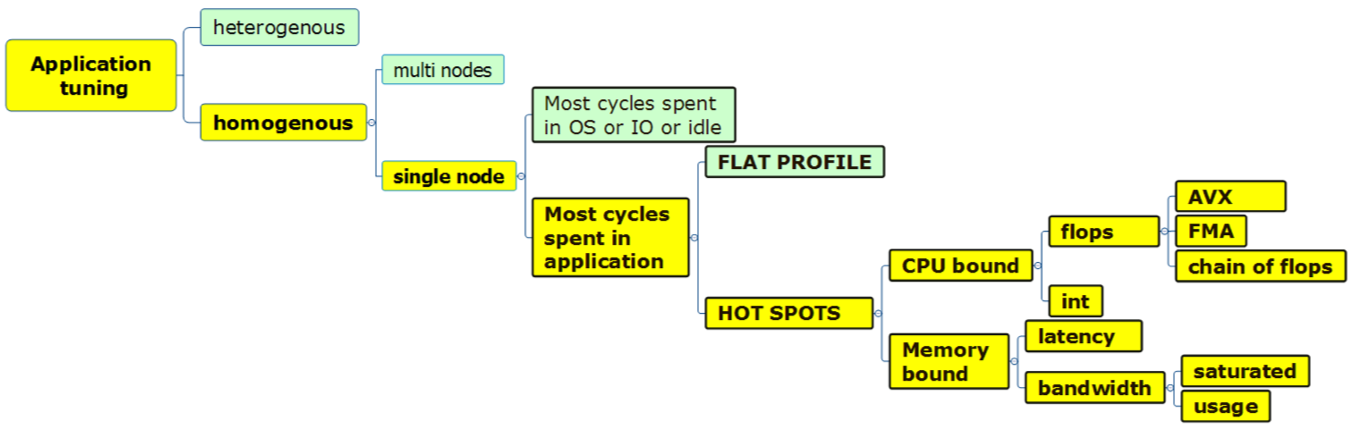
\includegraphics[width=8cm]{images/analyse.png}
    \caption{\label{pic_analyse} Délimitation de l'analyse proposée.}
\end{figure}



\subsection{Contributions}
Dans ce chapitre, nous présentons une méthodologie simple en 5 étapes permettant aux utilisateurs de modéliser les performances de leur code, de les projeter sur de nouvelles architectures et de les optimiser. Nous proposons un modèle de performance simple basé sur les caractéristiques du sous-système mémoire. L'objectif est de créer pour chaque \textit{hot spot} un modèle de ses performances dans le but de projeter ses performances sur d'autres architectures mais aussi de valider ses performances. Nous cherchons à prouver la bonne utilisation ou non du système mémoire, ressource critique pour la performance des applications sur les architectures modernes. Enfin, lorsque les performances de l'application ne sont pas celles attendues par notre modèle, nous proposons un cheminement pour comprendre, optimiser et transformer le code pour parvenir aux performances ultimes.

Pour illustrer les différentes étapes, nous appliquons la méthodologie à l'étude des performances de la fonction \textit{triadd} (voir extrait de code \ref{lst:triadd}) du benchmark Stream \cite{McCalpin1995} sur un processeur Intel\textit{ Xeon Gold 6148} possédant 20 coeurs. Les matrices utilisées mesurent chacune 19.6 GB. Cet exercice nous permet de montrer que même pour un code aussi simple et en apparence optimisée, l'approche et les outils utilisés permettent de comprendre et d'optimiser ses performances.

\begin{lstlisting}[language=c,caption=Fonction Triadd extraite du benchmark Stream \ref{McCalpin1995},label={lst:triadd}, 
  basicstyle=\footnotesize, frame=tb,
  xleftmargin=.065\textwidth, xrightmargin=.065\textwidth]
for (j=0; j < STREAM_ARRAY_SIZE; j++)
    A[j] = B[j] + scalar * C[j];
\end{lstlisting}






\iffalse 
%%%%%%%%%%%%%%%%%%%%%%%%%%%%%%%%%%%%%%%%%%%%%%%%%%%%%%%%%%%%%%%%%%%%%%%%%%%%%%%%%%%%%%%%
%%%%%%%%%%%%%%%%%%%%%%%%%%%%%%%%%%%%%%%%%%%%%%%%%%%%%%%%%%%%%%%%%%%%%%%%%%%%%%%%%%%%%%%%
%%_______ .___________.    ___      .______    _______                       __       %%
%%|   ____||           |   /   \     |   _  \  |   ____|                    /_ |      %%
%%|  |__   `---|  |----`  /  ^  \    |  |_)  | |  |__          ______        | |      %%
%%|   __|      |  |      /  /_\  \   |   ___/  |   __|        |______|       | |      %%
%%|  |____     |  |     /  _____  \  |  |      |  |____                      | |      %%
%%|_______|    |__|    /__/     \__\ | _|      |_______|                     |_|      %%
%%%%%%%%%%%%%%%%%%%%%%%%%%%%%%%%%%%%%%%%%%%%%%%%%%%%%%%%%%%%%%%%%%%%%%%%%%%%%%%%%%%%%%%%
%%%%%%%%%%%%%%%%%%%%%%%%%%%%%%%%%%%%%%%%%%%%%%%%%%%%%%%%%%%%%%%%%%%%%%%%%%%%%%%%%%%%%%%%
\fi


%%%%%%%%%%%%%%%%%%%%%%%%%%%%%%%%%%%%%%%%%%%%%%%%%%%%%%%%%%%%%%%%%%%
\section{Étape 1: Veille technologique}
%%%%%%%%%%%%%%%%%%%%%%%%%%%%%%%%%%%%%%%%%%%%%%%%%%%%%%%%%%%%%%%%%%%

%%%%%%%%%%%%%%%%%
\subsection{Motivation et objectifs}
%%%%%%%%%%%%%%%%%

Grâce à Gen-Z, de nouvelles technologies utilisable par les super-calculateurs vont apparaître régulièrement. Comme expliqué précédemment, il est crucial pour les utilisateurs de porter leur code et d'investir du temps et de l'argent dans les bonnes plate-formes. Aujourd'hui ce choix se limité à quelques architectures, principalement les CPU (Intel, AMD, IBM) et les accélérateurs (NVIDIA, AMD, Xeon Phi). Demain, prendre la bonne entre toutes les nouvelles technologies sera beaucoup plus difficile.

Même si elle n'est pas une étape de la méthodologie en soit, le premier travail de développeur est d'être en constante recherche des dernières innovations technologiques. Cela peut être de nouveau processeurs, de nouvelles mémoire ou bien de nouveaux algorithmes ou optimisations. Il est très important de se tenir à l'état de l'art ou même en avance pour anticiper les nouveautés. 

Le but principal de cette étape est de répertorier toutes les plate-formes et technologies potentiellement intéressantes pour le calcul haute performance. Certaines caractéristiques clés sont calculées à partir des spécificités techniques des architectures.


%%%%%%%%%%%%%%%%%
\subsection{Processeurs et accélérateurs}
%%%%%%%%%%%%%%%%%

Dans notre vision, la majorité des lignes de codes continueront d'être exécutées sur des architectures semblables à celles d'aujourd'hui (x86 et PowerPC). Seulement les kernels de calculs seront déportés sur les accélérateurs adéquats. Il est donc nécessaire de continuer à s'y interesser et à les caractériser. Les processeurs présent dans les architectures de demain pourraient alors être bien différent de ce d'aujourd'hui car si les kernels des applications n'y sont plus exécutés, les caractéristiques recherchés seront différentes. 

Les accélérateurs actuels continueront d'avoir leur rôle à jouer. Les GPU se sont montrés extrêmement efficace pour les algorithmes d'apprentissage par machine et d'intelligence artificielle.



%%%%%%%%%%%%%%%%%
\subsection{Mémoires}
%%%%%%%%%%%%%%%%%

Grâce à Gen-Z, la totalité de l'architecture sera \textit{composable}, pas seulement au niveau des processeurs mais aussi au niveau des mémoires. Grâce à sa sémantique d'accès \textit{load/store}, Gen-Z va permettre au processeur d'accéder à toute la mémoire visible dans le super-calculateur. En fonction des jeux de données, la quantité de mémoire doit être calculée pour de pas en manquer et risquer d'effondrer les performances, ou de surestimer le besoin et perdre en rendement économique. 



%%%%%%%%%%%%%%%%%
\subsection{Caractéristiques clefs}
%%%%%%%%%%%%%%%%%

Pour la suite de l'analyse, il est nécessaire de récupérer des caractéristiques clefs pour chaque architectures. Cette phase étant indépendante de l'application, il ne faut pas négliger certaines architectures qui pourraient s'avérer intéressante ensuite. La majorité des applications aient besoin d'un bus mémoire très performant. Seulement, certaines partie du code, séquentielles ou utilisant seulement les unités arithmétiques et logiques, auront d'autres besoins qui pourra être interessant de porter sur des architectures différentes.

Nous avons isolé X caractéristiques qu'il est nécessaire d'avoir pour la suite de l'analyse:
\begin{itemize}
    \item La bande passante économique dont qui mesure le nombre de gigabyte de données transférable par seconde pour le prix de la plate-forme ($GB/seconde/dollar$). Deux facteurs très important dans le choix de la plate-forme entre ici en jeu: la bande passante disponible, très importante pour la majorité des codes, ainsi que l'économie qui est souvent le facteur de décision ultime. On cherchera les plate-forme avec la plus grande bande passante économique.
    \item L'équilibre arithmétique de la plate-forme est mesurée nombre d'opération réalisable pour chaque gigabyte de données transféré  depuis la mémoire en une seconde mesuré en  $flops/GB/s)$. Cette valeur permet d'estimer l'équilibre entre le calcul et le débit mémoire d'une plate-forme. Une grande valeur signifiera que la plate-forme est plutôt destinée à des codes intensifs en calcul. A l'inverse, une valeur faible signifiera que la plate-forme est adapté à des codes nécessitant beaucoup d'accès mémoire. Pour la majorité des applications on cherchera à obtenir une valeur petite.
    \item L'efficience énergétique mesure le rapport d'opérations flottante par watt d'énergie consommée ($flops/watt$). Comme exposé dans la partie \ref{X}, la consommation électrique du super-calculateur est une contrainte majeur pour le projet Exascale. Il est donc important de privilégier des architectures avec les meilleurs rendements énergétiques. On cherche ici à obtenir la plus grande valeur possible.
\end{itemize}




%%%%%%%%%%%%%%%%%
\subsection{Calculs des caractéristiques}
%%%%%%%%%%%%%%%%%

Le calculs des caractéristiques par les données techniques des architectures a l'avantage de permettre d'évaluer rapidement leur potentiel sans y avoir accès. Cette partie présente comment calculer certaines caractéristiques comme la bande passante ou la puissance crête d'un processeur.

%%%%%%%%%%%%%%%%%
\subsubsection{La bande passante}
Le calcul de la bande passante mémoire, nécessite de connaître la fréquence de la mémoire mesurée en $MHz$. La fréquence de la mémoire RAM correspond au nombre de cycle d'horloge par seconde. Il existe différentes technologies mémoire permettant d'écrire entre une, deux ou quatre fois par cycle sur chaque ligne du bus. On parle alors de mémoire Single Data Rate (SDR), Double Data Rate (DDR) et Quad Data Rate (DQR). La fréquence seule ne permet donc pas d'indiquer combien de transferts peuvent être réalisés par seconde, il faut aussi connaître le débit de données. Pour éviter les confusions, on parle aussi de Mega Transferts par seconde ($MT/s$) que l'on notre $MTS$. Ces deux unités sont souvent mélangés, par les constructeurs eux même, peut être à des fins marketing. Par exemple la DDR4-2666, signifie que la RAM a une fréquence de 1333 MHz. Il faut ensuite connaître le nombre de ligne reliant la mémoire au processeur ou au GPU que l'on note $bus\_width$ mesuré en byte. Les architectures x86 récentes utilisent des bus de 64 bits. Pour augmenter la bande passante mémoire disponible, les architectures utilisent plusieurs canaux mémoire noté $nb\_channels$.
La bande passante maximum théorique, $MEMORY_{peak}$, peut alors être calculée avec la formule suivante:

\begin{equation}
\label{eq:bw}
    MEMORY_{peak} = MTS \times bus\_width \times nb\_channels
\end{equation}


%%%%%%%%%%%%%%%%%
\subsubsection{La puissance de calculs}
La deuxième valeur qui nous intéresse dans notre analyse est la performance crête de calcul mesurée en $GFlops$. Pour la calculer, nous adaptons la notation proposée dans \cite{dolbeau2015theoretical}.
La première information nécessaire est le nombre maximale de \textit{flop} exécutable par cycle, notée $FLOP_{cycle}$ mesuré en $\frac{flop}{cycle}$. 
Les processeurs sont capables de réaliser des opérations sur plusieurs données à la fois. La taille de ces instructions (SIMD) et leur disponibilité dépend de l'architecture. Elle est mesurée en $\frac{flop}{operation}$.
Pour atteindre la performance crête, il faut utiliser les instructions permettant de faire le maximum d'opération en une exécution. Sur les processeurs modernes ce sont les instructions Fused Multiply Add (FMA) qui sont capables d'exécuter une multiplication et une addition en un cycle mesuré en $\frac{operations}{instruction}$. Enfin, les processeurs superscalaire sont capables d'exécuter plusieurs instructions en un seul cycle, mesurée en $\frac{instructions}{cycle}$. $FLOP_{cycle}$ peut ainsi être calculé grâce à la formule suivante:

\begin{equation}
\label{eq:floc}
    FLOP_{cycle} = \frac{flop}{operation} \times \frac{operations}{instruction} \times \frac{instructions}{cycle}
\end{equation}

Une fois la performance maximale de la micro-architecture calculée, il faut calculer la performance maximale atteignable par le processeur, notée $FLOP_{seconde\_peak}$ mesurée en $\frac{flop}{seconde} $. Pour cela, il faut connaître la fréquence atteignable par le processeurs lorsque sont exécutés les instructions SIMD utilisées pour calculer $FLOP_{cycle}$. En effet, pour éviter des problèmes de surchauffe, le processeur doit abaisser sa fréquence lorsqu'il utilise de telles instructions. Cette fréquence est notée $\frac{cycle}{seconde}$. Enfin, il faut avoir le nombre de coeurs disponibles sur le processeurs.
\begin{equation}
\label{eq:flops}
    FLOP_{seconde\_peak} = FLOP_{cycle} \times \frac{cycle}{seconde} \times nombre\ de\ coeurs
\end{equation}





%%%%%%%%%%%%%%%%%
\subsection{Application au processeur Intel Xeon 6148}
%%%%%%%%%%%%%%%%%

Pour illustrer la présentation de la méthodologie, nous utilisons l'exemple d'un processeur Intel Xeon Skylake 6148 possédant 20 coeurs à une fréquence de base de 2.4 GHz. Une configuration à deux processeurs est présenté sur la \autoref{fig:skylake_gold}. \textbf{Mémoire: } le processeur étudié possède 6 canaux mémoire le connectant à 6 barrettes mémoire cadencé à 2666 MT/s. \textbf{ALU:} les processeurs de la gamme Xeon Gold 6 possèdent tous deux unités AVX-512 capables d'exécuter chacune 2 instructions vectorielles de 512 bits (AVX-512), dont les Fused Multiple Add (FMA). \textbf{Fréquence:} pour une même architecture, dans notre exemple Skylake, chaque modèle de processeur a ses propres plages de fréquences utilisables qui peuvent être consultées en ligne \cite{Wikichipa}. La fréquence utilisable dépend essentiellement de la consommation électrique du processeur et de sa température (dépendant de la qualité du système de refroidissement). Ainsi, les fréquences soutenables par le processeurs dépendent du nombre de coeurs utilisés, de la taille des instructions  exécutées (normal, AVX-2 ou AVX-512) et de la disponibilité du Turbo. Pour l'exécution d'instruction SISD (Single Instruction Single Data) avec le turbo actif sur les 20 coeurs, la fréquence maximale atteignable est de 3.1 GHz.  Le benchmark étudié a la possibilité d'utiliser des instructions vectorielles, le processeur Skylake 6148 peut utiliser des fréquence allant de 1.6 GHz à 2.2GHz \cite{Wikichipa}. 

\begin{figure}
    \center
    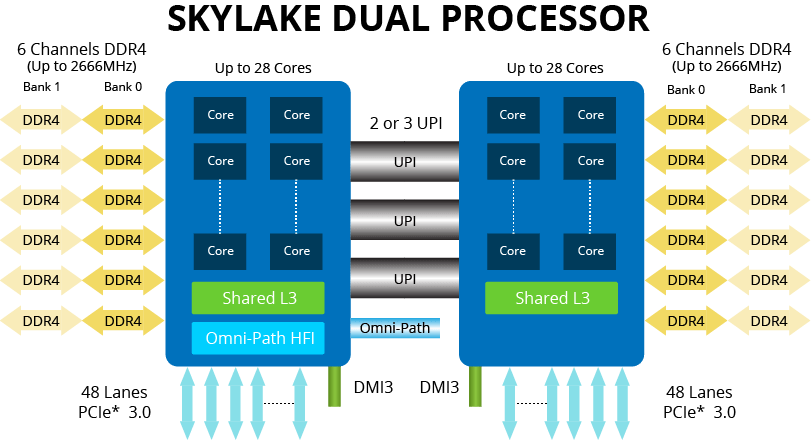
\includegraphics[width=10cm]{images/skylake_gold.png}
    \caption{\label{skylake_gold} Architecture d'une plate-forme avec deux processeurs Xeon Skylake (source \cite{Aspsys})}
\end{figure}



%%%%%%%%%%%%%%%%%
\subsubsection{Performances mémoire théoriques}
Le processeur Xeon Skylake 6148 possède 6 canaux mémoire pour accéder, dans notre expérimentation, à une mémoire DDR4-2666. En appliquant l'\autoref{eq:bw} nous obtenons une bande passante maximale de : $2666 \times 8 \times 6 = 128\ GB/s$. A cause de la loi de Little \cite{little2008little}, le processeur doit être capable de générer parallèlement suffisamment de chargement (\textit{outstanding load}) pour atteindre cette performance.


%%%%%%%%%%%%%%%%%
\subsubsection{Performances de calculs théoriques}
Le processeur étudié est un processeur superscalaire capable d'éxécuter jusqu'à 4 instructions par cycle dont deux opérations flottantes. Ces opération pouvant être des instruction FMA vectorielles de 512 bits. Il est donc possible de calculer sur chaque ALU, une multiplication et une addtion par cycle sur 8 éléments simultanément. On peut ainsi calculer la performances crête de ce processeur en appliquant l'\autoref{eq:flops}. Suivant la fréquence utilisable par le processeur (dépendant de la température) la performance crête théorique, $FLOPS_{peak}$ est comprise entre $8 \times 2 \times 2 \times 1.6 \times 20 = 1024\ GFLOP/s$ et  $8 \times 2 \times 2 \times 2.2 \times 20 = 1408\ GFLOP/s$. 

Cependant, pour comparer la performance de l'application avec ce résultat, il faut que la nature du code puisse utiliser des instructions FMA vectorisées. Il peut être intéressant de disposer d'une fourchette de performance lorsque la totalité du parallélisme est utilisé ou non. Quand le processeur n'utilisent pas d'instruction AVX-512, le processeur est capable d'atteindre 3.1 GHz lorsque les 20 coeurs sont actifs. En reprenant l'\autoref{eq:flops}, la performance optimale d'une telle application serait: $FLOPS_{SISD} = 1 \times 1 \times 2 \times 3.1 \times 20 = 124 \ GFLOP/s$.

%%%%%%%%%%%%%%%%%
\subsubsection{Équilibre arithmétique}
L'équilibre arithmétique du processeur permet d'évaluer s'il est approprié pour un code nécessitant une grande bande passante ou plutôt de bonnes performances de calculs. En réutilisant les deux caractéristiques précédemment calculées, on peut calculer $\text{EQUILIBRE}_{non\_avx}$ et $\text{EQUILIBRE}_{avx\_512}$ qui bornent la performances inférieure et supérieure de ce processeur. On obtient ainsi $\text{EQUILIBRE}_{non\_avx} = \frac{124}{128} = 0.97\ flop/byte$ et $EQUILIBRE_{avx\_512} = \frac{1408}{128} = 11\ \text{flopbyte}$. 
 

%%%%%%%%%%%%%%%%%
\subsubsection{L'efficacité énergétique}

La valeur  $EQUILIBRE_{avx\_512}$ est la plus pertinente des deux pour réaliser le choix de l'architecture. Les composants permettant de faire du calcul vectoriel sont compris dans le prix d'achat, qu'ils soient utilisés ou non. Si l'application portée est loin du ratio de 11 opérations flottantes pour 1 byte de données transféré, il faudra se tourner vers d'autres architecture, plus efficace. La notion d'efficacité se retrouve dans le ratio $flops/watt$.
\\
\textbf{todo}






















\iffalse 
%%%%%%%%%%%%%%%%%%%%%%%%%%%%%%%%%%%%%%%%%%%%%%%%%%%%%%%%%%%%%%%%%%%%%%%%%%%%%%%%%%%%%%%%
%%%%%%%%%%%%%%%%%%%%%%%%%%%%%%%%%%%%%%%%%%%%%%%%%%%%%%%%%%%%%%%%%%%%%%%%%%%%%%%%%%%%%%%%
%%_______ .___________.    ___      .______    _______                      ___       %%
%%|   ____||           |   /   \     |   _  \  |   ____|                   |__ \      %%
%%|  |__   `---|  |----`  /  ^  \    |  |_)  | |  |__          ______         ) |     %%
%%|   __|      |  |      /  /_\  \   |   ___/  |   __|        |______|       / /      %%
%%|  |____     |  |     /  _____  \  |  |      |  |____                     / /_      %%
%%|_______|    |__|    /__/     \__\ | _|      |_______|                   |____|     %%
%%%%%%%%%%%%%%%%%%%%%%%%%%%%%%%%%%%%%%%%%%%%%%%%%%%%%%%%%%%%%%%%%%%%%%%%%%%%%%%%%%%%%%%%
%%%%%%%%%%%%%%%%%%%%%%%%%%%%%%%%%%%%%%%%%%%%%%%%%%%%%%%%%%%%%%%%%%%%%%%%%%%%%%%%%%%%%%%%
\fi


%%%%%%%%%%%%%%%%%%%%%%%%%%%%%%%%%%%%%%%%%%%%%%%%%%%%%%%%%%%%%%%%%%%
\section{Étape 2: Caractérisation des plate-formes}
%%%%%%%%%%%%%%%%%%%%%%%%%%%%%%%%%%%%%%%%%%%%%%%%%%%%%%%%%%%%%%%%%%%

%%%%%%%%%%%%%%%%%
\subsection{Motivations et objectifs}
%%%%%%%%%%%%%%%%%

Pour pouvoir estimer la bonne ou mauvaise performance d'un code sur une plate-forme il est nécessaire de connaître la performance crête de cette dernière. Cette approche est utilisée par le modèle du \textit{roof line}. L'approche présentée dans cette thèse nécessite s'intéresse aux mêmes caractéristiques qui sont: la bande passante mémoire ($GB/s$) et la capacité calculatrice ($FLOP/s$). Il y a deux façons d'obtenir ces performances crêtes. La première méthode est de la calculer à partir des caractéristiques techniques de la plate-forme. Cette méthode à été utilisé lors de l'étape 1 permet de catégoriser les plate-formes qui pourront être envisagées pour porter l'application. La deuxième méthode est de la mesurer lors de l'exécution de l'application ou de benchmark. Pour la réalisation de cette étape, il faut avoir accès aux matériels pour pouvoir y réaliser les mesures. Des simulateurs peuvent aussi être utilisés bien que cette étape servent à mesurer les performances réelles de l'architecture.





%%%%%%%%%%%%%%%%%
\subsection{Mesure effective}
%%%%%%%%%%%%%%%%%
Une application industrielle peut être difficile à porter sur une nouvelle architecture dans le simple but de la caractériser. Il est préférable d'utiliser des benchmarks, plus court et plus facilement portable. Ces codes, souvent simple, permettent de caractériser une ou plusieurs parties d'une architecture. Cette valeur valeur est souvent inférieur à la performance théorique du fait de la complexité des architectures ou de la qualité du code généré. Par exemple pour mesurer la bande passante mémoire maximale atteignable on peut utiliser le benchmark \textit{Stream} \cite{McCalpin1995}, les latences des différents niveaux de caches \textit{lmbench} \cite{Staelin2002}. Pour mesurer le nombre maximum d'opération sur un nombre flottant exécutables par seconde, on peut utiliser le benchmark Linpack. 
L'avantage de cette approche est sa facilité. Il suffit de compiler le benchmark voulu et de l'exécuter pour obtenir les résultats. Si le code est optimale, cette méthode permet de mesurer la performance maximale réelle atteignable par l'architecture. Ainsi pourra comparer les performances de l'application avec les performances maximales atteignables par la plate-forme. 

L'inconvénient est que la mesure est dépendant de la qualité de code et du compilateur. Il peut arriver qu'en voulant mesurer spécifiquement un composant, les performances soient dégradées par une autre partie du sous système, empêchant ainsi la caractérisation exacte dont nous avons besoin. Par exemple, si l'on cherche à mesurer la bande passante maximale atteignable par un seul coeur avec un code simple lisant un tableau de données. Sur un processeur récent tel qu'un Xeon Skylake, on s'attendrait à obtenir une valeur proche du maximum théorique de 128 GB/s, calculé dans la partie précédente. Cependant, à cause de la Loi de Little \cite{little2008little} et de la taille de la queue de chargement (\textit{outstanding load queue}), il faut plus de dix coeurs actifs pour saturer la bande passante \cite{JohnMcCalpin2010}. Il faut donc une certaine expérience des outils et des micro-architectures pour apprécier les résultats mesurées. Il peut ainsi être nécessaire d'avoir plusieurs codes de benchmark à exécuter pour valider de différentes façon la micro-architecture. Nous avons développé un benchmark mémoire (section \ref{aaa}) et un benchmark de calcul (section \ref{bbbb}) pour générer différentes versions et évaluer une plate-forme le plus précisément possible.





%%%%%%%%%%%%%%%%%
\subsection{Application au processeur Intel Xeon 6148}
%%%%%%%%%%%%%%%%%
Nous mesurons les performances crête du bus mémoire, $\text{MEMORY}_{max}$ en GB/s, et du processeur $FLOP_{seconde\_max}$ en GFLOP/s, en utilisant deux contributions de la thèse: le benchmark mémoire \textit{dml\_mem} et le générateur de kernel, \textit{kernel\_generator}.


%%%%%%%%%%%%%%%%%
\subsubsection{Performances mémoires}


\textbf{Bande passante mesurée}
Nous utilisons le benchmark mémoire présenté dans \autoref{sec:dml}. A cause de la loi de Little \cite{little2008little}, nous utilisons la version MPI du benchmark sur les 20 coeurs pour s'assurer de saturer le bus mémoire grâce à la commande présentée dans \autoref{lst:dmlmem_xeon}. Nous obtenons une bande passante mémoire $\text{MEMORY}_{max}$ de 105 GB/s que nous avons vérifié avec l'outil \textit{YAMB}.\\

\begin{lstlisting}[caption=Commande utilisée pour obtenir la bande passante maximale avec le benchmark \textit{DML\_MEM}, label={lst:dmlmem_xeon},
  basicstyle=\footnotesize, frame=tb,
  xleftmargin=.065\textwidth, xrightmargin=.065\textwidth]
mpirun -np 20 numactl dml_mem  --steplog 0 --unroll 8 
       --type read --stride 64 --matrixsize 5000
\end{lstlisting}


%%%%%%%%%%%%%%%%%
\subsubsection{Performance de calculs}


\textbf{Performance de calculs mesurée}: nous utilisons le générateur de benchmark \textit{Kernel\_Generator} (voir \autoref{seq:kg}) pour évaluer le nombre maximum d'opérations FMA AVX-512 réalisable sur un nombre flottant à double précision. Pour cela nous avons utilisé la commande présentée dans l'\autoref{code:kg_512}. Nous générons un kernel de 14 instructions FMA pour réduire le coût de gestion de la boucle (incrémentation et comparaison) et masquer la latence des instructions.\\

\begin{lstlisting}[caption=Commande utilisée pour obtenir la performance crête du processeur (GFLOP/s) avec le générateur de benchmark \textit{Kernel\_Generator}., label={code:kg_512},
  basicstyle=\footnotesize, frame=tb,
  xleftmargin=.065\textwidth, xrightmargin=.065\textwidth]
./kg -W 512 -O ffffffffffffff -P double -S 100 -L 120000000
\end{lstlisting}


Le benchmark généré ne possède pas de version multi-coeurs, nous lançons donc indépendamment 20 exécutions du binaire que l'on accroche à un coeur différent grâce à un paramètre du benchmark. Pour cette expérience nous avons commencé par désactiver le turbo du processeur, et limité sa fréquence à 1.6GHz. La performance mesurée est de 998.57 GFLOP/s. Ensuite nous avons activé le turbo, et laissé le processeur choisir lui même sa fréquence. L'\autoref{code:kg_512_output} montre les résultats donnés par le benchmark pour l'exécution sur un des 20 coeurs. Le benchmark mesure sa fréquence effective et trouve bien la valeur de 2.2 GHz renseigné par Intel dans sa documentation. La performance crête d'un coeur est de 69.2 GFLOP/s, approchant le maximum théorique de 70 GFlop/s.


\begin{lstlisting}[caption=Résultat de l'exécution du benchmark sur un coeur avec le turbo activé, label={code:kg_512_output},
  basicstyle=\footnotesize, frame=tb,
  xleftmargin=.005\textwidth, xrightmargin=.005\textwidth]
------------------  INSTRUCTIONS SUMMARY ------------------------------
_label_|   NB INSTRUCTIONS      Time    FREQUENCY    inst/sec       IPC
_value_|      168000000000      38.8          2.2     4.33e+9      2.01
----------------------  FLOP SUMMARY  ---------------------------------
 PRECISION     FLOP/cycle         FLOP/second
    Single              0                   0
    Double           32.0            6.92e+10
-----------------------------------------------------------------------
\end{lstlisting}

Pour vérifier que les 20 coeurs effectuaient bien le même travail, un outil de profilage développé en interne, appelé \textit{mygflops.sh}, a été utilisé. Il permet de compter les instructions flottantes simple et double précision exécutées sur un processeur. Le résultat est présenté dans l'\autoref{code:mygflops_512_output}. La performance crête mesurée du processeur est de 1372.78 GFlop/s, proche du maximum théorique calculé précédemment de 1408 GFLOP/s.

\begin{lstlisting}[caption=Résultat de l'outil \textit{myflops.sh} utilisé pour compter les instructions flottante exécutées sur un processeur., label={code:mygflops_512_output},
  basicstyle=\footnotesize, frame=tb,
  xleftmargin=.005\textwidth, xrightmargin=.005\textwidth]
Single-precision SSE/AVX :       0.00 GFlop/s  --   0.0% of Flops
Double-precision SSE/AVX :     (*\bfseries 1372.78 GFlop/s*)  -- 100.0% of Flops
   0.0% scalar  64-bit SSE/AVX instructions (  0.0% of fp instructions)
   0.0% packed 128-bit SSE/AVX instructions (  0.0% of fp instructions)
   0.0% packed 256-bit AVX instructions     (  0.0% of fp instructions)
 100.0% packed 512-bit AVX instructions     (100.0% of fp instructions)
\end{lstlisting}












 
 
 
 






%%%%%%%%%%%%%%%%%%%%%%%%%%%%%%%%%%%%%%%%%%%%%%%%%%%%%%%%%%%%%%%%%%%%%%%%%%%%%%%%%%%%%%%%
%%%%%%%%%%%%%%%%%%%%%%%%%%%%%%%%%%%%%%%%%%%%%%%%%%%%%%%%%%%%%%%%%%%%%%%%%%%%%%%%%%%%%%%%
%%_______ .___________.    ___      .______    _______                      ___       %%
%%|   ____||           |   /   \     |   _  \  |   ____|                   |___ \     %%
%%|  |__   `---|  |----`  /  ^  \    |  |_)  | |  |__          ______        __) |    %%
%%|   __|      |  |      /  /_\  \   |   ___/  |   __|        |______|      |__ <     %%
%%|  |____     |  |     /  _____  \  |  |      |  |____                     ___) |    %%
%%|_______|    |__|    /__/     \__\ | _|      |_______|                   |____/     %%
%%%%%%%%%%%%%%%%%%%%%%%%%%%%%%%%%%%%%%%%%%%%%%%%%%%%%%%%%%%%%%%%%%%%%%%%%%%%%%%%%%%%%%%%
%%%%%%%%%%%%%%%%%%%%%%%%%%%%%%%%%%%%%%%%%%%%%%%%%%%%%%%%%%%%%%%%%%%%%%%%%%%%%%%%%%%%%%%%


%%%%%%%%%%%%%%%%%%%%%%%%%%%%%%%%%%%%%%%%%%%%%%%%%%%%%%%%%%%%%%%%%%%
\section{Étape 3: Extraction de kernels et modélisation de leur performance}
%%%%%%%%%%%%%%%%%%%%%%%%%%%%%%%%%%%%%%%%%%%%%%%%%%%%%%%%%%%%%%%%%%%


%%%%%%%%%%%%%%%%%
\subsection{Motivations et objectifs}
%%%%%%%%%%%%%%%%%



Les applications que nous ciblons dans notre analyse sont des codes dont la majorité du temps d'exécution se déroule seulement dans quelques pourcentages des lignes de codes. Nous appelons ces zones des points chauds, \textit{hot spots} ou encore \textit{kernels}. Une application possédant des hot spots est un gage d'un potentiel d'amélioration des performances. Les applications réelles utilisées en production dépassent souvent les dizaines de milliers de lignes de codes. Porter et optimiser la totalité d'une application serait complexe et contre-productif. De plus, le portage et l'optimisation des codes est une tâche difficile, même aujourd'hui alors que le nombre d'accélérateurs différents disponibles est réduit. Ensuite, pour optimiser la phase de transformation du code, nous modélisons la performances de ces kernels pour éliminer les plate-formes inadaptées. Ce nombre peut encore être réduite grâce au caractéristiques récupérées lors de l'étape 2.  


L'objectif de cette étape est d'identifier ces zones du code clés et de modéliser leur performances en fonction des performances de la bande passante mémoire (GB/s) ou du processeur (FLOP/s) en calculant leur intensité opérationnelle $\text{OI}_{kernel}$. La majorité des codes étant limité par la performance de la mémoire, la thèse présente un modèle de performance basé sur ses performances. 


%%%%%%%%%%%%%%%%%
\subsection{Identification des kernels}
%%%%%%%%%%%%%%%%%

Si une application passe 99\% de ses cycles dans l'exécution d'une fonction, une amélioration d'un facteur 10 de celle-ci entraînera une amélioration du même facteur de l'application. L'identification des ces fonctions est donc primordiale. 

De nombreux travaux sont réalisés pour identifier et extraire les \textit{hot spots} d'une application \cite{castro2015cere, brunst2013custom}. L'outil de profilage \textit{perf} \cite{de2010new} permet d'extraire un sommaire de l'exécution d'une application en représentant son arbre d'appel (voir \autoref{perf_example}). 



\begin{lstlisting}[caption=Exemple d'utilisation de l'out perf avec la commande \textit{perf record  -g  -F 97}. Le rapport d'exécution est obtenu avec la commande \textit{perf report --stdio}, float,floatplacement=H, label={perf_example}]
# Samples: 116K of event 'cycles:ppp'
# Event count (approx.): 2744862582690
#
# Children      Self  Command          Shared Object       Symbol                                                                       
# ........  ........  ...............  .................. .......
    99.52%     0.00%  Stream.SKL.128   [unknown]           [k] 0000000000000000
            |          
             --99.52%--0
                       |          
                        --99.16%--0xadf96
                                  |
                                  |--25.35%--tuned_STREAM_Add   
                                  |--25.34%--tuned_STREAM_Triad
                                  |--20.36%--tuned_STREAM_Copy
                                  |--17.27%--tuned_STREAM_Scale
                                   --10.74%--main

\end{lstlisting}



%%%%%%%%%%%%%%%%%
\subsection{Modélisation de l'équilibre des kernels}
%%%%%%%%%%%%%%%%%

Chaque kernel peut être porté sur un accélérateur différent, et leur analyse doit se faire indépendamment les uns des autres. L'objectif de la modélisation est de comprendre les performances de l'application: si elles limitées par les performances du sous système mémoire ou par la capacité de calcul du processeur. La modélisation des performances permet de réduire le nombre de plate-forme envisagées pour le portage de l'application. Cette étape permet d'éviter d'investir du temps et de l'argent dans des solutions inefficace pour l'application étudiée. La modélisation du kernel nécessite de lire son code pour compter les différents accès mémoire et les opérations réalisées.

La majorité des codes HPC exécutées sur des architectures modernes voient leurs performances limitées par celle de la bande passante mémoire. S'il est très rare de voir un code limité par la puissance de calcul, il peut être nécessaire de faire cette vérification. 

Pour cela, le \textit{Roof Line Model}, permet de réaliser cette représentation des performances. Il est présenté dans la section \ref{sec:roofline}. 

Il est nécessaire de calculer l'intensité opérationnelle, $\text{OI}_{kernel}$, mesurée en $flop/byte$. Elle représente le nombre d'opération réalisable par le processeur pour chaque donnée transférée depuis la mémoire. Ce calcul se fait à partir de la lecture de code source, motivant le désire des programmeurs d'identifier individuellement les kernels de calculs. 


%%%%%%%%%%%%%%%%%
\subsection{Simple Memory Model: Modélisation de la performance mémoire} \label{sec:smm}
%%%%%%%%%%%%%%%%%

La majorité des codes étant limité par la performance du système mémoire, nous avons développé un modèle de performance simple, permettant de modéliser et valider les performances d'un code facilement. Pour réaliser cette modélisation le développeur doit avoir accès au code source de l'application à porter. Pour un hot spot donné, il faut compter le nombre d'accès mémoire en distinguant les accès en lecture et ceux en écriture. Il est important de distinguer les accès en lecture et en écriture car nous utiliserons leur ratio pour valider le bon comportement de la micro-architecture avec l'outil YAMB. En effet, nous montrons dans notre expérience que la saturation du bus mémoire n'est pas un indicateur suffisant pour conclure de l'efficacité ou non d'un code.

Cette modélisation est faisable seulement si les kernels du code ont été identifiés, l'appliquer sur la totalité de l'application serait trop long. Si la taille des jeux de données $\text{DATA}_{size}$ est connue, il est alors possible de calculer la quantité de donnée minimale qui doit être transférée sur le bus mémoire. Grâce à l'étape 2, nous connaissons les performances maximales théorique $\text{MEMORY}_{peak}$ et réelle $\text{MEMORY}_{max}$ de la micro-architecture. Il est donc possible de calculer la durée optimale pour exécuter fonction étudiée, $\text{TEMPS}_{optimal}$, mesurée en seconde. Le modèle assume que le code utilise un algorithme parfait (utilisation de la localité des données), que sa compilation du code à été réalisée avec un compilateur parfait et qu'il est exécuté sur une plate-forme parfaite. L'objectif n'est pas d'atteindre exactement cette performance, mais de s'en approcher le plus possible. Généralement, lorsque qu'un défaut apparaît à un des niveaux énuméré précédemment, la performance s'éloigne radicalement de la performance optimale.

\begin{equation}
    \text{TEMPS}_{optimal}\ = \frac{\text{DATA}_{size}}{\text{MEMORY}_{max}}
\end{equation}





%%%%%%%%%%%%%%%%%
\subsection{Application des modèles roofline et SMM au benchmark Stream}
%%%%%%%%%%%%%%%%%

L'\autoref{perf_example} montre le profil de l'exécution du benchmark \textit{Stream}. Il comporte quatre fonctions utilisées pour stresser la mémoire par différent type d'accès. Nous choisissons arbitrairement de consacrer notre analyse sur un des quatre \textit{hot spot} de Stream: la fonction \textit{triad} dont le code peut être vu dans l'\autoref{code:triad}. Cette fonction est intéressante car ce motif d'accès est très courant dans les applications HPC (algorithmes RTM).

\subsubsection{Modèle du roofline}
%%%%%%%%%%%%%%%%%
La première étape est de modéliser l'équilibre entre processeur et mémoire des besoins de l'application. 

\begin{lstlisting}[language=c,caption= La fonction triad du benchmark Stream utilise trois matrices: deux en lecture et une en écriture,label={code:triad}, 
  basicstyle=\footnotesize, frame=tb,
  xleftmargin=.065\textwidth, xrightmargin=.065\textwidth]
for (j=0; j < STREAM_ARRAY_SIZE; j++)
    A[j] = B[j] + scalar * C[j];
\end{lstlisting}


Concernant les données, il faut, à chaque itération, charger 3 éléments en double précision, soit 24 bytes. En effet, or optimisation, une ligne de cache doit être chargée avant d'être écrite, même si aucune des données n'est utilisées en lecture par le processeur. Cette fonction a donc une intensité arithmétique $\text{OI}_{kernel} = \frac{2}{24} = 0.083\ flop/byte$.
Pour comparaison, les processeurs récents ont un ratio proche de $10\ flop/byte$. Cette simple modélisation montre le déséquilibre qu'il y a entre la performance de la mémoire et celle des processeurs. Elle permet de guider le choix de la plate-forme sur laquelle cette fonction devra être portée. La \autoref{pic:roofline_stream} montre l'application du roofline à l'étude de la fonction triadd et au processeur étudié. Cette fonction ayant un faible $\text{OI}_{kernel}$, ses performances théorique mesurée en flop sont elles aussi très faible.

\begin{figure}
    \center
    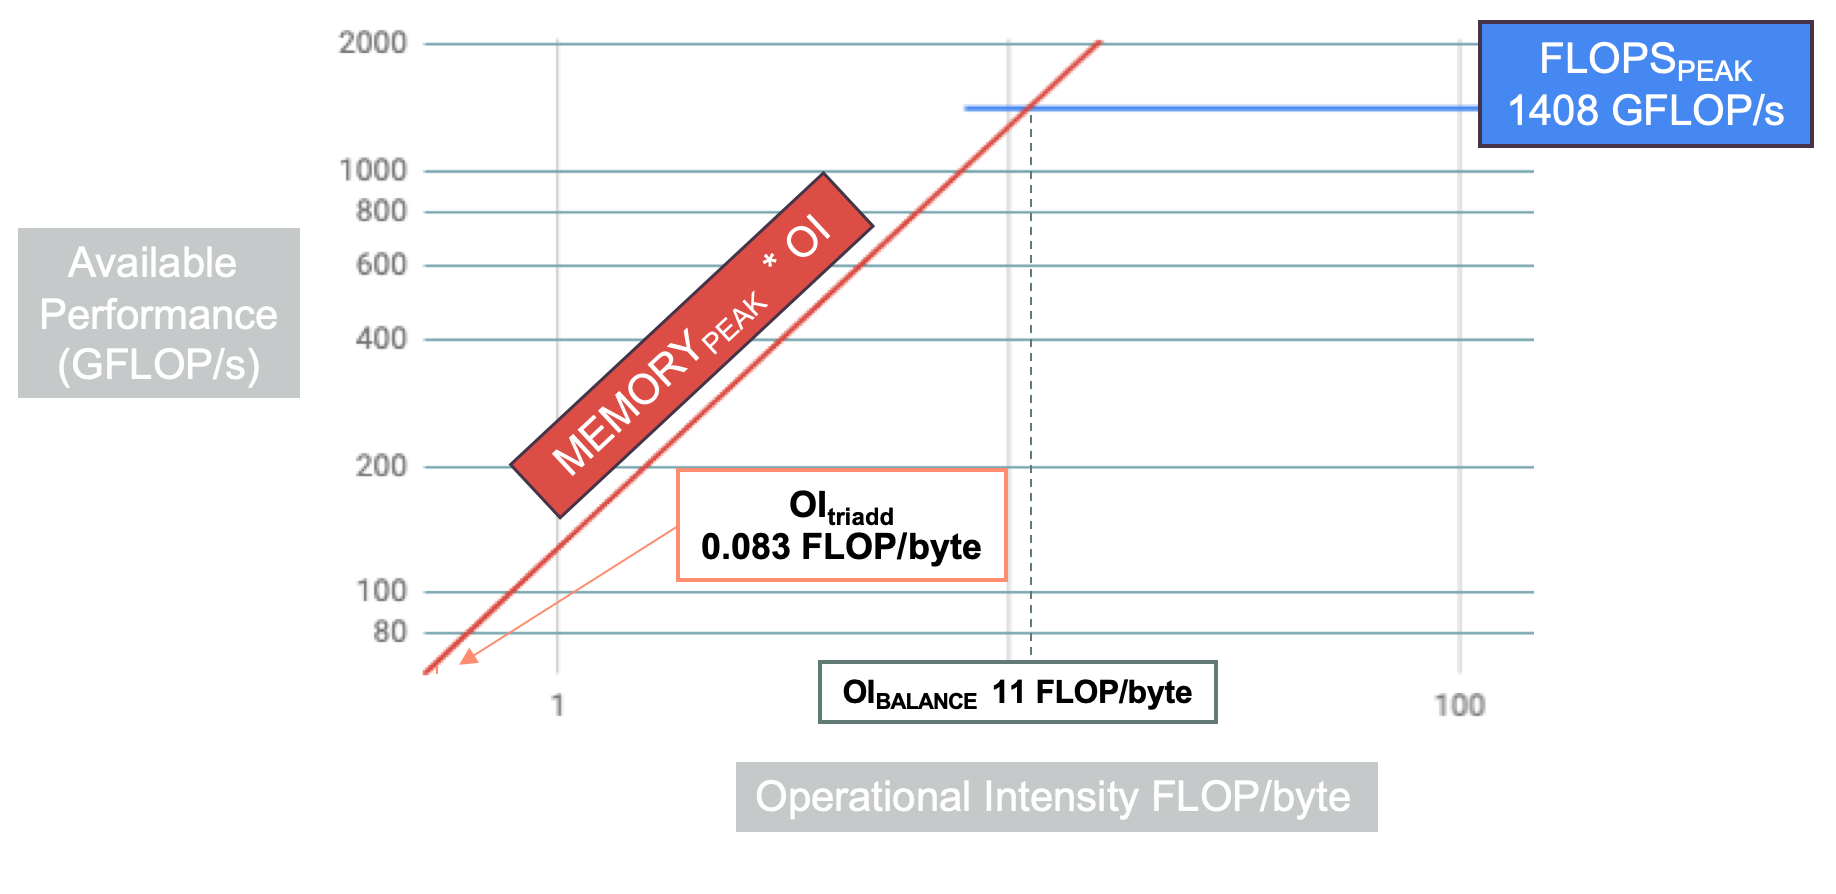
\includegraphics[width=10cm]{images/roofline_stream.png}
    \caption{\label{pic:roofline_stream} Modèle du \textit{Roofline} appliqué à la fonction \textit{triadd} du benchmark \textit{Stream} et un processeur Xeon Skylake 6148.}
\end{figure}



\subsubsection{Simple Memory Model} 
%%%%%%%%%%%%%%%%%
L'analyse de la fonction avec le modèle du \textit{roof line} indique que sur l'architecture ciblée, la performance du code sera limité par la performance de la bande passante.
A chaque itération de boucle, deux opérations doivent être réalisées, une addition et une multiplication. 

Une fois assuré que les performances de l'application sont limitées par le système mémoire, le Simple Memory Model peut être appliqué. Dans notre éxpérimentation, nous utilisons trois matrices de 19.6 GB ($3 \times 10^9 \times sizeof(double)$). Pour une exécution optimale, le bus mémoire devrait être utilisé pour charger une fois les deux matrices en lectures (matrices B et C)  et pour l'écriture de la matrice A. Le traffic mémoire total serait alors de 58.8 GB. En utilisant les résultats mesurés lors de l'étape 2, on peut estimer le temps optimale pour l'exécution de cette fonction: $\text{TEMPS}_{optimal} = \frac{58.8}{128} = 0.56$ seconde.









%%%%%%%%%%%%%%%%%%%%%%%%%%%%%%%%%%%%%%%%%%%%%%%%%%%%%%%%%%%%%%%%%%%%%%%%%%%%%%%%%%%%%%%%
%%%%%%%%%%%%%%%%%%%%%%%%%%%%%%%%%%%%%%%%%%%%%%%%%%%%%%%%%%%%%%%%%%%%%%%%%%%%%%%%%%%%%%%%
%%_______ .___________.    ___      .______    _______                      _  _      %%
%%|   ____||           |   /   \     |   _  \  |   ____|                   | || |     %%
%%|  |__   `---|  |----`  /  ^  \    |  |_)  | |  |__          ______      | || |_    %%
%%|   __|      |  |      /  /_\  \   |   ___/  |   __|        |______|     |__   _|   %%
%%|  |____     |  |     /  _____  \  |  |      |  |____                       | |     %%
%%|_______|    |__|    /__/     \__\ | _|      |_______|                      |_|     %%
%%%%%%%%%%%%%%%%%%%%%%%%%%%%%%%%%%%%%%%%%%%%%%%%%%%%%%%%%%%%%%%%%%%%%%%%%%%%%%%%%%%%%%%%
%%%%%%%%%%%%%%%%%%%%%%%%%%%%%%%%%%%%%%%%%%%%%%%%%%%%%%%%%%%%%%%%%%%%%%%%%%%%%%%%%%%%%%%%

%%%%%%%%%%%%%%%%%%%%%%%%%%%%%%%%%%%%%%%%%%%%%%%%%%%%%%%%%%%%%%%%%%%
\section{Étape 4: Sélection de la plate-forme}
%%%%%%%%%%%%%%%%%%%%%%%%%%%%%%%%%%%%%%%%%%%%%%%%%%%%%%%%%%%%%%%%%%%


%%%%%%%%%%%%%%%%%
\subsection{Motivations et objectifs}
%%%%%%%%%%%%%%%%%


Dans l'utilisation d'une plate-forme Exascale, la majorité des lignes de codes seront encore exécutés sur des processeurs standard. Ces zones de codes doivent être identifiées, portées et optimisées sur des architectures optimisées pour leur exécution. Par exemple, une fonction réalisant de la compression de données pourra être exécutée sur un accélérateur à bas coût spécialisé pour cette tâche. Le budget ainsi économisé pour être réinvesti dans d'autres accélérateurs plus puissant et performant pour les parties critiques du code. 

L'objectif de cette étape est d'aider à la sélection des plate-formes adaptées aux kernels identifiés dans l'étape précédente.


%%%%%%%%%%%%%%%%%
\subsection{Le coût}
%%%%%%%%%%%%%%%%%

Le coût de l'architecture ciblé est important, mais aussi celui de la solution globale. Beaucoup de paramètres entrent en jeu dans le calculs de prix total appelé coût total de possession ou $\text{TCO}$. Il prend en compte tout les coûts engendrés par le centre de données durant son cycle de vie. Le budget pour la construction du premier centre Exascale Européen est de 500 millions d'euros \cite{SergiGirona2018}.

\subsubsection{Le prix du matériel} 
Le  prix des accélérateurs et du matériels nécessaire à la construction du supercalculateur une part significative dans le calcul du coût (\textbf{todo: une idée ?}). En fonction du prix de l'accélérateur, une solution moins performante pourra lui être préféré. Même si d'autres raison interviennent comme la complexité de programmation, le prix des cartes FPGA est une raison majeure de leur faible utilisation dans les clusters du Top500.

\subsubsection{La consommation électrique}
La majorité des data center ont des lignes électriques déjà construite permettant d’acheminer une quantité limité de courant. La consommation électrique de la plate-forme finale est devenue un critère très important dans le choix du matériel. La consommation des centres de données est un réel investissement qui doit être mesuré et anticipé lors de l'achat du matériel. Un supercalculateur consommant 10 Mwatt engendrera un facture plusieurs millions d'euros chaque année. Le prix de l'électricité et l'enveloppe énergétique disponible pour le calcul dépend de la localisation du centre de données. La chaleur de la zone géographique de son installation impactant le refroidissement nécessaire. Ainsi en 2018, Microsoft a décidé de couler ses serveurs au fond de l'océan pour profiter d'un refroidissement gratuit \cite{ChristineHall2018}.

\subsubsection{La taille du centre de donnée} 
Souvent les centre de données sont déjà existant et la taille disponible pour la création d'un supercalculateur ou l'ajout de nouveaux serveurs est une contrainte forte. Certaines solutions prenant plus ou moins de place pour être installées, le ratio $\frac{flop}{m^2}$ peut alors être calculé pour évaluer la densité des serveurs pour s'adapter aux contraintes du lieu. Si le bâtiment doit être construit pour accueillir le supercalculateur, son coût doit entrer dans le calcul de la solution finale.




%%%%%%%%%%%%%%%%%
\subsection{La performance}
%%%%%%%%%%%%%%%%%

\subsubsection{Performance du kernel}
Le choix de l'accélérateur prend en considération la performance qu'aura l'application lorsque le kernel y sera porté. Les étapes 1 et 2 ont permis d'établir les performances d'une architecture. L'étape 3 à elle permis de modéliser les performances d'un kernel en fonction de la performance de la bande passante passante en calculant $\text{TEMPS}_{optimal}$, le temps optimal pour exécuter ce kernel sur l'architecture considérée.

\subsubsection{Efficacité énergétique}
En comparant son intensité opérationnelle  $\text{OI}_{kernel}$ et l'équilibre arithmétique de la plate-forme $\text{EQUILIBRE}_{plateforme}$ il est possible d'estimer la pertinence d'un accélérateur pour un kernel. Des valeurs proches, indiquent que l'architecture ciblée est adaptée au code étudié et que l'accélérateur choisi aura un meilleur rendement énergétique. Un code faisant peu de calculs flottant ne nécessitera pas l'utilisation de coeurs complexes réalisant plusieurs dizaines de flop par cycle. Bien que non utilisés, ces composants impactent le prix de la solution mais aussi sa consommation électrique. Une grande part des centre de données consomment aujourd'hui la totalité de l'électricité disponible. Ces supercalculateurs doivent alors se tourner vers des solutions plus efficace énergétiquement.


\subsubsection{Difficulté du portage}
Le code de l'application  et les transformations nécessaires doivent être pris en compte car il peut avoir un impact sur les performances ou financier. Le travail de portage de l'application sur une nouvelle architecture doit être mesuré. Suivant l'architecture choisie, il faudra peut être coder l'application avec un nouveau langage. Le temps $\text{TEMPS}_{optimal}$, pour exécuter l'application considère que l'application utilise de façon optimale l'architecture. Cependant pour atteindre ces performances, le kernel peut nécessiter d'être optimiser et certaines peuvent être très difficile à implémenter sur des codes existants. Certaines optimisations nécessitent une réelle expertise du domaine et du matériel envisagé. Lorsqu'une optimisation est choisi d'être implémentée le risque de ne pas parvenir à obtenir les performances espérées doit lui aussi être mesuré. Il peut arriver qu'une optimisation moins performante soit préférée car la transformation du code est plus facile. Le temps et le nombre de programmeurs nécessaires à son implémentation entre aussi en considération dans le prix de la solution


\subsubsection{Performance des applications }
La performance du kernel a un impact financier car s'il est exécuté plus rapidement, d'autres applications pourront alors accéder à la plate-forme. Les clients de supercalculateurs ont généralement un budget fixe et de multiples applications à exécuter. Ils cherchent alors à optimiser l'utilisation des ressources informatiques par les différents codes. Bien que l'on considère de porter individuellement chaque kernel sur un accélérateur le plus adapté, il faut aussi prendre en considération le reste de l'application mais aussi celle des autres utilisateurs. Si une seule des applications exécutée par l'utilisateur ne bénéficie des performances d'un accélérateur, il serait plus pertinent d'opter pour un accélérateur plus "globale". 


%%%%%%%%%%%%%%%%%
\subsection{Application au benchmark Stream et au processeur Intel Xeon 6148}
%%%%%%%%%%%%%%%%%
 \textbf{TODO:} l'application a telle un sens alors qu'on compare qu'un seul matériel ? Est ce que pour cette étape on le compare à un accélérateur NEC ou GPU ?

%Nous continuons l'analyse du benchmark Stream et du processeur Intel Xeon 6148 débutée dans les étapes précédentes. Cette application prend pour postulat que ce processeur est envisagé pour le portage du kernel. Lors de l'étape 3, l'intensité arithmétique de la fonction tri-add avait été mesuré à $12\ bytes/flop$. Pour estimer si le processeur envisagé est \textbf{bon?} pour y porter cette fonction, son équilibre arithmétique doit être calculé. \textbf{TODO INVERSE} Le processeur Intel Xeon 6148 possède une instruction FMA, les deux opérations de la boucle (addition et multiplication) peuvent se faire en une seule instruction. $3 \times 8 = 24$ éléments en double précision, ce qui correspond à 192 bytes. L'intensité arithmétique de cette fonction est de $ \frac{192}{32} = 6\ byte/flop$. 









\iffalse 
%%%%%%%%%%%%%%%%%%%%%%%%%%%%%%%%%%%%%%%%%%%%%%%%%%%%%%%%%%%%%%%%%%%%%%%%%%%%%%%%%%%%%%%%
%%%%%%%%%%%%%%%%%%%%%%%%%%%%%%%%%%%%%%%%%%%%%%%%%%%%%%%%%%%%%%%%%%%%%%%%%%%%%%%%%%%%%%%%
%%_______ .___________.    ___      .______    _______                      _____     %%
%%|   ____||           |   /   \     |   _  \  |   ____|                   | ____|    %%
%%|  |__   `---|  |----`  /  ^  \    |  |_)  | |  |__          ______      | |__      %%
%%|   __|      |  |      /  /_\  \   |   ___/  |   __|        |______|     |___ \     %%
%%|  |____     |  |     /  _____  \  |  |      |  |____                     ___) |    %%
%%|_______|    |__|    /__/     \__\ | _|      |_______|                   |____/     %%
%%%%%%%%%%%%%%%%%%%%%%%%%%%%%%%%%%%%%%%%%%%%%%%%%%%%%%%%%%%%%%%%%%%%%%%%%%%%%%%%%%%%%%%%
%%%%%%%%%%%%%%%%%%%%%%%%%%%%%%%%%%%%%%%%%%%%%%%%%%%%%%%%%%%%%%%%%%%%%%%%%%%%%%%%%%%%%%%%
\fi



%%%%%%%%%%%%%%%%%%%%%%%%%%%%%%%%%%%%%%%%%%%%%%%%%%%%%%%%%%%%%%%%%%%
\section{Étape 5: Portage et optimisation du code}
%%%%%%%%%%%%%%%%%%%%%%%%%%%%%%%%%%%%%%%%%%%%%%%%%%%%%%%%%%%%%%%%%%%
 

%%%%%%%%%%%%%%%%%
\subsection{Motivations et objectifs}
%%%%%%%%%%%%%%%%%


Lors de l'étape 4, une plate-forme a été choisie en fonction de plusieurs critère pour y porter les kernels. L'étape 5 s'occupe du portage du code et de la validation du modèle de performance. Nous montrons comment les outils développés lors de cette thèse sont crucial pour l'analyse de performance. Lorsque le code n'atteint pas les performances espérées, nous proposons un cheminement pour trouver d'où vient ce problème et comment le régler. 


%%%%%%%%%%%%%%%%%
\subsection{Portage de l'application}
%%%%%%%%%%%%%%%%%


\subsubsection{Premier développement}
%%%%%%%%%%%%%%%%%
Une fois la plate-forme choisie il faut appliquer les transformations du code nécessaires pour pouvoir y exécuter les kernels. L'effort nécessaire pour adapter le code à cette nouvelle architecture a dû être évalué lors de l'étape précédente. Le portage du code peut nécessiter un changement de langage de programmation ou de paradigme de programmation.
Si possible, il est important d'utiliser des librairies déjà optimisées pour espérer atteindre les performances crêtes de l'application. De plus, les constructeurs de la plate-forme peuvent avoir développé des librairies (NVIDIA, NEC) pouvant être casi-optimale et qui nécessitent une grande expertise pour être développées.




\subsubsection{Vérification du modèle de performance}
%%%%%%%%%%%%%%%%%

Lors de l'étape 4, un modèle de performance du kernel à été établi (voir paragraphe \ref{sec:smm}). Pour s'assurer des performances du kernel une fois porté, il faut comparer ses performances mesurées avec celles établies par le modèle. Comparer la performance théorique à la performances réelle permet de valider les bonnes performances ou, dans le cas contraire, de les quantifier par rapport à l'optimum théorique $\text{TEMPS}_{optimal}$. Nous avions alors préféré calculer $\text{TEMPS}_{optimal}$ à partir des performances maximales $\text{MEMORY}_{max}$ atteintes par nos benchmark.

Pour mesurer le temps d'exécution du kernel, $\text{TEMPS}_{mesure}$, nous proposons d'utiliser la fonction \textit{gettimeofday ()} \cite{Linux}. Cette fonction est disponible sur la totalité des système linux et permet de récupérer l'heure actuelle avec une précision allant jusqu'à la microseconde. Le but de la méthodologie présentée est de porter les codes sur de nouvelles architectures. Baser l'analyse de performance sur des compteurs matériels trop complexes aurait réduit la portabilité de notre démarche. On peut mesurer  $\text{TEMPS}_{mesure}$ en plaçant deux appels à la fonction \textit{gettime} présentée dans l'\autoref{lst:gettime}, avant et après le kernel.


\begin{lstlisting}[language=c,caption=Fonction utilisée pour lire la date actuelle avec une précision allant jusqu'à la microseconde,label={lst:gettime}, 
  basicstyle=\footnotesize, frame=tb,
  xleftmargin=.065\textwidth, xrightmargin=.065\textwidth]
double gettime()
{
  struct timeval tp;
  struct timezone tzp;
  int i;
  i = gettimeofday(&tp,&tzp);
  return ( (double) tp.tv_sec + (double) tp.tv_usec * 1.e-6 );
}
\end{lstlisting}

Si $\text{TEMPS}_{mesure}$ est proche de $\text{TEMPS}_{optimal}$ alors le kernel est proche d'avoir des performances optimale. En effet, dans le cas de code limité par la bande passante, notre modélisation permet de calculer le temps minimale pour exécuter le kernel, en calculant le temps nécessaire pour déplacer le jeu de données de la mémoire au processeur. Pour un même algorithme il est théoriquement impossible d'exécuter le kernel plus rapidement. La mesure $\text{TEMPS}_{optimal}$ permet d'avoir un objectif de performances à atteindre et de savoir quand le travail d'optimisation est terminé en mesurant simplement son temps d'exécution. Malheureusement, la majorité des applications ont du mal à atteindre cette performance et doivent avoir recourt à des technique d'optimisation de localité pour minimiser le nombre de relecture du jeu de donnée. 




%%%%%%%%%%%%%%%%%
\subsection{Profilage des performances}
%%%%%%%%%%%%%%%%%

Si la mesure de $\text{TEMPS}_{mesure}$  a montrer que le code était inefficace il est alors nécessaire d'en comprendre la raison. Pour cela, le programmeur doit avoir des outils à sa disposition lui permettant de comprendre la cause de ces performances. Même si l'analyse par le modèle du \textit{roofline} a montré que la performance maximale atteignable était limitée par la bande passante mémoire, le proceseur peut lui aussi dégrader les performances (mauvaise compilation, dépendances de données, \textit{cache misses}). Utilisés de façon méthodique les deux outils présentés dans cette thèse, \textit{OProfile++} et \textit{YAMB}, permettent de répondre à beaucoup de question et mener à bien le travail d'optimisation du code dont une vue d'ensemble est proposée sur la \autoref{pic:analyse_bigpicture}.

\begin{figure}
    \center
    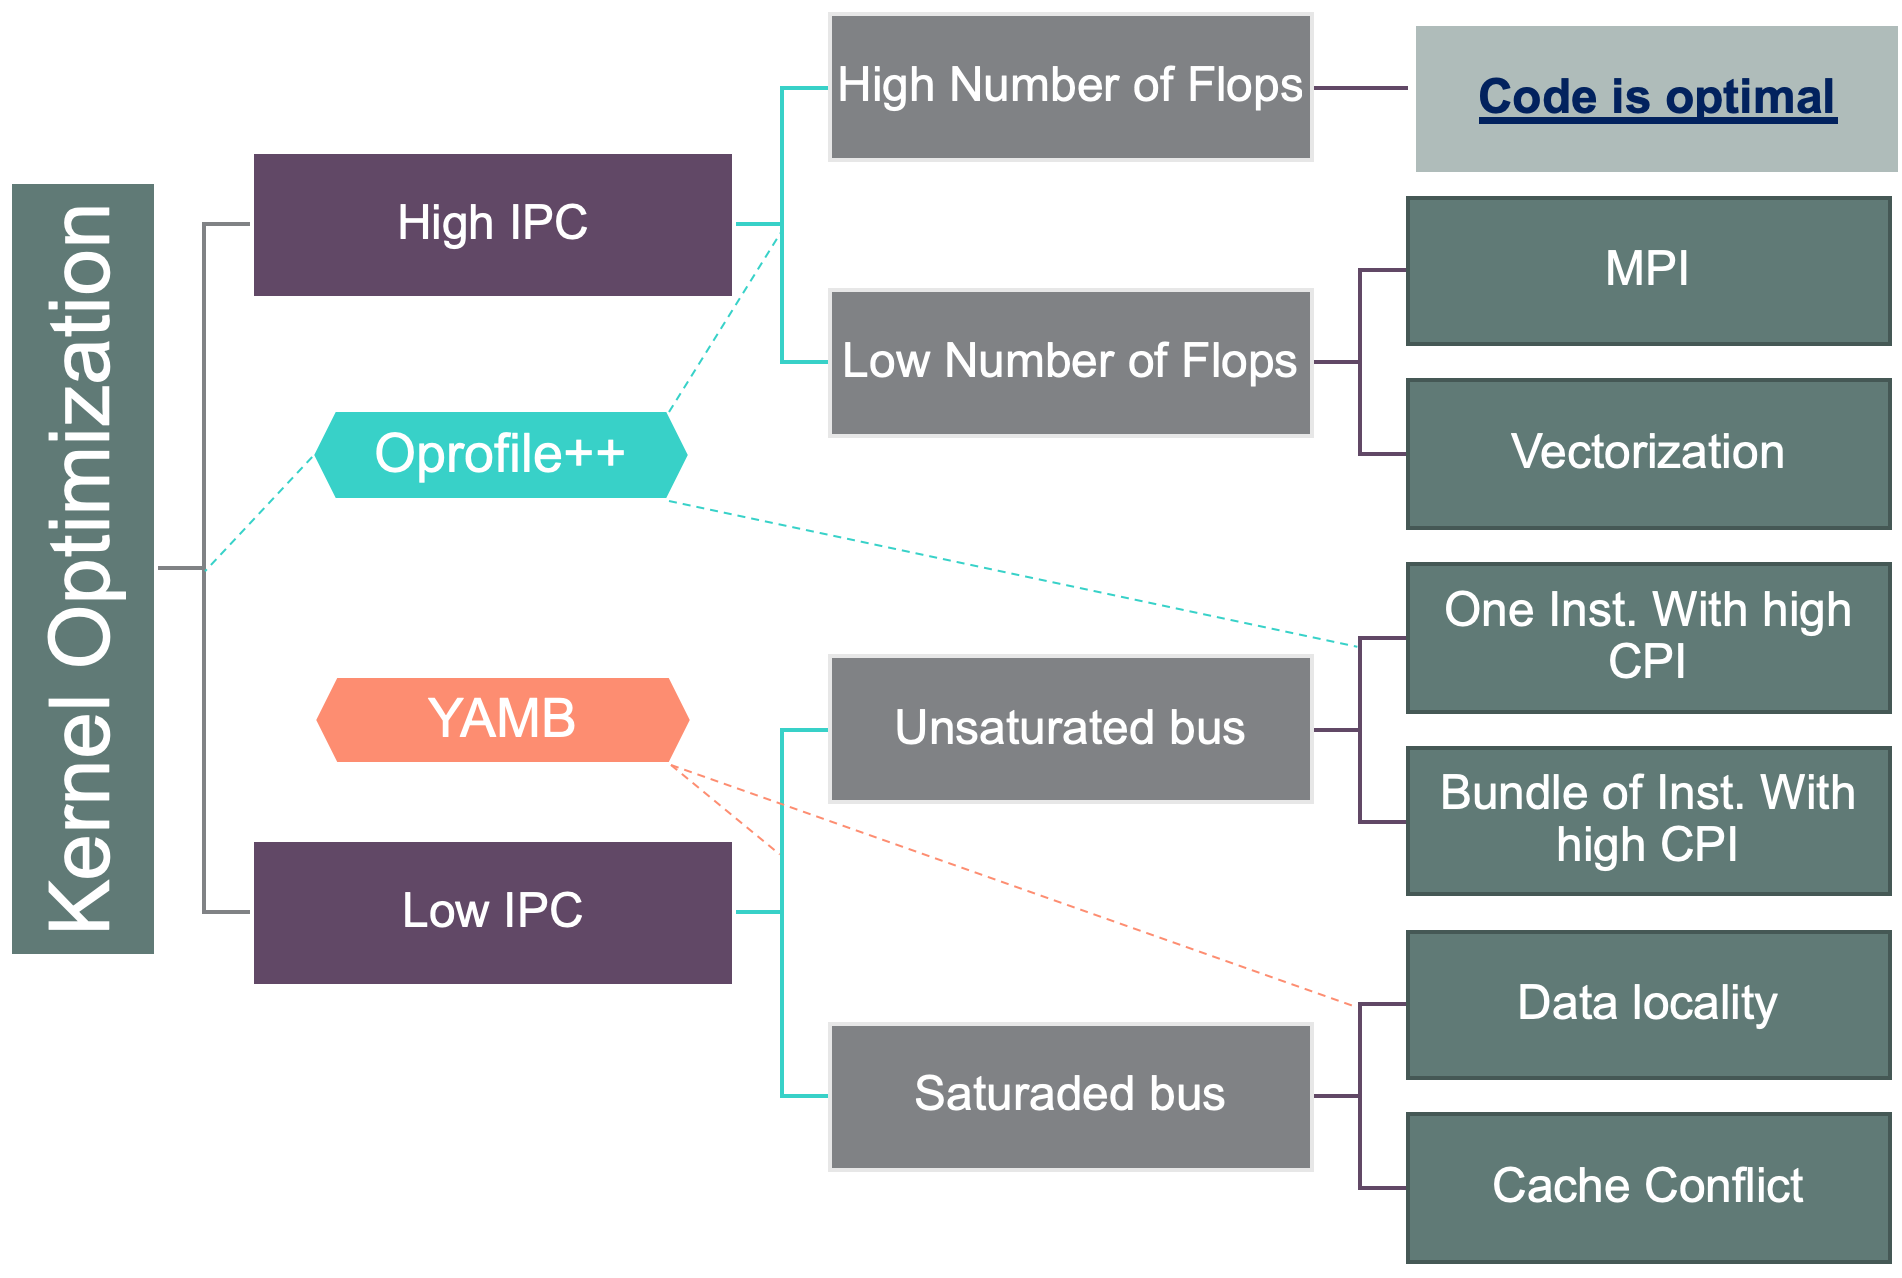
\includegraphics[width=11cm]{images/analyse_bigpicture.png}
    \caption{\label{pic:analyse_bigpicture} Flux de travail pour l'utilisation des outils \textit{Oprofile++} et \textit{YAMB}. La première étape est de mesurer l'IPC du kernel pour déterminer si le processeur ou la mémoire limite les performances. En fonction des observations amenées par les outils, des réponses différentes sont proposées au programmeur pour optimiser son code.}
\end{figure}



\subsubsection{Profilage de la mémoire}
%%%%%%%%%%%%%%%%%
Si la performance est inférieure aux attentes, la première question à se poser est de savoir si le bus mémoire est saturé. Pour y répondre, nous proposons l'outil YAMB qui affiche l'activité du bus mémoire (lecture, écriture et utilisation totale). Pour confirmer sa saturation, il est nécessaire d'avoir caractérisé la performance du bus mémoire dans la première étape. Si le bus n'est pas saturé, la mauvaise performance est due à une autre pathologie. Si le bus est bien saturé et comparer les ratio de lecture/écriture avec ceux mesurée lors de l'étape 3 présentée dans la \autoref{sec:smm}. Grâce à ces ratios, on peut déterminer si le jeu de donnée est lu plusieurs fois, et si des techniques de \textit{blocking} pour améliorer la localité dans la mémoire cache doivent être utilisées. Si le ratio n'est pas celui attendu, c'est parce que le nombre de lectures est plus élevé que prévu. Un mauvais ratio peut provenir d'un nombre de lectures plus élevé que prévu. Ceci est causé par un large éventail de problèmes potentiels, par exemple, des conflits dans le cache, la lecture de données inutiles, une décomposition incorrecte des données ou des structures de mémoire inappropriées. Il est très rare qu'un code écrive plus qu'il ne devrait.





\subsubsection{Profilage du processeur}
L'exécution de l'assembleur peut être suivie avec l'outil \textit{Oprofile++} (voir \autoref{sec:oprofile++}). Il permet d'extraire le code assembleur et d'y agrémenter les compteurs de cycles comme le montre l'\autoref{lst:oprofileex}. L'outil aide pour trouver si des motifs d'instructions sont plus long à exécuter que d'autres, pouvant être expliqué par une dépendance entre les données ou une donnée non présente dans la mémoire cache au moment requis. 
Si des instructions de calculs flottant sont responsables d'un grand nombre de cycle, on peut vérifier le bon fonctionnement du processeurs pour celles ci grâce au générateur de kernels (\autoref{sec:kg}). 


\begin{lstlisting}[language={},caption=L'outil \textit{Oprofile++} permet d'extraire le code assembleur et d'y associer le compteur de cycle,label={lst:oprofileex}, 
  frame=tb]
================================================================
Analysis from the app name (horner1_long) hot spot from the symbole name (f1(double)) which takes 50.1878% 
================================================================
CYCLES       INSTS      ADDRESS    disassembly
----------------------------------------------------------------
     5           11      401be0    vmovupd 0xd1b8(%rip),%ymm1
    39           79      401bf0    vfnmadd231pd 0xd1c7(%rip),%ymm11,%ymm1
     3           14      401bf9    vfmadd213pd %ymm2,%ymm11,%ymm1
...
   760         1652      401c3e    cmp    %eax,%edx
    48           99      401c40    jb     401be0 <_Z8range_f1ddi+0xa0>
----------------------------------------------------------------
LOOP from 401c40 to 401be0  size= 96 sum(cycles)= 2287 
     IPC= 2.12462 cycles/LOOP= 10.3548 flop/cycle = 1.42 
----------------------------------------------------------------
\end{lstlisting}





%%%%%%%%%%%%%%%%%
\subsection{Optimisations: méthodologie d'analyse et d'optimisation}
%%%%%%%%%%%%%%%%%

\textbf{TODO: } écrire une section sur comment optimiser un code en suivant toutes les branches de la figure, et en proposant des optimisations

\begin{figure}
    \center
    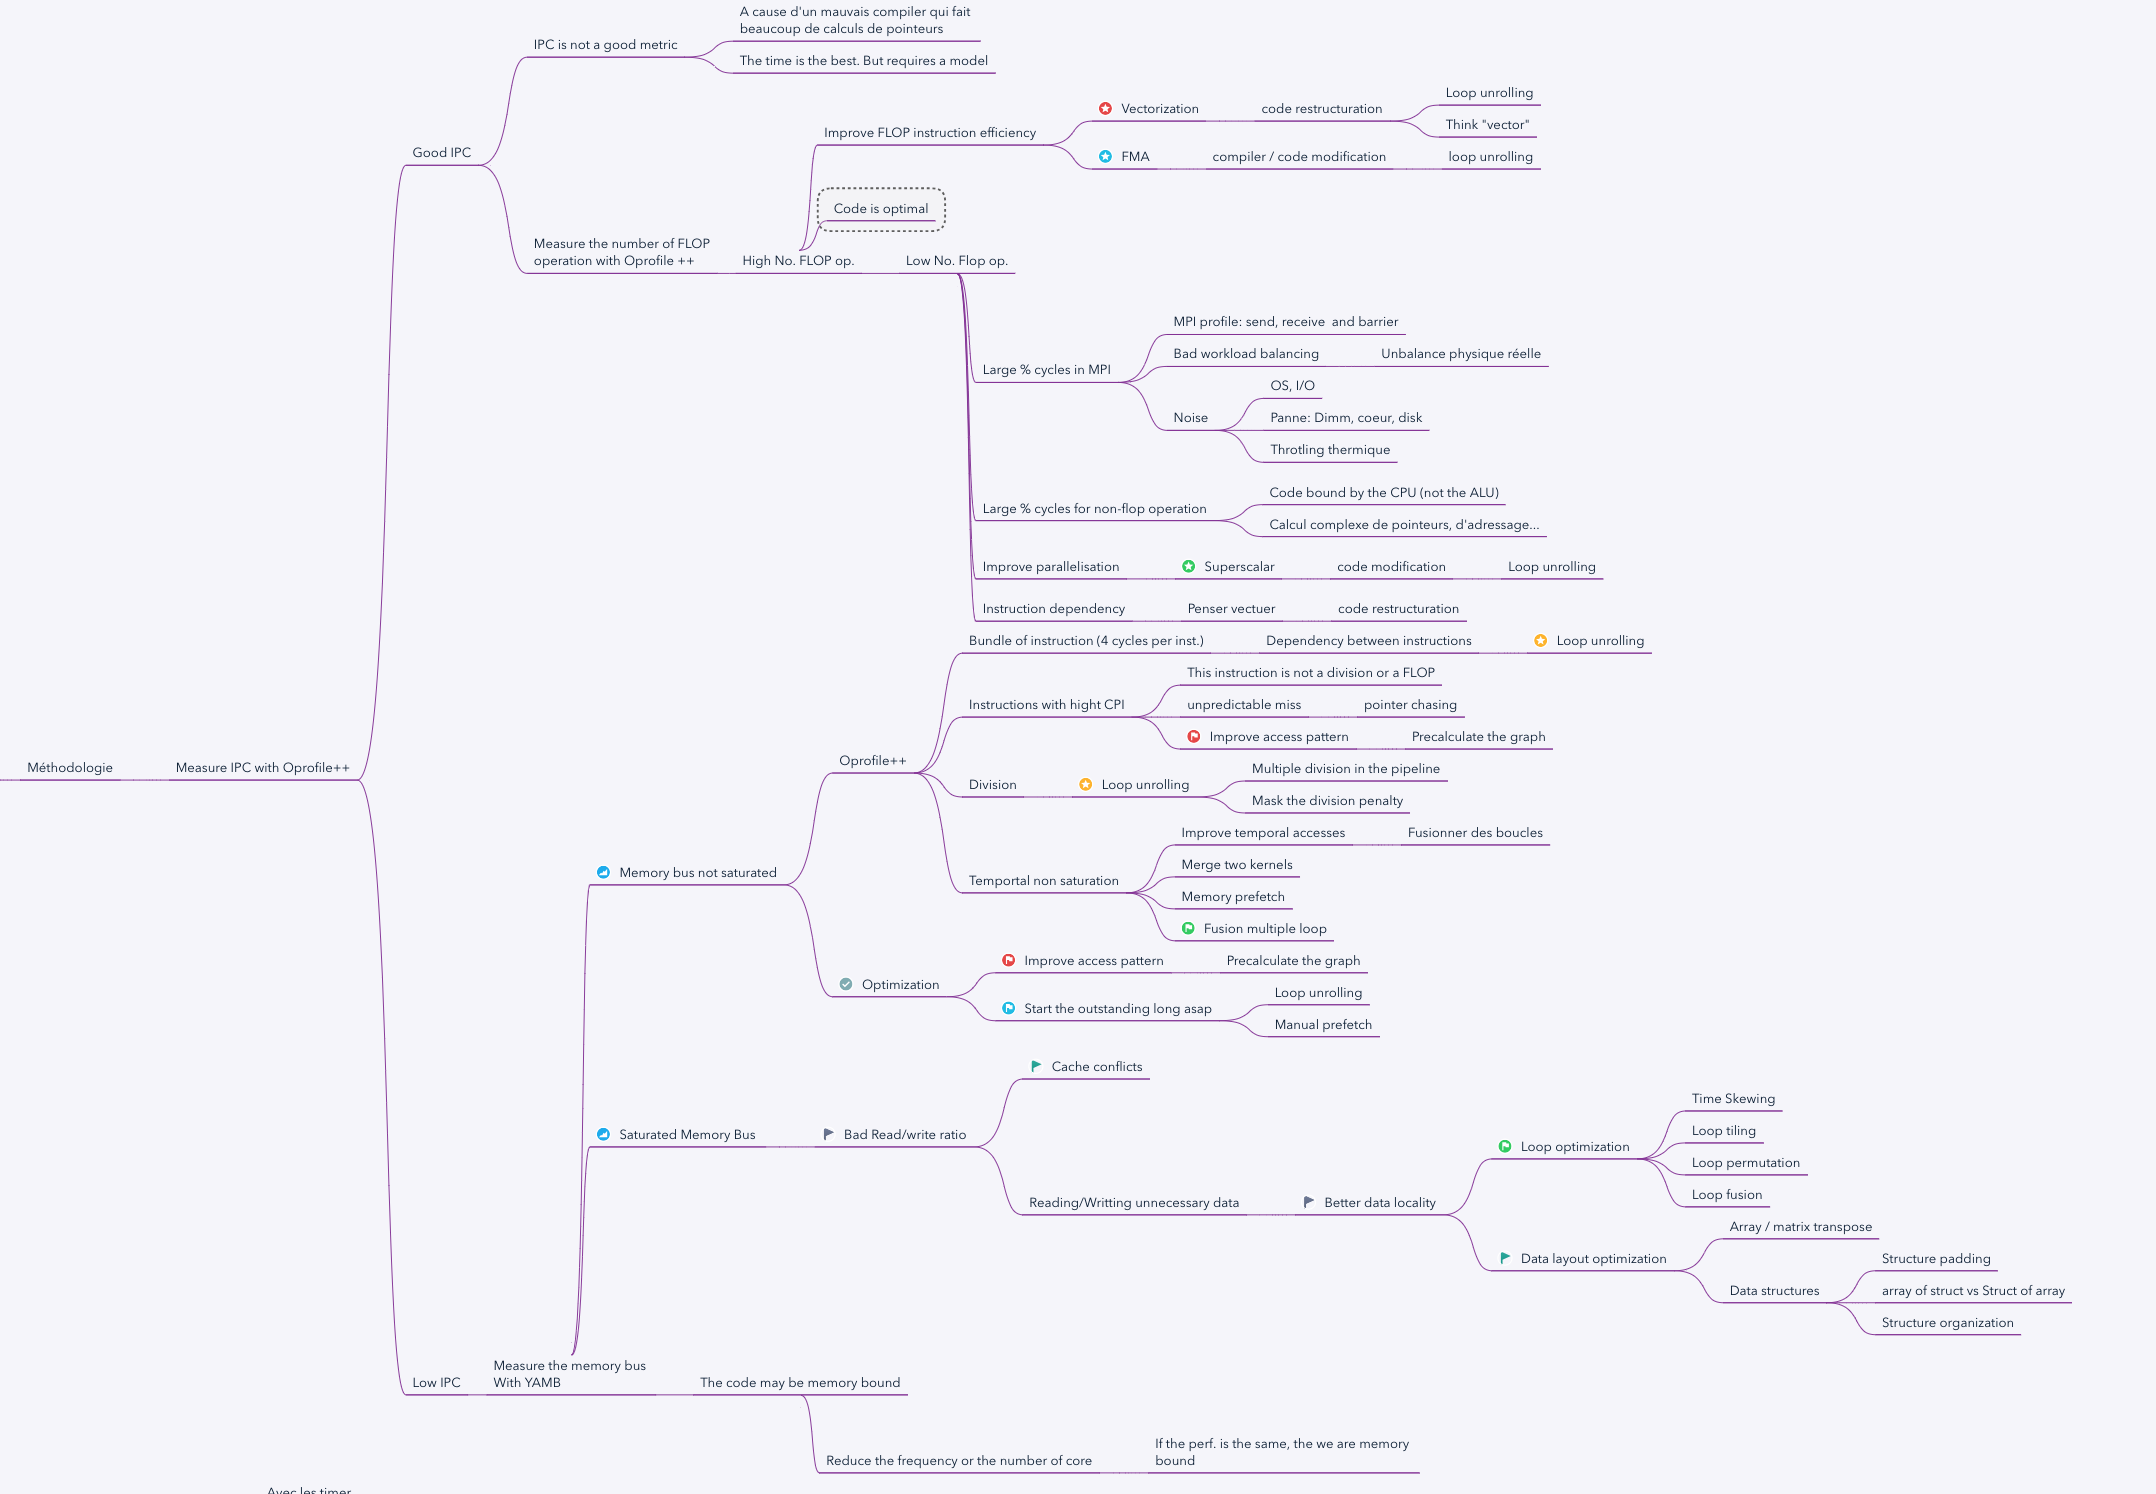
\includegraphics[width=18cm]{images/methodologie_optimisation.png}
    \caption{\label{pic:methodologie_optimisation} \textbf{TODO: } écrire une section sur comment optimiser un code en suivant toutes les branches de la figure, et en proposant des optimisations}
\end{figure}



%%%%%%%%%%%%%%%%%
\subsection{Application au benchmark \textit{Stream}}
%%%%%%%%%%%%%%%%%

Nous appliquons notre méthodologie sur le benchmark Stream fonctionnant sur un processeur Intel Skylake. Cet exercice nous permet de montrer que même sur un code aussi simple, apparemment optimal, notre analyse nous permet de comprendre sa performance et de l'optimiser.


\subsubsection{Vérification du modèle SMM}
%%%%%%%%%%%%%%%%%

Nous avons montré précédemment que la performance du code était limité par la bande passante mémoire. Nous avons appliqué notre modèle de performance SMM et déterminé $\text{TEMPS}_{optimal} = \frac{58.8}{128} = 0.56$ seconde. En utilisant la fonction présenté dans l'\autoref{lst:gettime} nous mesurons $\text{TEMPS}_{mesure} = 0.79$ seconde.

L'application n'est donc pas optimale. Ceci est également validé par le résultat du benchmark Stream qui annonce une bande passante mémoire de 80,13 Go/sec. Pour comprendre ce résultat, nous avons utilisé YAMB pour vérifier que le bus mémoire était bien saturé. Le graphique de la \autoref{fig:stream_before} nous montre que le bus mémoire est utilisé au maximum de son potentiel de 104 GB/s. La saturation du bus n'est donc pas la cause de la mauvaise performance du noyau. Il est alors nécessaire de regarder les rapports lecture/écriture. La \autoref{fig:stream_before} montre cette répartition : 26 Go/s en écriture pour 78 Go/s en lecture, puis un total de 104 Go/s, ce qui correspond à un ratio de 1 écriture pour 3 lectures. Bien que nous nous attendions à un ratio d'une écriture pour deux lectures, ce ratio exact d'une écriture pour trois lectures n'est pas une coïncidence. Un vecteur entier est lu alors qu'il ne devrait pas l'être.

\begin{figure}[htb]
{
\centering
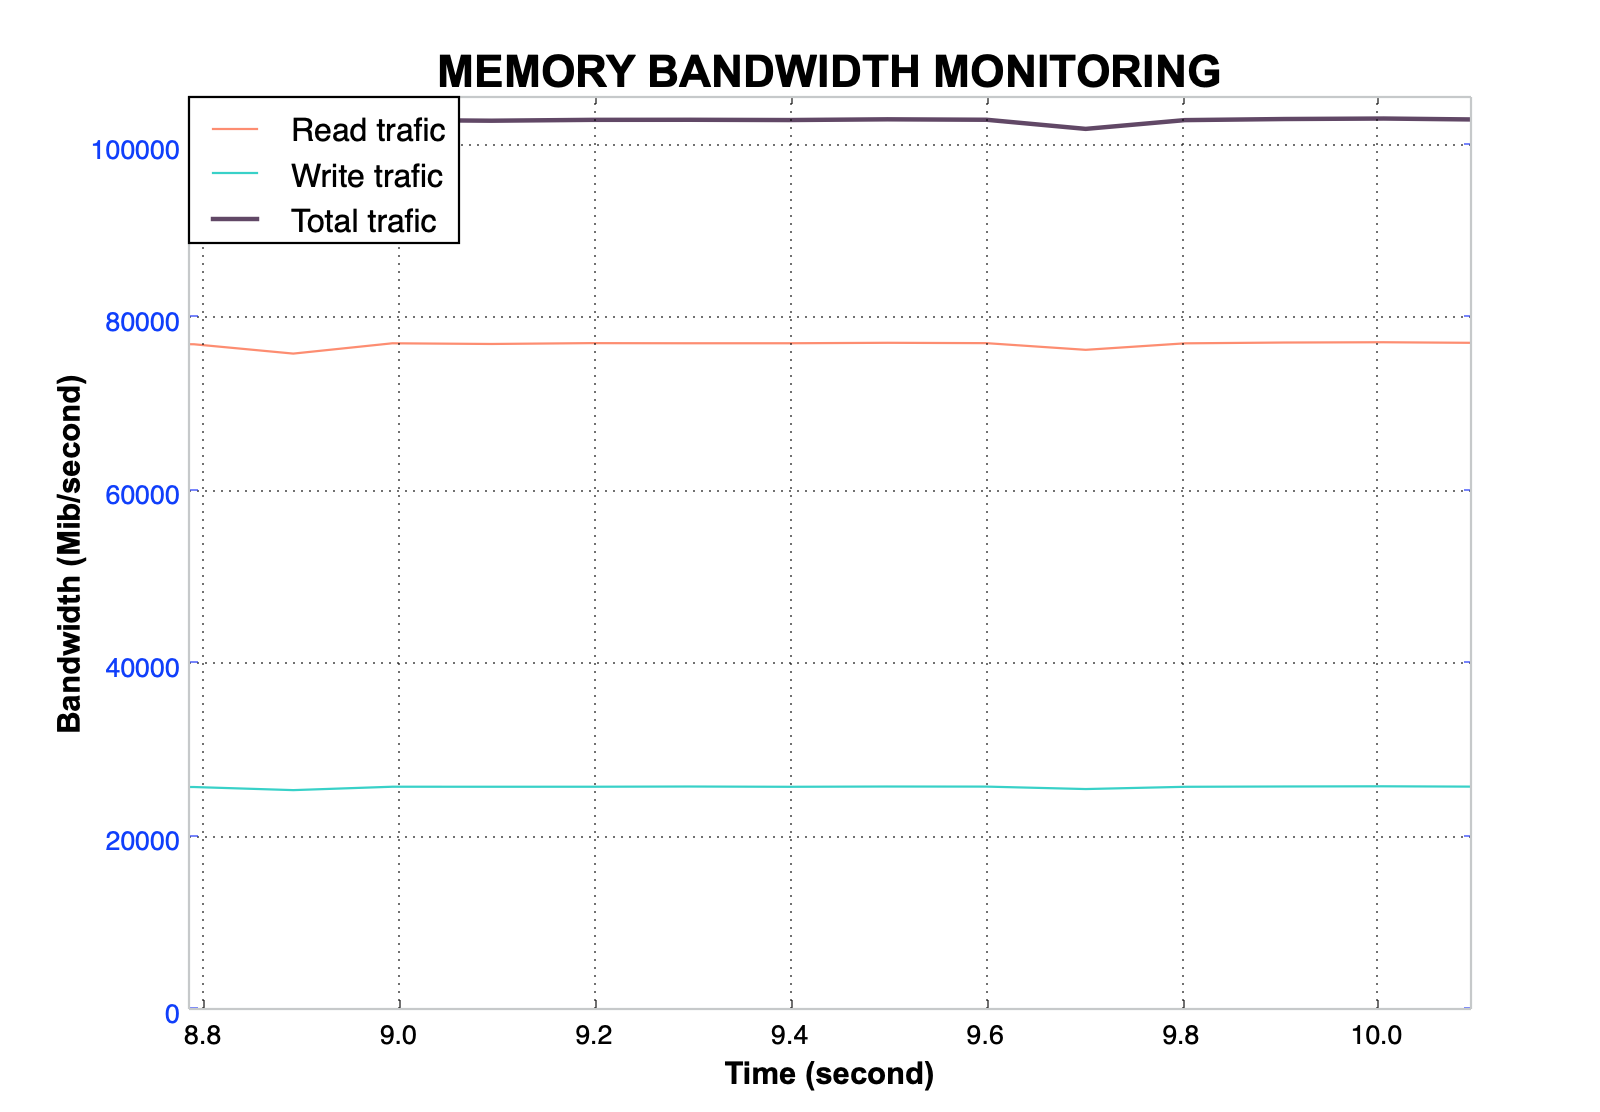
\includegraphics[width=0.80\textwidth]{images/stream_before.png}
\caption{Prolie mémoire donné par l'outil YAMB pour plusieurs exécution de kernel \textit{triadd} du benchmark \textit{Stream}. }\label{fig:stream_before}
}
\end{figure}



\subsubsection{Optimisation du kernel \textit{triadd}}
%%%%%%%%%%%%%%%%%

Les deux vecteurs B et C doivent nécessairement être rouges une fois. La lecture supplémentaire provient du vecteur en écriture A. Ce comportement est dû au processeur qui, avant d'écrire une donnée, charge la ligne de cache correspondante pour la mettre à jour. Cependant, le kernel étudié a la particularité d'écrire toute la ligne de cache, les données initialement présentes n'ayant aucune valeur utile. Une option peut être utilisée avec le compilateur Intel (ICC) pour contourner ce comportement : \textit{-qopt- streaming-stores=always}. Cette option permet au CPU d'écrire toute la ligne de cache sans avoir à la charger.


\subsubsection{Performance du kernel optimisé}
%%%%%%%%%%%%%%%%%

Nous avons compilé \textit{Stream} avec l'option \textit{-qopt- streaming-stores=always} et mesuré le temps et la bande passante de la même manière que pour la première exécution. Les résultats sont résumés dans le \autoref{table:stream_res}. Le temps passé dans le noyau est de 0,59 seconde, beaucoup plus proche du maximum théorique de 0,56 seconde. En analysant la bande passante mémoire, on constate que le rapport lecture/écriture est maintenant de 2 pour 1, les données échangées étant de 34 Go/s en mode écriture pour 68 Go/s en mode lecture. Le total approche la limite du bus, maintenant 102GB/s.

 \renewcommand{\arraystretch}{1.2}
    \setlength{\tabcolsep}{8pt}
    
    \begin{table}[htbp]
        \centering

        \caption{Performance du kernel \textit{triadd} du benchmark \textit{Stream} avant et après optimisation. Le temps (seconde) après optimisation est proche de l'optimum théorique $\text{TEMPS}_{optimal}$  calculé à 0,56 sec. L'utilisation du bus mémoire est approximativement la même entre les deux versions du code (104 et 102 Go/s). L'option de compilation optimise le rapport lecture/écriture (Go/s) et améliore les performances du code de 25\%.}

            \begin{tabular}{l|c|c|c|c|c|}
            \cline{2-6}
                                            & $\text{T}_{mesure} (s)$ & Stream  (GB/s) & $\text{YAMB}_{read}$ (GB/s) & $\text{YAMB}_{write}$ (GB/s) & $\text{YAMB}_{total}$ (GB/s) \\ \hline
            \multicolumn{1}{|l|}{Orig.}  & 0.79   & 80.13  & 26        & 78         & 104        \\ \hline
            \multicolumn{1}{|l|}{Opti.} & 0.59   & 101.84 & 34        & 68         & 102        \\ \hline
            \end{tabular}
            \label{table:stream_res}
        \end{table}
    
    
    

\subsection{Conclusion}
%%%%%%%%%%%%%%%%%

\textbf{TODO}
\begin{itemize}
    \item Through this experiment we wanted to show that having a solid analytic methodology is essential to understand the performance of a code
    \item Only measuring the memory throughput is not enough to conclude that the code is optimal. 
\end{itemize}


%\bibliographystyle{StyleThese}
\bibliography{These}

\appendix

\chapter{Table des pages}
\label{annexe:memory_page_table}

%\section{Table des pages Intel}


\begin{figure}[H]
    \center
    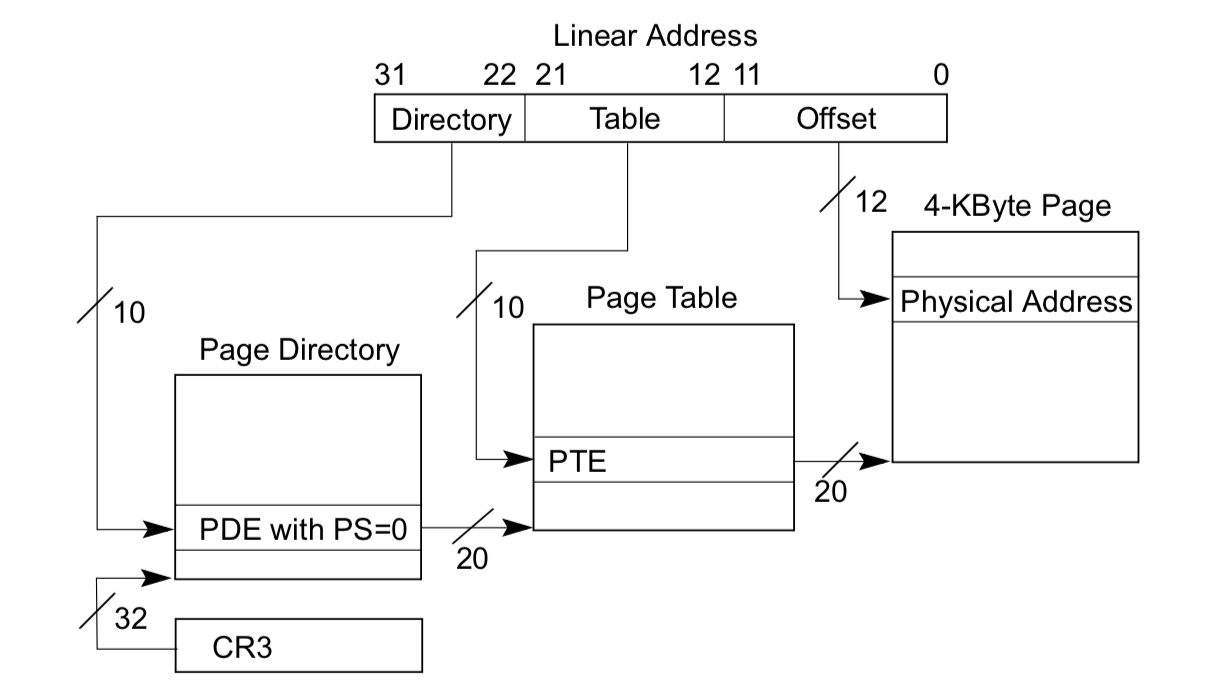
\includegraphics[width=10cm]{images/memory_page_table_32bits.png}
    \caption{\label{pic:memory_page_table_32bits} Table de pages utilisant 32 bits de l'adresse virtuelle dans une table à 3 niveaux \cite{intel64and}}.
\end{figure}

\begin{figure}
    \center
    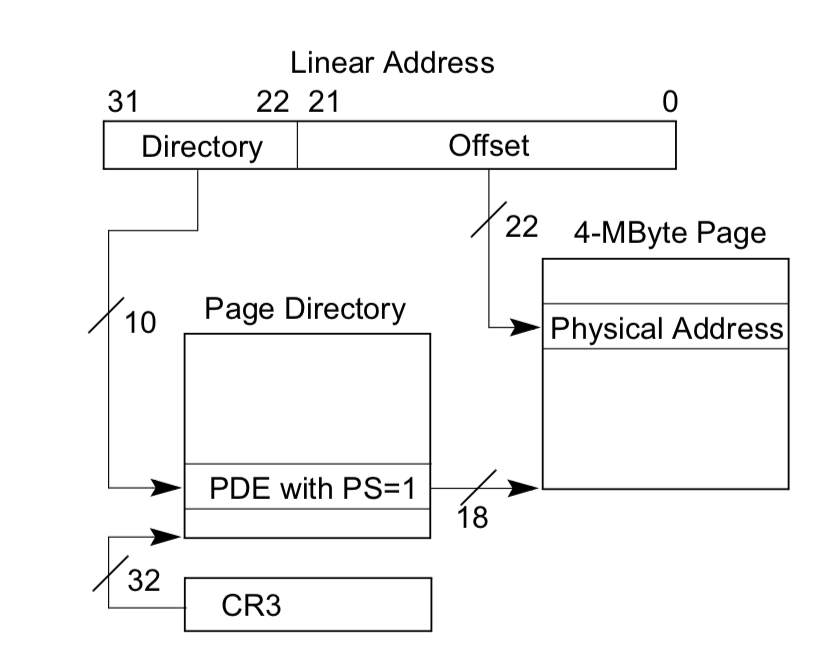
\includegraphics[width=10cm]{images/memory_page_table_32bits_large.png}
    \caption{\label{pic:memory_page_table_32bits_large} Table de pages pour des page large de 2 MiB\cite{intel64and}}.
\end{figure}


\begin{figure}
    \center
    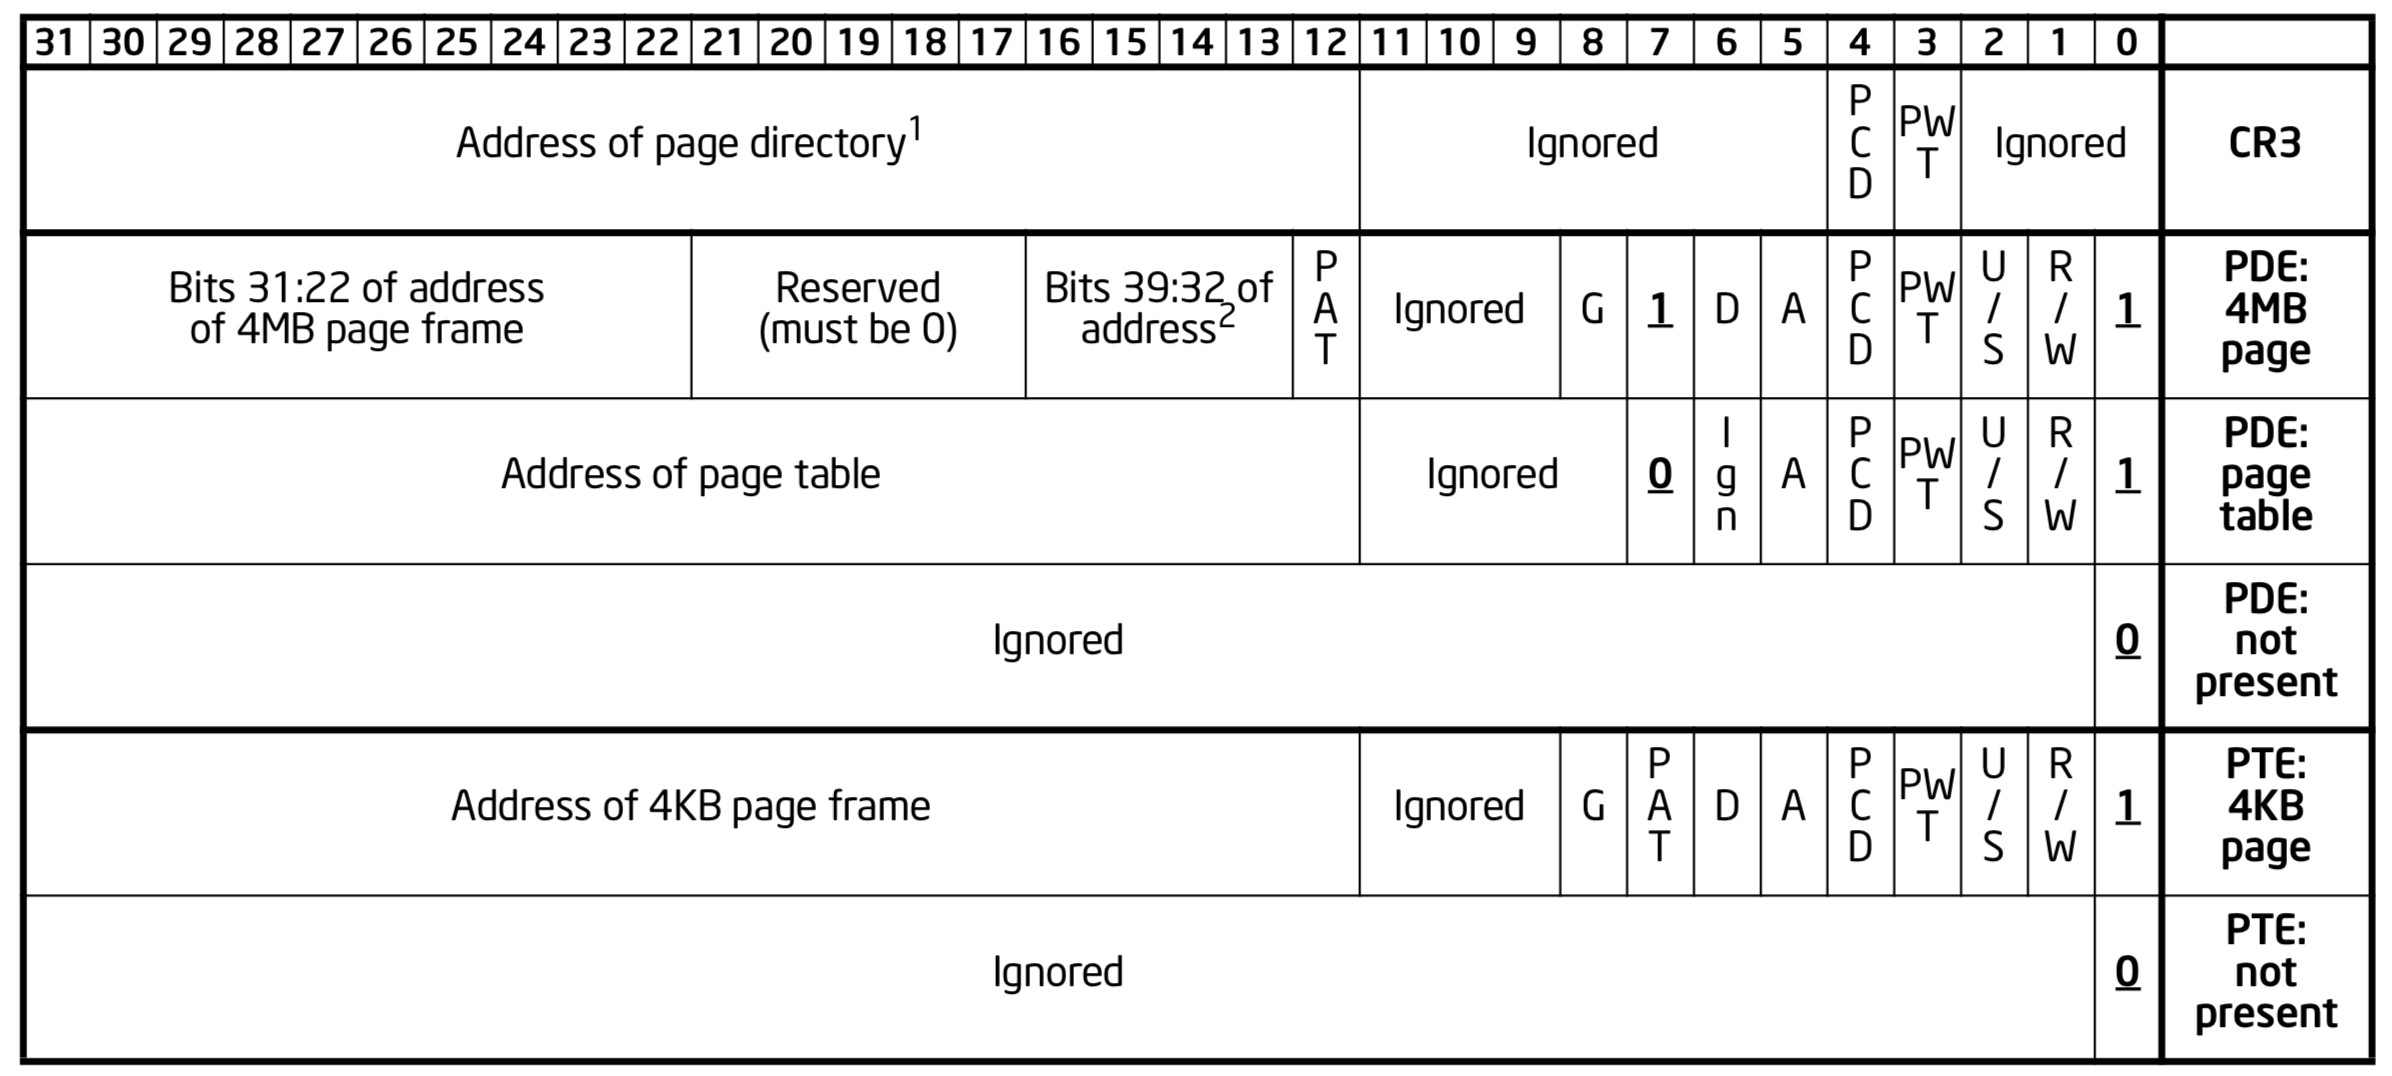
\includegraphics[width=10cm]{images/memory_page_table_entry_intel.png}
    \caption{\label{pic:memory_page_table_entry_intel} Structure d'une entrée dans la table de page \cite{intel64and}}.
\end{figure}



%\begin{figure}[p]
  %\centering
  %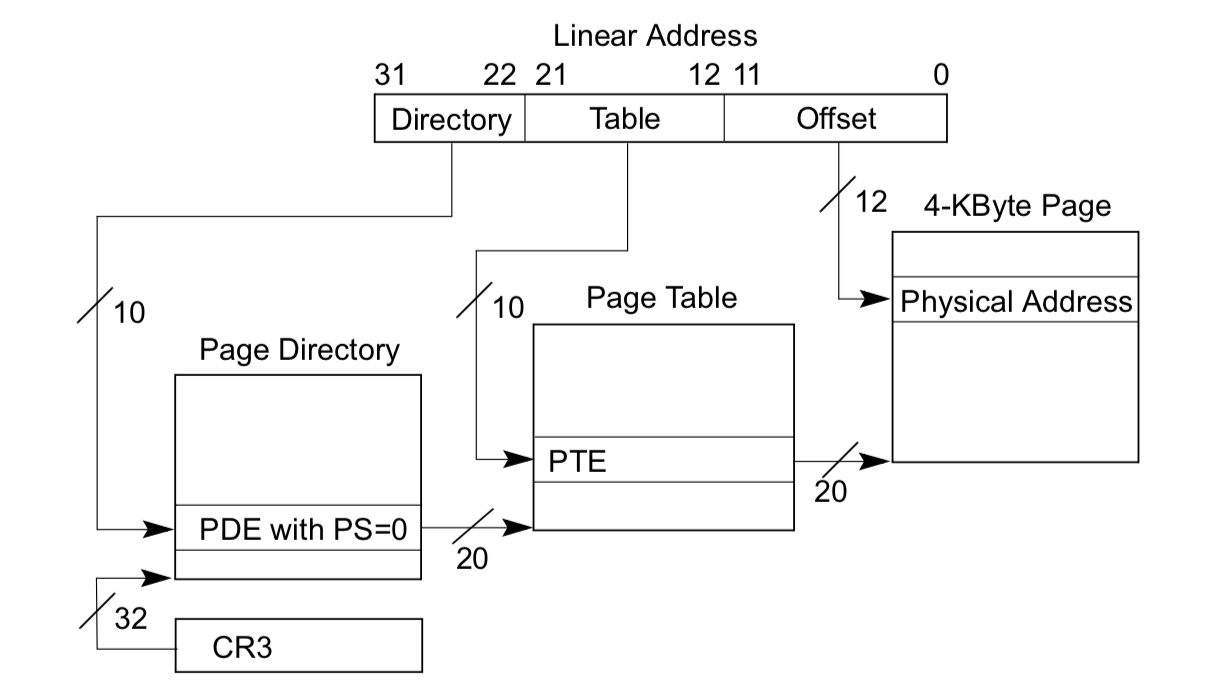
\includegraphics[width=0.2\textwidth]{images/memory_page_table_32bits.png}
  %\caption{Capt1.}
  %\label{fig:lab1}
  %\centering
  %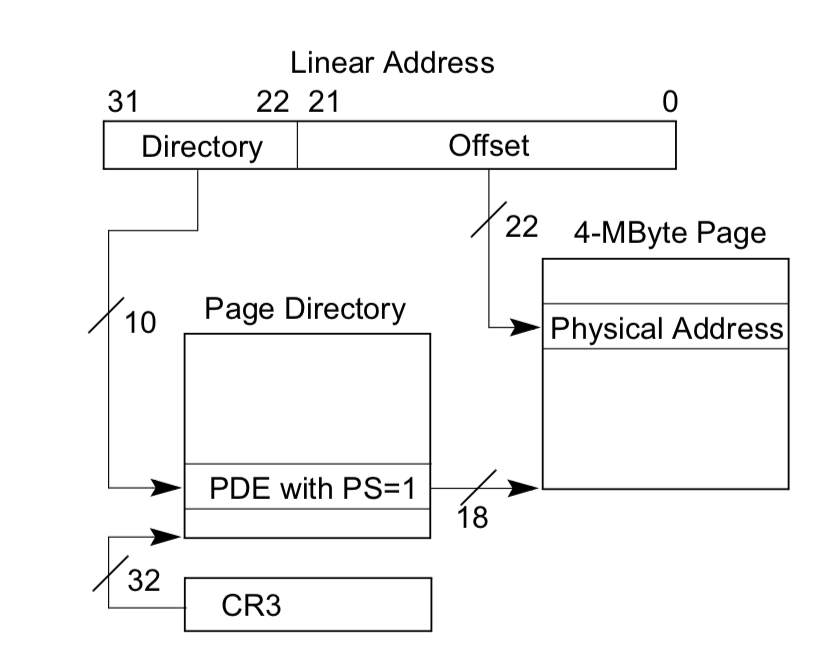
\includegraphics[width=0.2\textwidth]{images/memory_page_table_32bits_large.%png}
  %\caption{Capt2.}
  %\label{fig:lab2}
  %\centering
  %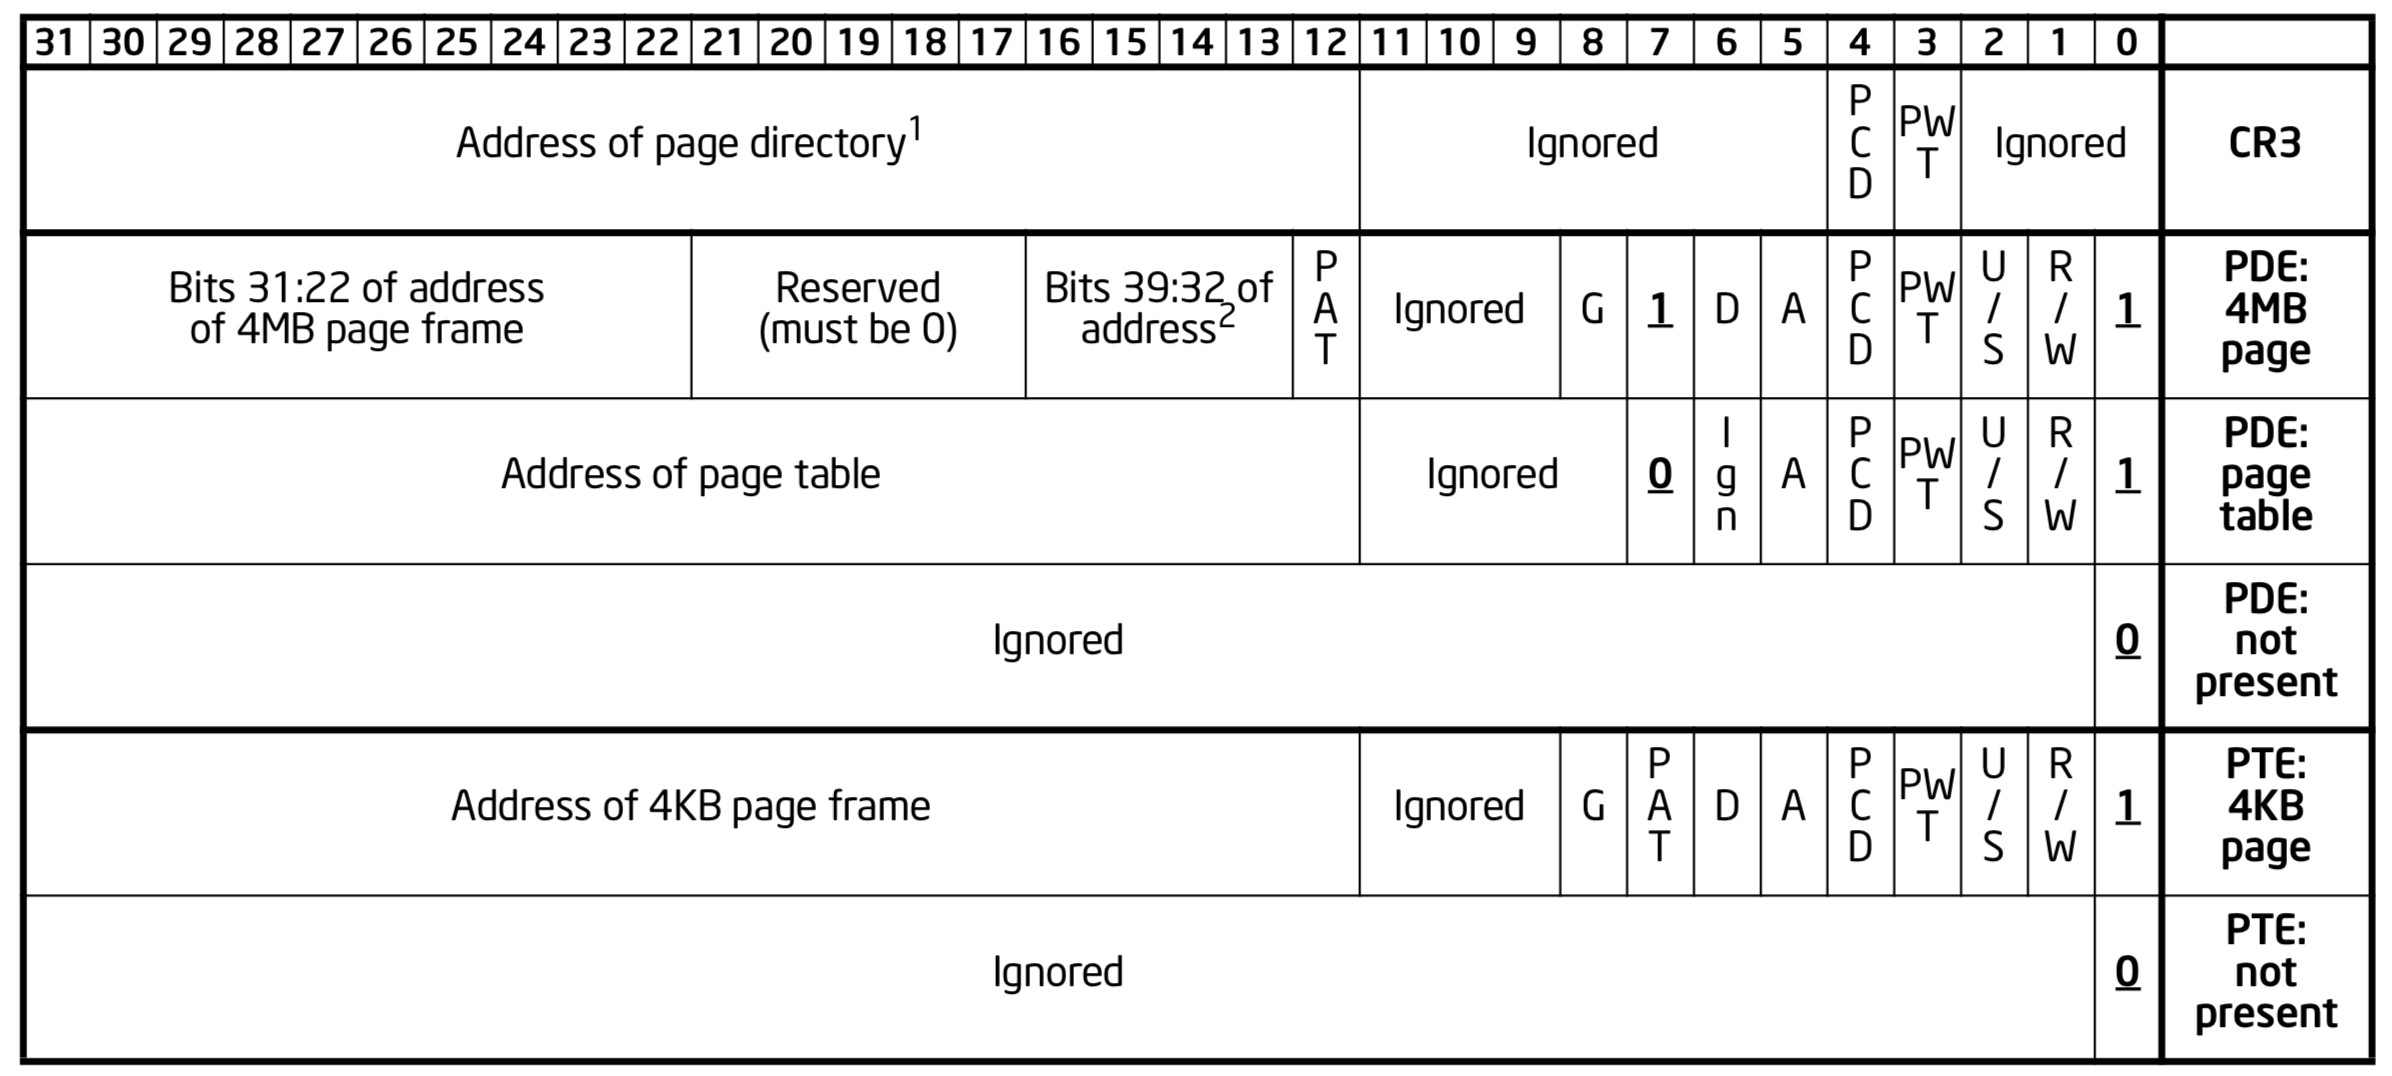
\includegraphics[width=0.2\textwidth]{images/memory_page_table_entry_intel.p%ng}
  %\caption{capt3.}
  %\label{fig:lab3}
%\end{figure}

\bibliographystyle{StyleThese}
\bibliography{These}

  \printindex


\cleardoublepage

\begin{vcenterpage}
\noindent\rule[2pt]{\textwidth}{0.5pt}
\begin{center}
{\large\textbf{Titre de la thèse\\}}
\end{center}
{\large\textbf{Abstract:}}
Résumé en anglais
\\
{\large\textbf{Keywords:}}
a,e,i,o,u,y
\\
\noindent\rule[2pt]{\textwidth}{0.5pt}
\end{vcenterpage}

\end{document}
